\documentclass{article}
\usepackage{mlnotes}

% grafici
\usepackage{pgfplots}
\usepackage{float}
\usepgfplotslibrary{statistics}
\pgfplotsset{compat=1.18}
% Definizione manuale della funzione di densità Gaussiana
\pgfmathdeclarefunction{gauss}{3}{%
  \pgfmathparse{1/(#3*sqrt(2*pi))*exp(-((#1-#2)^2)/(2*#3^2))}%
}

\renewcommand{\coursetitle}{Introduzione al Machine Learning}

\renewcommand{\notedate}{%
    Appunti del corso tenuto dal \textbf{Prof. Francesco Morandin} \\
    \medskip % Aggiunge un piccolo spazio verticale
    Università degli Studi di Parma \\
    Anno Accademico 2025/2026
}

\renewcommand{\coursecode}{000}

\begin{document}
\maketitle

\tableofcontents

\section*{Disclaimer}
\vfill
\begin{nota*}{}
I seguenti appunti sono stati generati a partire dal materiale
didattico e dalle note ufficiali del corso 'Introduzione al Machine Learning'.
Il contenuto è stato riorganizzato, formattato e parzialmente rielaborato con
l'ausilio di AI al fine di creare un documento coeso e ottimizzato per lo studio.

\medskip

Si raccomanda di fare sempre riferimento al materiale originale fornito dal
docente per garantire la massima accuratezza.
\end{nota*}
\vfill

\section{Ripasso Proprietà Variabili Aleatorie}\label{sec:ripasso_va}

\subsection{Definizioni Generali}\label{ssec:def_generali}
Ripassiamo i concetti fondamentali di Funzione di Ripartizione Cumulativa (CDF), Funzione di Densità di Probabilità (PDF) per variabili continue, e Funzione di Massa di Probabilità (PMF) per variabili discrete.

\begin{definizione}{Funzione di Ripartizione Cumulativa (CDF)}{cdf}
La CDF, indicata con \( F_X(t) \), descrive la probabilità che una variabile aleatoria (v.a.) \( X \) assuma un valore minore o uguale a \( t \).
\[
F_X(t) = P(X \le t)
\]
La CDF è una funzione non decrescente con valori compresi tra 0 e 1. Per una v.a. continua, la CDF è una funzione continua, mentre per una v.a. discreta è una funzione a gradini.
\end{definizione}

\begin{definizione}{PDF (per v.a. continue) e PMF (per v.a. discrete)}{pdf_pmf}
\begin{itemize}
    \item La \textbf{Funzione di Densità di Probabilità (PDF)}, \( f(t) \), per una v.a. continua, è la derivata della CDF. L'area sottesa alla curva della PDF tra due punti \( a \) e \( b \) rappresenta la probabilità che la variabile cada in quell'intervallo.
    \[
    f(t) = F'(t) \quad \text{e} \quad P(a < X \le b) = \int_a^b f(t) \,dt = F(b) - F(a)
    \]
    \item La \textbf{Funzione di Massa di Probabilità (PMF)}, \( \varphi_X(k) \), per una v.a. discreta, dà la probabilità esatta che la variabile assuma il valore \( k \).
    \[
    \varphi_X(k) = P(X = k) = F_X(k) - F_X(k-1)
    \]
    La CDF può essere ottenuta sommando i valori della PMF.
    \[
    F_X(k) = \sum_{j \le k} \varphi_X(j)
    \]
\end{itemize}
\end{definizione}

\begin{nota}{Calcolo di probabilità tramite CDF}{calcolo_prob}
Ecco un riassunto delle formule per calcolare la probabilità di un evento usando la CDF:
\begin{itemize}
    \item \textbf{Coda sinistra (v.a. continue e discrete):} Probabilità che \( X \) sia minore o uguale ad \( a \).
    \[ P(X \le a) = F_X(a) \]
    \item \textbf{Coda destra (v.a. continue):} Probabilità che \( X \) sia maggiore di \( b \).
    \[ P(X > b) = 1 - F_X(b) \]
    \item \textbf{Coda destra (v.a. discrete):} Probabilità che \( X \) sia maggiore o uguale a \( b \).
    \[ P(X \ge b) = 1 - F_X(b-1) \]
    \item \textbf{Intervallo (v.a. continue):} Probabilità che \( X \) sia compreso tra \( a \) e \( b \).
    \[ P(a < X \le b) = F_X(b) - F_X(a) \]
    \item \textbf{Intervallo (v.a. discrete, estremi esclusi):} Probabilità che \( X \) sia strettamente compreso tra \( a \) e \( b \).
    \[ P(a < X < b) = P(X \le b-1) - P(X \le a) = F_X(b-1) - F_X(a) \]
\end{itemize}
\end{nota}

\subsection{Inversione della Formula}\label{ssec:inversione}

Un uso molto comune della CDF è il calcolo del \textbf{quantile}, ovvero l'inversione della formula per trovare il valore \( x \) corrispondente a una data probabilità cumulata.

\begin{nota}{Quantile}{quantile}
Il \textbf{quantile} di livello \(p \in (0,1)\) di una variabile aleatoria \(X\) è il valore soglia \(q_p\) tale che:
\[
P(X \leq q_p) = p.
\]
In altre parole, il quantile è l’inversa della funzione di ripartizione cumulativa (CDF): 
\[
q_p = F_X^{-1}(p).
\]
Esempi importanti sono la \textit{mediana} (\(p=0.5\)), i \textit{quartili} (\(p=0.25,0.75\)) e in generale i \textit{percentili}. 
Essi permettono di descrivere in modo sintetico la distribuzione di una variabile e sono usati in statistica descrittiva, test d’ipotesi e intervalli di confidenza.
\end{nota}
\begin{esempio}{Trovare un quantile da una probabilità}{inversione_gamma}
Supponiamo di voler trovare il valore \( x \) per cui la probabilità che una variabile con distribuzione Gamma \( \gamma(\alpha, \beta) \) sia minore o uguale a \( x \) sia almeno del 5\%.
\begin{enumerate}
    \item \textbf{Impostare la disequazione:}
    \[
    P(\text{gamma}(\alpha, \beta) \le x) \ge 0.05
    \]
    \item \textbf{Esprimere tramite CDF:}
    \[
    F_{\text{gamma}}(x) \ge 0.05
    \]
    \item \textbf{Applicare la funzione inversa della CDF ($F_g^{-1}$):} Poiché la CDF e la sua inversa sono funzioni crescenti, il verso della disuguaglianza non cambia.
    \[
    F_g^{-1}(F_g(x)) \ge F_g^{-1}(0.05)
    \]
    \item \textbf{Risolvere per \(x\):}
    \[
    x \ge F_g^{-1}(0.05)
    \]
\end{enumerate}
La conclusione è che tutti i valori di \( x \) maggiori o uguali al quantile al 5\% della distribuzione Gamma soddisfano la richiesta. In software come Excel, questo valore si calcola con la funzione \texttt{GAMMA.INV(0.05, alpha, beta)}.
\end{esempio}

\subsection{Inversione con Due Incognite}\label{ssec:inversione_due_incognite}
Spesso si cerca un intervallo \( [a, b] \) tale per cui la probabilità che una variabile aleatoria cada al suo interno sia pari a un valore prefissato (es. 90\% o 95\%), tipicamente per costruire intervalli di confidenza.
\[
P(X \in [a, b]) = 1 - \alpha
\]
Ad esempio, se vogliamo \( P(a \le X \le b) = 90\% \), la probabilità totale nelle code (a sinistra di \(a\) e a destra di \(b\)) deve essere del 10\%. Poiché ci sono infinite coppie \( (a, b) \) che soddisfano questa condizione, si usano dei criteri per scegliere una soluzione unica.

\begin{nota}{Criteri per la scelta dell'intervallo}{criteri_intervallo}
I tre criteri più comuni sono:
\begin{itemize}
    \item \textbf{Intervallo Canonico (o delle code uguali):} La probabilità residua \( \alpha \) viene divisa equamente tra le due code. Se \( \alpha = 10\% \), si pone il 5\% sulla coda sinistra e il 5\% sulla destra.
    \[
    a = F_X^{-1}(0.05) \quad \text{e} \quad b = F_X^{-1}(0.95)
    \]
    \item \textbf{Intervallo Arbitrario:} La probabilità \( \alpha \) viene suddivisa in modo arbitrario, purché la somma sia corretta. Ad esempio, si potrebbe avere una coda sinistra con il 7\% di probabilità e una destra con il 3\%.
    \item \textbf{Intervallo di ampiezza minima:} Si cerca l'intervallo \( [a, b] \) che, a parità di probabilità interna, ha la larghezza \( (b-a) \) più piccola possibile. Per una distribuzione unimodale continua, questo si ottiene quando la funzione di densità ha la stessa altezza agli estremi.
    \[
    f(a) = f(b)
    \]
\end{itemize}
\end{nota}

\begin{nota}{Caso delle distribuzioni simmetriche}{intervallo_simmetrico}
Se la distribuzione di probabilità è simmetrica e unimodale (es. Normale, t di Student), l'intervallo \textbf{canonico} (a code uguali) coincide con l'intervallo di \textbf{ampiezza minima}.
\end{nota}

\subsection{Proprietà di Simmetria e Correzione per la Continuità}

\begin{nota}{Simmetria della CDF per distribuzioni simmetriche}{simmetria_cdf}
Per una distribuzione simmetrica attorno a zero, come la Normale standard \( \mathcal{N}(0,1) \), la CDF \( \Phi(x) \) ha le seguenti proprietà:
\[
\Phi(-x) = 1 - \Phi(x) \implies \Phi(x) + \Phi(-x) = 1
\]
Questa proprietà si estende anche alla sua funzione inversa (la funzione quantile):
\[
\Phi^{-1}(\alpha) = - \Phi^{-1}(1-\alpha)
\]
Ciò significa che il quantile di livello \( \alpha \) è l'opposto del quantile di livello \( 1-\alpha \).
\end{nota}

\begin{nota}{Correzione per la Continuità}{correzione_continuita}
Quando si approssima una v.a. discreta (che assume valori interi) con una v.a. continua, si introduce un errore. La \textbf{correzione per la continuità} serve a ridurre questo errore.
Per calcolare \( P(X \le k) \) dove \( X \) è una v.a. discreta, usando la CDF continua \( F \) come approssimazione, è più accurato calcolare \( F \) nel punto \( k+0.5 \).
\[
F_X(k) = P(X_{\text{discreta}} \le k) \approx F_{\text{continua}}(k + 0.5)
\]
Questo perché \( k+0.5 \) è il punto medio tra \(k\) e \(k+1\), fornendo una stima migliore del valore della funzione a gradini discreta.
\end{nota}

\subsection{Generazione di v.a. con Legge Data}\label{ssec:generazione_va}
Il metodo dell'\textbf{Inverse Transform Sampling} (Campionamento tramite Inversione della Trasformata) permette di generare numeri casuali da qualsiasi distribuzione di probabilità di cui sia nota la CDF. Si basa sulla trasformazione integrale di probabilità.

\begin{proposizione}{Metodo dell'Inverse Transform Sampling}{its}
Sia \( F \) la CDF di una distribuzione target. Per generare un campione \( X \) da questa distribuzione:
\begin{enumerate}
    \item Si genera un numero casuale \( U \) da una distribuzione Uniforme in \( [0, 1] \).
    \item Si calcola \( X = F^{-1}(U) \), dove \( F^{-1} \) è la funzione quantile (l'inversa della CDF).
\end{enumerate}
La variabile aleatoria \( X \) così generata avrà come distribuzione proprio quella descritta da \( F \).
\end{proposizione}

\begin{esempio}{Generazione da una distribuzione Esponenziale}{gen_exp}
Vogliamo generare un campione da una distribuzione Esponenziale di parametro \( \lambda \).
\begin{enumerate}
    \item \textbf{CDF:} \( F(t) = 1 - e^{-\lambda t} \) per \( t \ge 0 \).
    \item \textbf{Inversa della CDF:} Poniamo \( y = 1 - e^{-\lambda t} \) e risolviamo per \( t \).
    \[
    1-y = e^{-\lambda t} \implies \log(1-y) = -\lambda t \implies t = -\frac{1}{\lambda}\log(1-y)
    \]
    Quindi \( F^{-1}(y) = -\frac{1}{\lambda}\log(1-y) \).
    \item \textbf{Generazione:} Generiamo \( U \sim \text{Unif}(0,1) \) e calcoliamo:
    \[
    X = F^{-1}(U) = -\frac{1}{\lambda}\log(1-U)
    \]
\end{enumerate}
\end{esempio}

\begin{dimostrazione}{Giustificazione del metodo}{its}
Vogliamo dimostrare che la CDF di \( X = F^{-1}(U) \) è proprio \( F \). Sia \( F_X(t) \) la CDF di \( X \).
\[
F_X(t) = P(X \le t) = P(F^{-1}(U) \le t)
\]
Poiché \( F \) è una funzione crescente, possiamo applicarla a entrambi i lati della disuguaglianza senza cambiarne il verso:
\[
P(F^{-1}(U) \le t) = P(U \le F(t))
\]
Dato che \( U \sim \text{Unif}(0,1) \), per definizione la sua CDF è \( F_U(y) = P(U \le y) = y \). Sostituendo \( y = F(t) \), otteniamo:
\[
P(U \le F(t)) = F(t)
\]
Abbiamo quindi dimostrato che \( F_X(t) = F(t) \), confermando che la variabile \( X \) generata ha la distribuzione desiderata.
\end{dimostrazione}

\subsection{CDF Empirica e Diagramma Q-Q}\label{ssec:ecdf_qq}
Quando non si conosce la vera distribuzione di un set di dati, si possono usare strumenti empirici per stimarla e visualizzarla.

\begin{definizione}{Funzione di Ripartizione Cumulativa Empirica (ECDF)}{ecdf}
Dato un campione di \( n \) osservazioni \( x_1, \dots, x_n \), la \textbf{CDF Empirica} \( \hat{F}_n(t) \) è la proporzione di osservazioni nel campione che sono minori o uguali a \( t \).
\[
\hat{F}_n(t) = \frac{\#\{i: x_i \le t\}}{n}
\]
Graficamente, è una funzione a gradini che aumenta di \( 1/n \) in corrispondenza di ogni dato osservato. La ECDF è una stima della vera CDF (sconosciuta) della popolazione da cui il campione è stato estratto.
\end{definizione}

\paragraph{Diagramma Q-Q (Quantile-Quantile)}
Il diagramma Q-Q è uno degli strumenti grafici più efficaci per confrontare la distribuzione dei dati con una distribuzione teorica. L'idea è quella di plottare i quantili campionari (i dati ordinati) contro i quantili teorici della distribuzione di riferimento.

Se i dati seguono la distribuzione teorica, i punti sul grafico si allineano lungo una retta. Per verificare l'ipotesi di normalità (o gaussianità), si costruisce il grafico plottando i punti:
\[
\left( \Phi^{-1}\left( \frac{i-0.5}{n} \right), x_{(i)} \right)
\]
dove \( x_{(i)} \) è l'i-esimo dato ordinato e \( \Phi^{-1} \) è la funzione quantile della Normale standard.

\begin{nota}{Derivazione Matematica e Interpretazione}{qq_plot_logic}
La linearità del grafico Q-Q per dati Normali deriva da una relazione matematica precisa.

\paragraph{Relazione Fondamentale.}
Supponiamo che i nostri dati \( x_i \) seguano una distribuzione Normale \( \mathcal{N}(\mu, \sigma^2) \). Allora, ogni punto può essere espresso in termini di un quantile \( p_i \) e della funzione quantile inversa della Normale standard, \( \Phi^{-1} \).
\[
p_i = \Phi\left(\frac{x_i - \mu}{\sigma}\right) \iff x_i = \mu + \sigma \Phi^{-1}(p_i)
\]
Questa equazione mostra che ogni quantile dei nostri dati, \( x_i \), è una funzione lineare del quantile corrispondente di una Normale standard, \( \Phi^{-1}(p_i) \).

\paragraph{Costruzione del Grafico.}
Per costruire il grafico, confrontiamo i quantili campionari (i nostri dati ordinati) con i quantili teorici.
\begin{itemize}
    \item \textbf{Asse Y (Quantili Campionari):} Utilizziamo i dati osservati e ordinati: \[ x_{(1)}, x_{(2)}, \dots, x_{(n)} \]
    \item \textbf{Asse X (Quantili Teorici):} Dobbiamo calcolare i quantili teorici corrispondenti. Se i dati fossero Normali, le probabilità cumulate \( p_{(i)} \) associate a ogni \( x_{(i)} \) sarebbero uniformemente distribuite. Approssimiamo queste probabilità con le posizioni di plotting:
    \[
    p_{(i)} \approx \frac{i-0.5}{n}, \quad \text{per } i=1, \dots, n
    \]
    I quantili teorici della Normale standard sono quindi:
    \[
    z_i = \Phi^{-1}\left( \frac{i-0.5}{n} \right)
    \]
\end{itemize}

\paragraph{Interpretazione.}
Il diagramma Q-Q plotta i punti \( (z_i, x_{(i)}) \). Se l'ipotesi di normalità è vera, allora, sostituendo nell'equazione fondamentale, otteniamo:
\[
x_{(i)} \approx \mu + \sigma \Phi^{-1}(p_{(i)}) \approx \mu + \sigma z_i
\]
I punti del grafico \( (z_i, x_{(i)}) \) dovrebbero quindi giacere approssimativamente sulla retta \( y = \mu + \sigma z \). Una deviazione sistematica da questa retta indica che i dati non seguono una distribuzione Normale.
\end{nota}

\section{Leggi di Variabili Aleatorie Importanti}\label{sec:leggi_va}

\subsection{Distribuzione Gaussiana (o Normale)}
La distribuzione Gaussiana è una delle più importanti in statistica, descrivendo molti fenomeni naturali che risultano dalla somma di numerosi piccoli effetti indipendenti.

\begin{definizione}{Distribuzione Gaussiana}{gaussiana}
Una variabile aleatoria \(X\) segue una distribuzione Gaussiana con media \(\mu\) e varianza \(\sigma^2\), indicata con \(X \sim \mathcal{N}(\mu, \sigma^2)\), se la sua funzione di densità di probabilità (PDF) è:
\[
f(x) = \frac{1}{\sqrt{2\pi\sigma^2}} \exp\left\{ -\frac{(x-\mu)^2}{2\sigma^2} \right\}, \quad x \in \mathbb{R}
\]

\end{definizione}

\begin{nota}{Teorema del Limite Centrale (TLC)}{tlc}
Il TLC afferma che le grandezze casuali che sono la \textbf{somma} di tanti piccoli contributi indipendenti tendono ad avere una distribuzione Normale.
\end{nota}

\begin{proposizione}{Proprietà della Gaussiana}{gauss_props}
\begin{itemize}
    \item \textbf{Chiusura per trasformazioni lineari:} Se \(X \sim \mathcal{N}(\mu, \sigma^2)\), allora la trasformazione lineare \(a + bX\) segue ancora una distribuzione Normale:
    \[ a+bX \sim \mathcal{N}(a+b\mu, b^2\sigma^2) \]
    \item \textbf{Riproducibilità:} La somma di due v.a. Gaussiane \emph{indipendenti} è ancora una v.a. Gaussiana. Se \(X \sim \mathcal{N}(\mu_1, \sigma_1^2)\) e \(Y \sim \mathcal{N}(\mu_2, \sigma_2^2)\) sono indipendenti:
    \[ X+Y \sim \mathcal{N}(\mu_1+\mu_2, \sigma_1^2+\sigma_2^2) \]
    \item \textbf{CDF Canonica:} La CDF di una qualsiasi Normale può essere ricondotta a quella della Normale standard \( \Phi(t) = F_{\mathcal{N}(0,1)}(t) \):
    \[ F_{\mathcal{N}(\mu,\sigma^2)}(x) = P(X \le x) = \Phi\left(\frac{x-\mu}{\sigma}\right) \]
\end{itemize}
\end{proposizione}

\begin{figure}[H]
    \centering
    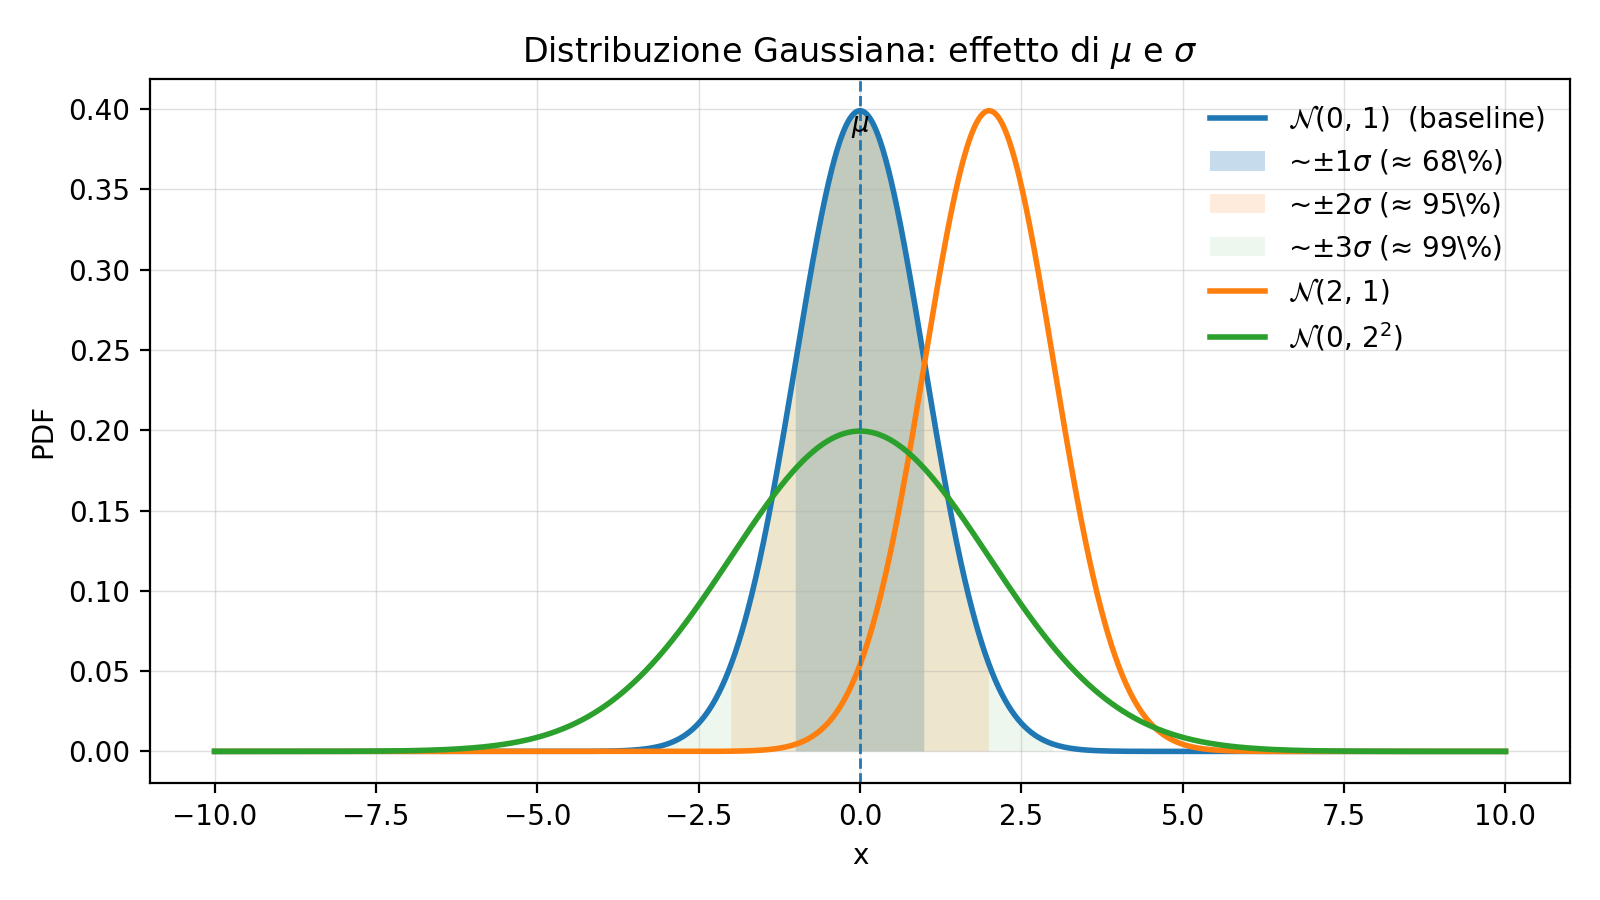
\includegraphics[width=0.8\textwidth]{images/th_01_03/gaussiana.png}
    \caption{Esempio di distribuzioni Gaussiane con \(\mu=0\) e \(\sigma\) variabile.}
    \label{fig:gaussiana}
\end{figure}

\subsection{Distribuzione Lognormale}
La Lognormale descrive grandezze che derivano dal \emph{prodotto} di molti fattori casuali.

\begin{definizione}{Distribuzione Lognormale}{lognormale}
Una variabile aleatoria \(X\) è Lognormale se il suo logaritmo naturale è una v.a. Normale. Se \(Y = \log X \sim \mathcal{N}(\mu, \sigma^2)\), allora si scrive \(X \sim \text{Lognorm}(\mu, \sigma^2)\). In altre parole, è l'esponenziale di una Gaussiana:
\[ X = e^Y, \quad \text{con } Y \sim \mathcal{N}(\mu, \sigma^2) \]
\end{definizione}

\begin{nota}{Origine della Lognormale}{lognorm_origin}
Una versione "moltiplicativa" del TLC afferma che le grandezze che sono il \textbf{prodotto} di tanti piccoli contributi indipendenti tendono ad avere una distribuzione Lognormale. Esempi tipici sono redditi, patrimoni e dimensioni di frammenti.
\end{nota}

\begin{proposizione}{Proprietà della Lognormale}{lognorm_props}
\begin{itemize}
    \item \textbf{Asimmetria:} È una distribuzione asimmetrica con una coda lunga a destra, adatta a modellare quantità che non possono essere negative ma possono assumere valori molto grandi.
    \item \textbf{Analisi dei dati:} Per analizzare dati lognormali, è pratica comune calcolarne il logaritmo e trattare i dati trasformati come Normali.
    \item \textbf{Media e Mediana:} A differenza della Normale, media e mediana non coincidono.
    \[ E(X) = e^{\mu + \frac{\sigma^2}{2}}, \quad \text{Mediana}(X) = e^\mu \]
\end{itemize}
\end{proposizione}

\begin{figure}[H]
    \centering
    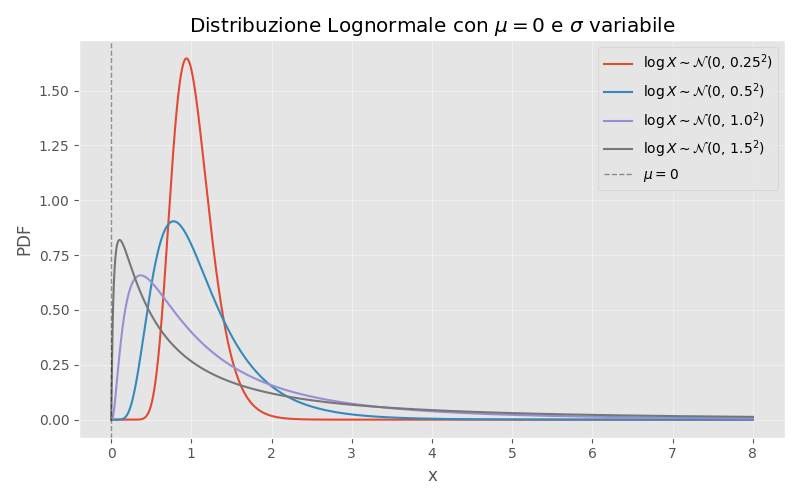
\includegraphics[width=0.8\textwidth]{images/th_01_03/lognormale.png}
    \caption{Esempio di distribuzioni Lognormali con \(\mu=0\) e \(\sigma\) variabile.}
    \label{fig:lognormale}
\end{figure}

\subsection{Distribuzione Esponenziale}
L'Esponenziale è la distribuzione di base per i tempi di attesa.

\begin{definizione}{Distribuzione Esponenziale}{esponenziale}
Una v.a. \(T\) segue una distribuzione Esponenziale di parametro \(\lambda > 0\), indicata con \(T \sim \text{Expo}(\lambda)\), se la sua PDF è:
\[
f_T(t) = \lambda e^{-\lambda t}, \quad t \ge 0
\]
Il parametro \(\lambda\) è chiamato \textbf{tasso} o \textbf{intensità}, e rappresenta il numero medio di eventi nell'unità di tempo.
\end{definizione}

\begin{proposizione}{Proprietà dell'Esponenziale}{expo_props}
\begin{itemize}
    \item \textbf{Versione continua della Geometrica:} Rappresenta il tempo di attesa per un evento che ha la stessa "probabilità" infinitesima di avvenire in ogni istante.
    \item \textbf{Assenza di memoria:} La probabilità di attendere ancora non dipende da quanto si è già atteso. Formalmente:
    \[ P(T > a+b \mid T > a) = P(T > b) \]
    \item \textbf{Applicazioni:} Modella tempi di attesa per eventi improvvisi e imprevedibili come guasti, telefonate, decadimenti radioattivi.
\end{itemize}
\end{proposizione}

\begin{figure}[H]
    \centering
    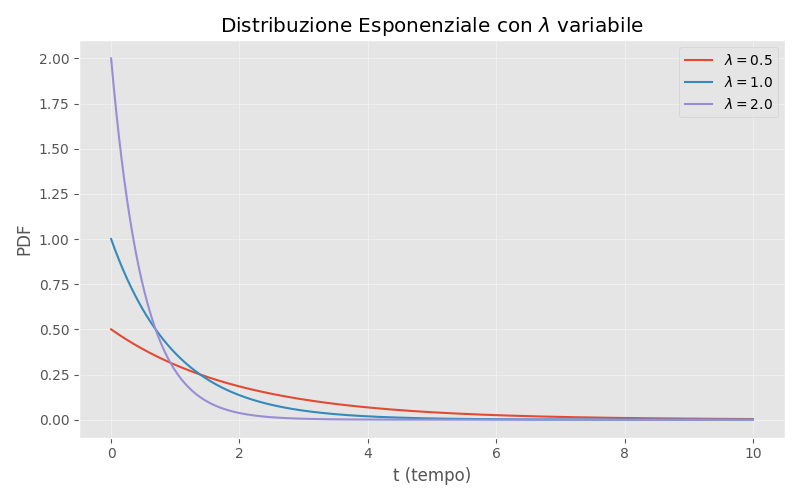
\includegraphics[width=0.8\textwidth]{images/th_01_03/esponenziale.png}
    \caption{Esempio di distribuzioni Esponenziali con \(\lambda\) variabile.}
    \label{fig:esponenziale}
\end{figure}

\subsection{Distribuzione Gamma}
La distribuzione Gamma è una generalizzazione dell'Esponenziale e della Chi-Quadro, molto flessibile per modellare tempi di attesa.

\begin{definizione}{Distribuzione Gamma}{gamma}
Una v.a. \(X\) segue una distribuzione Gamma definita da un parametro di forma \(\alpha>0\) e un parametro di tasso \(\lambda>0\). Si indica \(X \sim \text{Gamma}(\alpha, \lambda)\). La sua PDF è:
\[
f(t) = \frac{\lambda^\alpha}{\Gamma(\alpha)} t^{\alpha-1} e^{-\lambda t}, \quad t>0
\]
dove \(\Gamma(\alpha)\) è la funzione Gamma di Eulero. Una parametrizzazione alternativa usa un parametro di scala \(\beta = 1/\lambda\).
\end{definizione}

\begin{proposizione}{Proprietà della Gamma}{gamma_props}
\begin{itemize}
    \item \textbf{Riproducibilità:} La somma di v.a. Gamma indipendenti con lo stesso tasso \(\lambda\) è ancora una Gamma. Se \(X \sim \text{Gamma}(\alpha_1, \lambda)\) e \(Y \sim \text{Gamma}(\alpha_2, \lambda)\) sono indipendenti:
    \[ X+Y \sim \text{Gamma}(\alpha_1+\alpha_2, \lambda) \]
    \item \textbf{Scalatura:} Se \(X \sim \text{Gamma}(\alpha, \lambda)\), allora \(cX \sim \text{Gamma}(\alpha, \lambda/c)\).
    \item \textbf{Media e Varianza:}
    \[ E(X) = \frac{\alpha}{\lambda}, \quad \text{Var}(X) = \frac{\alpha}{\lambda^2} \]
\end{itemize}
\end{proposizione}

\begin{figure}[H]
    \centering
    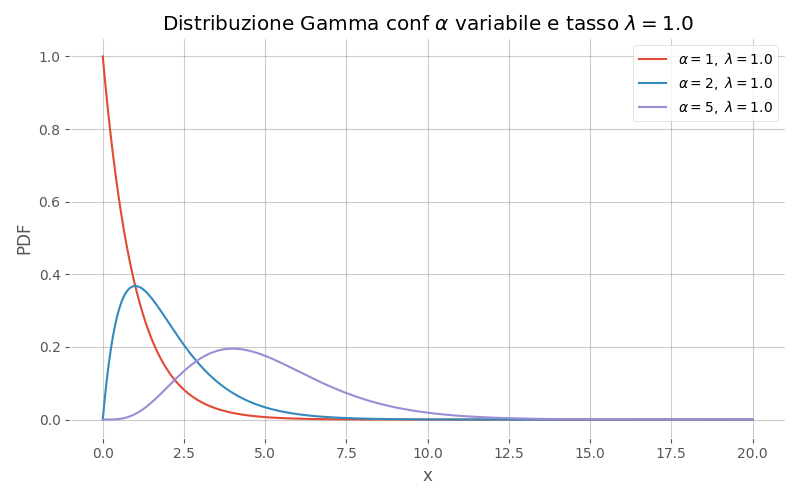
\includegraphics[width=0.8\textwidth]{images/th_01_03/gamma.png}
    \caption{Esempio di distribuzioni Gamma con \(\alpha\) variabili e \(\lambda\) costante.}
    \label{fig:gamma}
\end{figure}

\begin{nota}{Casi Particolari della Gamma}{gamma_casi}
\begin{itemize}
    \item \textbf{Esponenziale:} Per \(\alpha=1\), la Gamma diventa un'Esponenziale: \(\text{Gamma}(1, \lambda) \equiv \text{Expo}(\lambda)\).
    \item \textbf{Erlang:} Se \(\alpha=n\) è un intero, la distribuzione si chiama Erlang ed è la somma di \(n\) v.a. \(\text{Expo}(\lambda)\) indipendenti.
    \item \textbf{Chi-Quadro:} È un altro caso speciale, fondamentale in statistica.
\end{itemize}
\end{nota}

\subsection{Distribuzione Chi-Quadro}
\begin{definizione}{Distribuzione Chi-Quadro}{chi_quadro}
Una v.a. \(W\) segue una distribuzione Chi-Quadro con \(k\) gradi di libertà, \(W \sim \chi^2(k)\), se è la somma dei quadrati di \(k\) v.a. Normali standard indipendenti.
\[
W = \sum_{i=1}^k Z_i^2, \quad \text{dove } Z_i \sim \mathcal{N}(0,1) \text{ i.i.d.}
\]
È un caso particolare della Gamma: \( \chi^2(k) \equiv \text{Gamma}(k/2, 1/2) \).
\end{definizione}

\begin{nota}{Proprietà della Chi-Quadro}{chi_props}
Derivando dalla Gamma, si ottiene:
\[ E(W) = k, \quad \text{Var}(W) = 2k \]
Inoltre, poiché \( Z^2 \sim \chi^2(1) \), si ha che \(\chi^2(1) \equiv \text{Gamma}(1/2, 1/2)\).
\end{nota}

\begin{figure}[H]
    \centering
    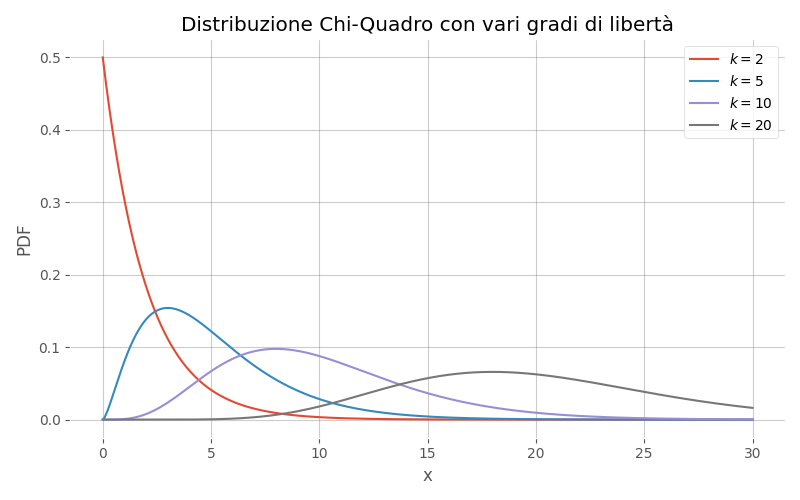
\includegraphics[width=0.8\textwidth]{images/th_01_03/chi2.png}
    \caption{Esempio di distribuzioni Chi-Quadro con \(k\) variabili.}
    \label{fig:chi2}
\end{figure}

\subsection{Il Processo di Poisson}
Il processo di Poisson descrive il verificarsi di eventi casuali nel tempo.

\begin{definizione}{Processo di Poisson}{poisson_proc}
Un processo di Poisson è una sequenza di eventi istantanei tali che i tempi di inter-arrivo tra un evento e il successivo sono variabili aleatorie indipendenti e identicamente distribuite (i.i.d.) come un'Esponenziale di tasso \(\lambda\).
\end{definizione}

\begin{proposizione}{Componenti del Processo di Poisson}{poisson_comp}
\begin{itemize}
    \item \textbf{Tempi di inter-arrivo \(T_i\):} Il tempo tra l'evento \(i-1\) e l'evento \(i\).
    \[ T_i \sim \text{Expo}(\lambda) \text{ i.i.d.} \]
    \item \textbf{Tempo di arrivo dell'n-esimo evento \(S_n\):} È la somma dei primi \(n\) tempi di inter-arrivo.
    \[ S_n = \sum_{i=1}^n T_i \sim \text{Gamma}(n, \lambda) \]
    \item \textbf{Numero di eventi in \([0, t]\), \(N_t\):} Il conteggio degli eventi fino a un certo istante \(t\). Segue una distribuzione di Poisson.
    \[ N_t \sim \text{Pois}(\lambda t) \]
\end{itemize}
\end{proposizione}

\subsection{Distribuzione Binomiale}

\begin{definizione}{Distribuzione Binomiale}{binomiale}
Una variabile aleatoria discreta \(X\) segue una distribuzione Binomiale con parametri \(n\) (un intero positivo) e \(p \in [0,1]\), indicata con \(X \sim \text{Bin}(n,p)\), se la sua funzione di massa di probabilità (PMF) è:
\[
P(X=k) = \binom{n}{k} p^k (1-p)^{n-k}, \quad k=0, 1, \dots, n \text{}
\]
\end{definizione}

\begin{proposizione}{Proprietà della Binomiale}{binom_props}
\begin{itemize}
    \item Il caso con \(n=1\) è detto distribuzione \textbf{Bernoulliana}.
    \item La Binomiale rappresenta il numero di successi in \(n\) prove indipendenti, ognuna con la stessa probabilità di successo \(p\). È la somma di \(n\) v.a. di Bernoulli i.i.d..
    \item \textbf{Riproducibilità:} La somma di v.a. Binomiali indipendenti con lo stesso parametro \(p\) è ancora una v.a. Binomiale. Se \(X_i \sim \text{Bin}(n_i, p)\) sono indipendenti:
    \[ \sum_{i=1}^{m} X_i \sim \text{Bin}\left(\sum_{i=1}^{m} n_i, p\right) \text{} \]
    \item \textbf{Media e Varianza:}
    \[ E(X) = np, \quad \text{Var}(X) = np(1-p) \]
\end{itemize}
\end{proposizione}

\begin{figure}[H]
    \centering
    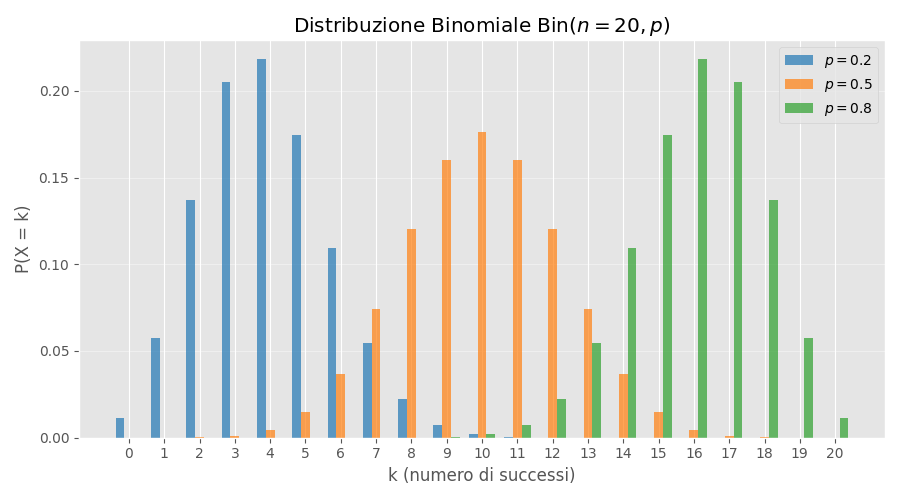
\includegraphics[width=0.8\textwidth]{images/th_01_03/binomiale.png}
    \caption{Esempio di distribuzioni Binomiali con \(n = 20\) e \(p\) variabile.}
    \label{fig:binomiale}
\end{figure}

\subsection{Distribuzione di Poisson}

\begin{definizione}{Distribuzione di Poisson}{poisson}
Una v.a. discreta \(X\) segue una distribuzione di Poisson di parametro \(\nu > 0\), indicata con \(X \sim \text{Pois}(\nu)\), se la sua PMF è:
\[
P(X=k) = \frac{\nu^k e^{-\nu}}{k!}, \quad k=0, 1, 2, \dots \text{}
\]
\end{definizione}

\begin{figure}[H]
    \centering
    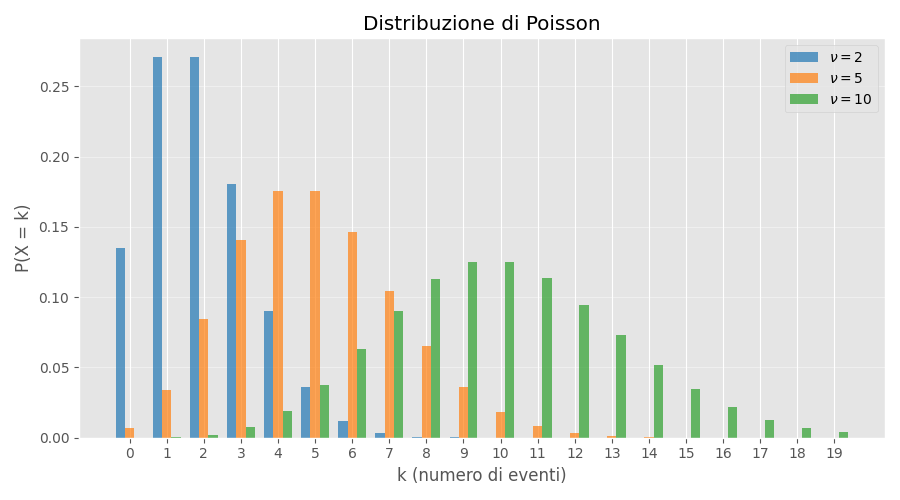
\includegraphics[width=0.8\textwidth]{images/th_01_03/poisson.png}
    \caption{Esempio di distribuzioni di Poisson con \(\nu\) variabile.}
    \label{fig:poisson}
\end{figure}

\begin{nota}{Relazione con la Binomiale}{pois_binom}
La distribuzione di Poisson è il limite della Binomiale per \(n\) grande e \(p\) piccolo. In pratica, se \(p \ll 1\), allora \(\text{Bin}(n,p) \approx \text{Pois}(np)\). Per questo motivo, è usata per contare il numero di successi (eventi rari) in scenari con un gran numero di prove, come il numero di gol in una partita o il numero di iscritti a un corso.

\begin{figure}[H]
    \centering
    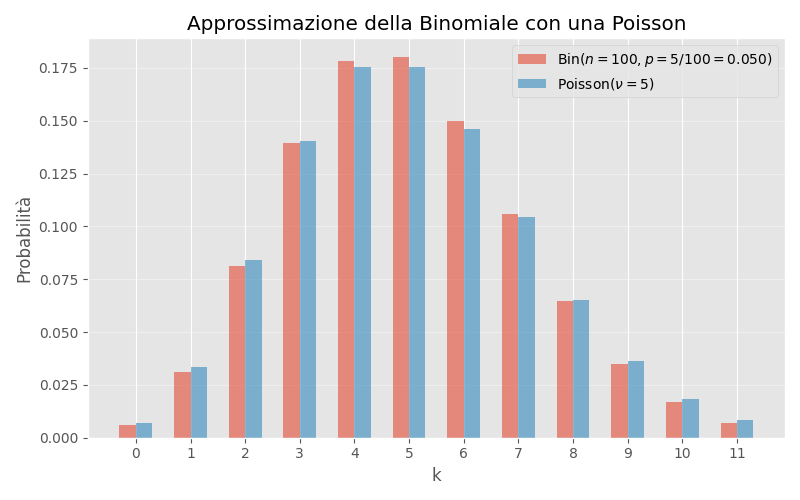
\includegraphics[width=0.8\textwidth]{images/th_01_03/binomiale_vs_poisson.png}
    \caption{Esempio di approssimazione della Binomiale con la Poisson.}
    \label{fig:binomiale_vs_poisson}
\end{figure}

\end{nota}

\begin{proposizione}{Proprietà della Poisson}{pois_props}
\begin{itemize}
    \item \textbf{Riproducibilità:} La somma di v.a. di Poisson indipendenti è ancora una v.a. di Poisson. Se \(X_i \sim \text{Pois}(\nu_i)\) sono indipendenti:
    \[ \sum_{i=1}^{m} X_i \sim \text{Pois}\left(\sum_{i=1}^{m} \nu_i\right) \text{} \]
    \item \textbf{Media e Varianza:} A differenza della Binomiale, media e varianza coincidono.
    \[ E(X) = \nu, \quad \text{Var}(X) = \nu \text{} \]
\end{itemize}
\end{proposizione}

\subsection{Distribuzione Uniforme}

\begin{definizione}{Distribuzione Uniforme Continua}{uniforme}
Una v.a. \(X\) segue una distribuzione Uniforme sull'intervallo \([a,b]\), con \(a<b\) reali, se la sua PDF è costante su quell'intervallo e zero altrove.
\[
f_X(t) = \frac{1}{b-a}, \quad \text{per } a < t < b \text{}
\]
La funzione \texttt{rand()} nei linguaggi di programmazione genera tipicamente campioni da \(\text{Unif}(0,1)\).
\end{definizione}

\begin{proposizione}{Proprietà dell'Uniforme}{unif_props}
\begin{itemize}
    \item \textbf{Media e Varianza:}
    \[ E(X) = \frac{a+b}{2}, \quad \text{Var}(X) = \frac{(b-a)^2}{12} \]
    \item È una classe chiusa per trasformazioni lineari.
\end{itemize}
\end{proposizione}

\begin{figure}[H]
    \centering
    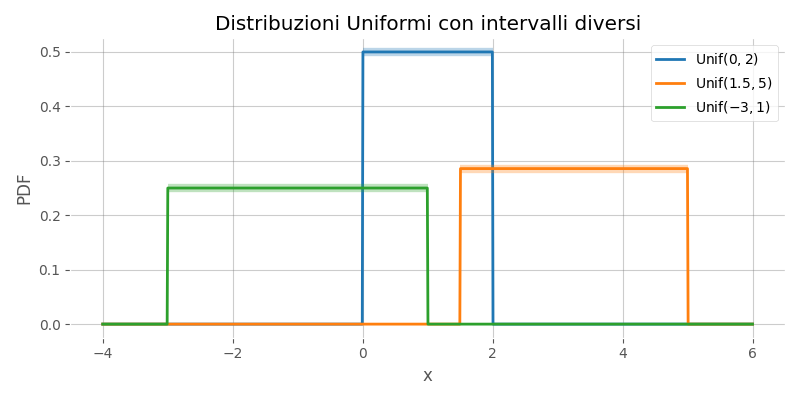
\includegraphics[width=0.8\textwidth]{images/th_01_03/uniforme.png}
    \caption{Esempio di distribuzioni Uniformi con \(a\) e \(b\) variabili.}
    \label{fig:uniforme}
\end{figure}

\subsection{Distribuzione Beta}

\begin{definizione}{Distribuzione Beta}{beta}
Una v.a. \(X\) segue una distribuzione Beta con parametri di forma \(\alpha, \beta > 0\), se la sua PDF è:
\[
f_X(t) = c_p t^{\alpha-1}(1-t)^{\beta-1}, \quad \text{per } 0 < t < 1 \text{}
\]
È una distribuzione molto flessibile, definita su un intervallo limitato.
\end{definizione}

\begin{figure}[H]
    \centering
    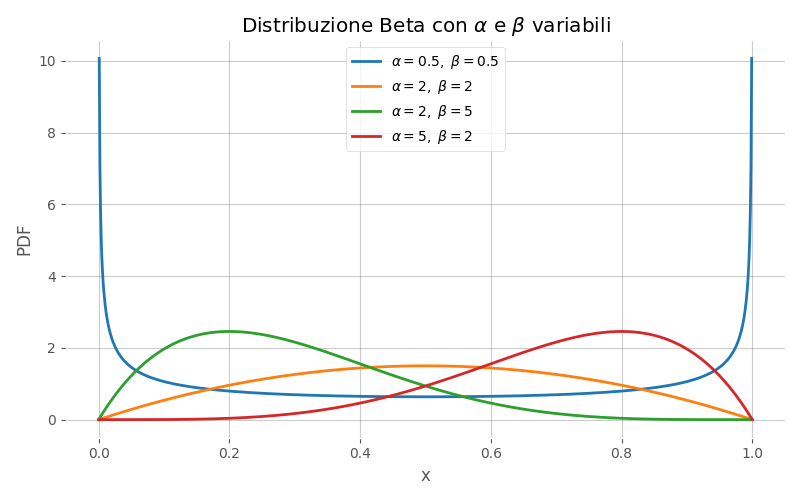
\includegraphics[width=0.8\textwidth]{images/th_01_03/beta.png}
    \caption{Esempio di distribuzioni Beta con \(\alpha\) e \(\beta\) variabili.}
    \label{fig:beta}
\end{figure}

\begin{nota}{Interpretazione della Beta}{beta_interp}
\begin{itemize}
    \item Il caso speciale \(\text{Beta}(1,1)\) corrisponde alla distribuzione \(\text{Unif}(0,1)\).
    \item \textbf{Statistica d'ordine:} La distribuzione \(\text{Beta}(m,n)\) è la distribuzione della \(m\)-esima variabile più piccola tra \(m+n-1\) v.a. \(\text{Unif}(0,1)\) indipendenti.
\end{itemize}
\end{nota}

\subsection{Distribuzione t di Student}

\begin{definizione}{Distribuzione t di Student}{t_student}
La distribuzione t di Student con \(k\) gradi di libertà, \(t(k)\), è definita operativamente dal rapporto tra una v.a. Normale standard e la radice di una Chi-Quadro indipendente, divisa per i suoi gradi di libertà.
Se \(Z \sim \mathcal{N}(0,1)\) e \(W \sim \chi^2(k)\) sono indipendenti, allora:
\[
T = \frac{Z}{\sqrt{W/k}} \sim t(k) \text{}
\]
\end{definizione}

\begin{proposizione}{Proprietà della t di Student}{t_props}
\begin{itemize}
    \item Ha una forma a campana simile alla Normale, ma con code più "pesanti".
    \item Per \(k \to \infty\), la distribuzione \(t(k)\) converge alla Normale standard \(\mathcal{N}(0,1)\).
    \item La media è \(E(T)=0\) (per \(k>1\)).
\end{itemize}
\end{proposizione}

\begin{figure}[H]
    \centering
    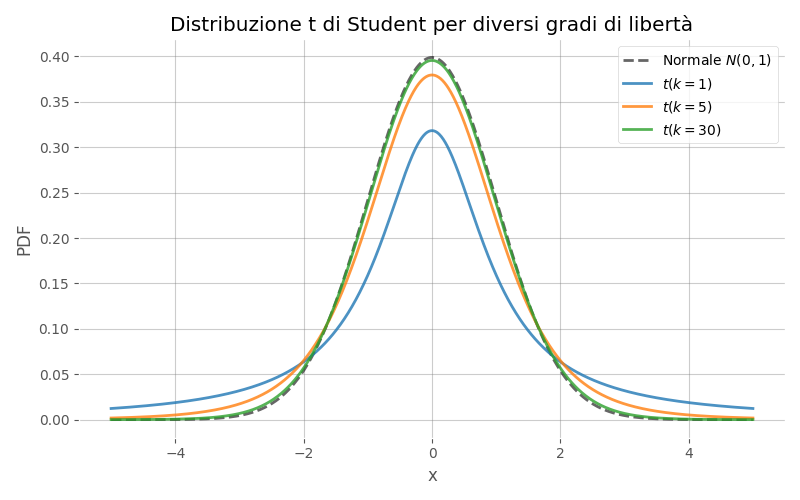
\includegraphics[width=0.8\textwidth]{images/th_01_03/t_student.png}
    \caption{Esempio di distribuzioni t di Student con \(k\) variabile.}
    \label{fig:t_student}
\end{figure}

\subsection{Distribuzione F di Fisher}

\begin{definizione}{Distribuzione F di Fisher}{f_fisher}
La distribuzione F di Fisher con \((m, n)\) gradi di libertà, \(F(m,n)\), è definita operativamente come il rapporto tra due v.a. Chi-Quadro indipendenti, ciascuna divisa per i propri gradi di libertà.
Se \(W_1 \sim \chi^2(m)\) e \(W_2 \sim \chi^2(n)\) sono indipendenti, allora:
\[
F = \frac{W_1/m}{W_2/n} \sim F(m,n) \text{}
\]
\end{definizione}

\begin{figure}[H]
    \centering
    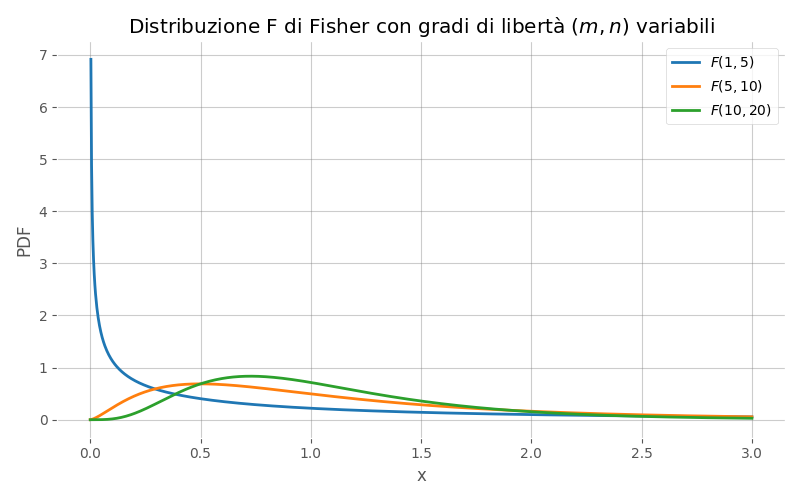
\includegraphics[width=0.8\textwidth]{images/th_01_03/f_fisher.png}
    \caption{Esempio di distribuzioni F di Fisher con \((m,n)\) variabili.}
    \label{fig:f_fisher}
\end{figure}

\begin{nota}{Uso della Distribuzione F}{f_uso}
È usata principalmente per confrontare due varianze campionarie. I parametri \(m\) e \(n\) sono i gradi di libertà del numeratore e del denominatore, rispettivamente.
\end{nota}

\subsection{Distribuzione Uniforme Discreta}

\begin{definizione}{Distribuzione Uniforme Discreta}{unif_discreta}
Una v.a. \(X\) segue una distribuzione Uniforme Discreta se può assumere \(n\) valori, \(\{1, 2, \dots, n\}\), ciascuno con la stessa probabilità. L'esempio classico è il lancio di un dado a \(n\) facce.
\[
P(X = i) = \frac{1}{n}, \quad \text{per } i=1, 2, \dots, n
\]
\end{definizione}

\begin{figure}[H]
    \centering
    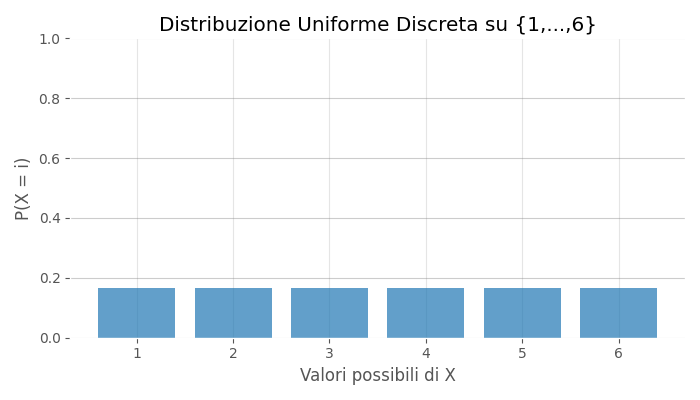
\includegraphics[width=0.8\textwidth]{images/th_01_03/uniforme_discreta.png}
    \caption{Esempio di distribuzioni Uniformi Discrete su \(\{1, 2, \dots, 6\}\).}
    \label{fig:uniforme_discreta}
\end{figure}

\begin{proposizione}{Proprietà dell'Uniforme Discreta}{unif_discreta_props}
\begin{itemize}
    \item \textbf{Non è riproducibile:} La somma di due o più v.a. uniformi discrete indipendenti non è più uniforme. La sua distribuzione tende a una forma a campana (analogo discreto del TLC).
    \item \textbf{Media e Varianza:}
    \[ E(X) = \frac{n+1}{2}, \quad \text{Var}(X) = \frac{n^2-1}{12} \]
\end{itemize}
\end{proposizione}

\subsection{Processo di Bernoulli e Distribuzioni Associate}
Molte distribuzioni discrete di base emergono dal \textbf{Processo di Bernoulli}, l'analogo a tempo discreto del Processo di Poisson.

\begin{definizione}{Processo di Bernoulli}{proc_bernoulli}
Un processo di Bernoulli è una sequenza di prove o esperimenti indipendenti, ciascuno con due soli esiti possibili: "successo" (con probabilità \(p\)) o "insuccesso" (con probabilità \(1-p\)).
\end{definizione}

\begin{nota}{Variabili aleatorie in un Processo di Bernoulli}{vars_bernoulli}
All'interno di un processo di Bernoulli si possono definire diverse variabili aleatorie di interesse:
\begin{itemize}
    \item \textbf{Numero di successi \(N_n\):} Il conteggio dei successi in \(n\) prove. Segue una distribuzione \(\text{Bin}(n,p)\).
    \item \textbf{Tempo del primo successo \(T_1\):} Il numero di prove necessarie per ottenere il primo successo. Segue una distribuzione \(\text{Geom}(p)\).
    \item \textbf{Tempo dell'm-esimo successo \(S_m\):} Il numero di prove necessarie per ottenere l'\(m\)-esimo successo. Segue una distribuzione \(\text{NegBin}(m,p)\).
\end{itemize}
\end{nota}

\subsection{Distribuzione Geometrica}

\begin{definizione}{Distribuzione Geometrica}{geometrica}
Una v.a. \(X\) segue una distribuzione Geometrica di parametro \(p \in (0,1]\) se la sua PMF è:
\[
P(X=k) = p(1-p)^{k-1}, \quad k=1, 2, 3, \dots
\]
Rappresenta il numero di prove necessarie per ottenere il primo successo in un processo di Bernoulli.
\end{definizione}

\begin{figure}[H]
    \centering
    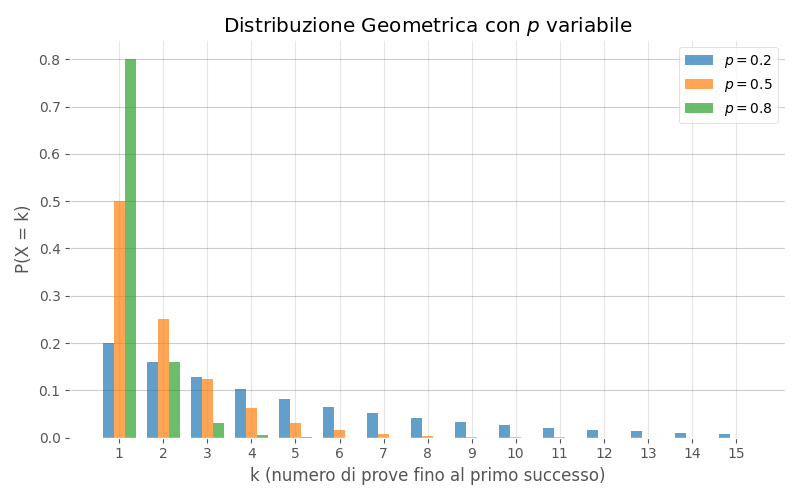
\includegraphics[width=0.8\textwidth]{images/th_01_03/geometrica.png}
    \caption{Esempio di distribuzioni Geometriche con \(p\) variabile.}
    \label{fig:geometrica}
\end{figure}

\begin{proposizione}{Proprietà della Geometrica}{geom_props}
\begin{itemize}
    \item È la versione discreta della distribuzione Esponenziale.
    \item \textbf{Media e Varianza:}
    \[ E(X) = \frac{1}{p}, \quad \text{Var}(X) = \frac{1-p}{p^2} \]
\end{itemize}
\end{proposizione}

\subsection{Distribuzione Binomiale Negativa}
Questa distribuzione generalizza la Geometrica al caso di \(r\) successi.

\begin{definizione}{Distribuzione Binomiale Negativa}{negbin}
Esistono due definizioni comuni per la Binomiale Negativa \(\text{NegBin}(r,p)\):
\begin{enumerate}
    \item \textbf{Numero di prove:} \(X\) è il numero totale di prove per ottenere \(r\) successi. La sua PMF è:
    \[ P(X=k) = \binom{k-1}{r-1}p^r(1-p)^{k-r}, \quad k=r, r+1, \dots \]
    \item \textbf{Numero di insuccessi:} \(\tilde{X}\) è il numero di insuccessi che avvengono prima di ottenere \(r\) successi. La sua PMF, usata spesso in software come SciPy, è:
    \[ P(\tilde{X}=k) = \binom{k+r-1}{k}p^r(1-p)^{k}, \quad k=0, 1, 2, \dots \]
\end{enumerate}
\end{definizione}

\begin{figure}[H]
    \centering
    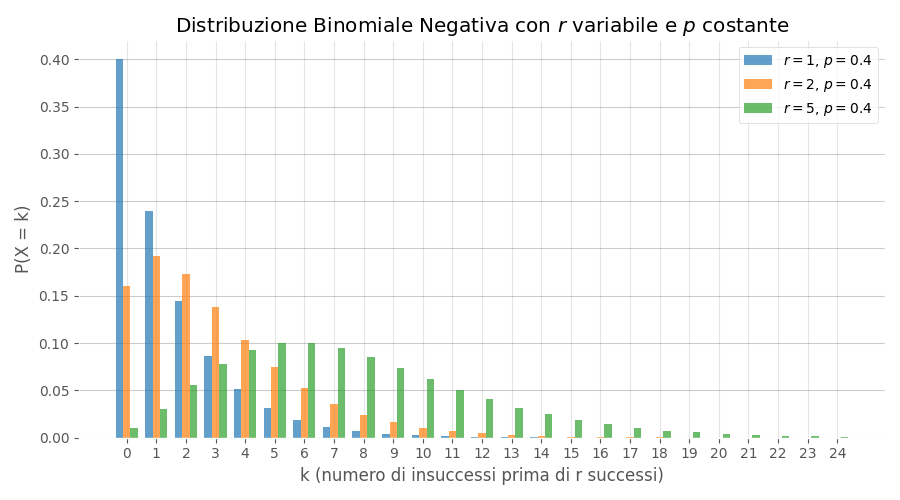
\includegraphics[width=0.8\textwidth]{images/th_01_03/negbin.png}
    \caption{Esempio di distribuzioni Binomiali Negative con \(r\) variabile e \(p\) costante per numero di insuccessi.}
    \label{fig:negbin}
\end{figure}


\begin{figure}[H]
    \centering
    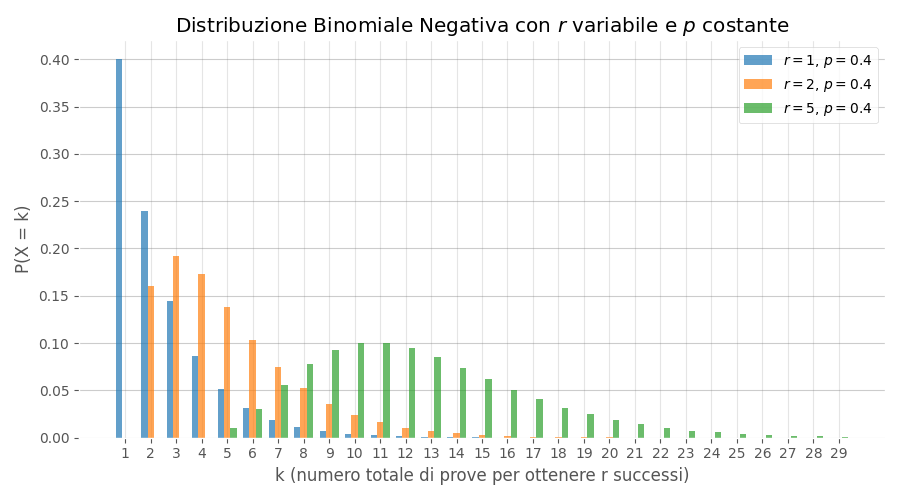
\includegraphics[width=0.8\textwidth]{images/th_01_03/negbin_trials.png}
    \caption{Esempio di distribuzioni Binomiali Negative con \(r\) variabile e \(p\) costante per numero di prove.}
    \label{fig:negbin_trials}
\end{figure}

\begin{proposizione}{Proprietà della Binomiale Negativa}{negbin_props}
\begin{itemize}
    \item Se \(r=1\), si ottiene la distribuzione Geometrica.
    \item \textbf{Riproducibilità:} La somma di v.a. Binomiali Negative indipendenti con lo stesso \(p\) è ancora una Binomiale Negativa. Se \(X_i \sim \text{NegBin}(r_i, p)\) sono indipendenti:
    \[ \sum X_i \sim \text{NegBin}\left(\sum r_i, p\right) \]
    \item \textbf{Media e Varianza (per la def. 1):}
    \[ E(X) = \frac{r}{p}, \quad \text{Var}(X) = \frac{r(1-p)}{p^2} \]
\end{itemize}
\end{proposizione}

\include{lectures/th_06}
\section{Vettori Aleatori e Machine Learning}\label{sec:va_ml}

\subsection{Apprendimento Supervisionato (Supervised Learning)}

\begin{definizione}{Apprendimento Supervisionato}{def:supervised_learning}
Nell'apprendimento supervisionato, l'obiettivo è predire una o più variabili di output a partire da un insieme di variabili di input (dette predittori).
\end{definizione}

\begin{esempio}{Casi d'uso}{supervised_cases}
Alcune applicazioni pratiche includono:
\begin{itemize}
    \item Prevedere le risorse necessarie (tempo, soldi, energia) per una commessa o un progetto.
    \item Prevedere il peso corporeo di un soggetto basandosi su altre misure fisiche.
    \item Classificare il contenuto di un'immagine, assegnandola a una categoria specifica.
\end{itemize}
\end{esempio}

\begin{figure}[ht]
\centering
\begin{tikzpicture}
\begin{axis}[
    width=12cm,
    height=6cm,
    xlabel={Statura ($y$)},
    ylabel={Densità},
    xtick={168, 175},
    ytick=\empty,
    axis y line=left,
    axis x line=bottom,
    enlarge x limits=0.1,
    samples=100,
    domain=140:210,
]

% Parametri delle distribuzioni
\def\muM{175} % Media maschi
\def\muF{168} % Media femmine
\def\sigmaVal{7} % Deviazione standard

% Distribuzione condizionata per X=0 (maschi)
\addplot[blue, thick] {gauss(x, \muM, \sigmaVal)};
\node[above, blue] at (axis cs:178, {gauss(175, \muM, \sigmaVal)}) {\(f_{Y|X}(y|X=0)\)};

% Distribuzione condizionata per X=1 (femmine)
\addplot[violet, thick] {gauss(x, \muF, \sigmaVal)};
\node[above, violet] at (axis cs:165, {gauss(168, \muF, \sigmaVal)}) {\(f_{Y|X}(y|X=1)\)};

% Distribuzione marginale di Y (curva verde)
\addplot[green!60!black, thick, dashed] {0.5*gauss(x, \muM, \sigmaVal) + 0.5*gauss(x, \muF, \sigmaVal)};

% Linee tratteggiate per indicare le medie
\draw[dashed] (axis cs:\muM, 0) -- (axis cs:\muM, {gauss(\muM, \muM, \sigmaVal)});
\draw[dashed] (axis cs:\muF, 0) -- (axis cs:\muF, {gauss(\muF, \muF, \sigmaVal)});

\end{axis}
\end{tikzpicture}
\caption{Illustrazione della distribuzione della statura \(Y\) condizionata dal sesso \(X\). Le curve continue sono le densità condizionate per maschi (\(\mu=175\)) e femmine (\(\mu=168\)). La curva tratteggiata è la densità marginale di \(Y\).}
\label{fig:distribuzione-mista-gauss}
\end{figure}

Il concetto fondamentale è imparare la relazione che lega l'input \(X\) all'output \(Y\). Ad esempio, si può modellare la relazione tra il sesso di una persona (\(X\)) e la sua statura (\(Y\)). In questo caso, \(X\) è una variabile discreta (es. 0 per maschio, 1 for femmina) e \(Y\) è una variabile continua. Dopo aver appreso il modello, per un dato input si ottiene la distribuzione dell'output. Per \(X=0\) (maschio), la statura \(Y\) potrebbe seguire una distribuzione \(\mathcal{N}(175, 7^2)\), mentre per \(X=1\) (femmina), \(Y \sim \mathcal{N}(168, 7^2)\). Questa relazione è descritta dalla distribuzione condizionata \(f_{Y|X}(y|x)\).

\begin{nota}{Indipendenza delle Variabili}{nota:indipendenza_predizione}
Se una variabile di input non ha dipendenza con la variabile di output (es. colore degli occhi rispetto alla statura), la predizione per l'output \(Y\) non sarà condizionata da tale input, ma risulterà in una distribuzione mista (mixture).
\end{nota}


\subsection{Apprendimento non Supervisionato (Unsupervised Learning)}

\begin{definizione}{Apprendimento non Supervisionato}{def:unsupervised_learning}
Nell'apprendimento non supervisionato, non ci sono variabili di output predefinite. L'obiettivo è esplorare i dati per capire la loro distribuzione multivariata e scoprire pattern o strutture intrinseche.
\end{definizione}

\begin{esempio}{Clusterizzazione di Cellule}{unsupervised_cases}
Un'applicazione tipica è la clusterizzazione di dati biologici. Ad esempio, partendo da un dataset dove le righe sono cellule e le colonne sono l'espressione di migliaia di geni, l'obiettivo è:
\begin{itemize}
    \item Trovare le relazioni tra le variabili (i geni).
    \item Scoprire come si raggruppano le cellule in base a questi pattern.
    \item Cercare di identificare e dare un significato a questi cluster.
\end{itemize}
\end{esempio}

\subsection{La Matrice di Covarianza}

\begin{definizione}{Matrice di Covarianza}{def:cov_matrix}
Dato un vettore aleatorio \(X = (X_1, \dots, X_m)\), la sua matrice di covarianza, indicata con \(\Sigma\) o \(C(X)\), è una matrice \(m \times m\) i cui elementi rappresentano la covarianza tra le componenti del vettore.
L'elemento \((i, j)\) della matrice è definito come:
\[
\Sigma_{ij} := \text{Cov}(X_i, X_j)
\]

\end{definizione}

\begin{proposizione}{Proprietà della Matrice di Covarianza}{prop:cov_matrix_props}
\begin{itemize}
    \item È una matrice \textbf{simmetrica}, poiché \(\text{Cov}(X_i, X_j) = \text{Cov}(X_j, X_i)\).
    \item Sulla diagonale principale si trovano le \textbf{varianze} delle singole componenti, \(\Sigma_{ii} = \text{Var}(X_i)\), che sono sempre non negative.
    \item Se le componenti \(X_1, \dots, X_m\) sono \textbf{indipendenti} tra loro, la matrice di covarianza è \textbf{diagonale}, in quanto tutte le covarianze tra variabili diverse sono nulle.
\end{itemize}
\end{proposizione}

\begin{nota}{Ripasso sulla Covarianza}{nota:cov_recall}
L'operatore covarianza \(\text{Cov}(\cdot, \cdot)\) è bilineare e ha le seguenti proprietà:
\begin{itemize}
    \item \(\text{Cov}(X, X) = \text{Var}(X)\).
    \item \(\text{Cov}(X, Y) = \text{Cov}(Y, X)\).
    \item Se \(X\) e \(Y\) sono indipendenti, allora \(\text{Cov}(X, Y) = 0\).
    \item La covarianza con una costante è zero: \(\text{Cov}(X, \text{cost}) = 0\).
\end{itemize}
\end{nota}

\section{Trasformazioni Lineari di Vettori Aleatori}\label{sec:trasf_lineari_va}

\subsection{Definizione}
Una trasformazione lineare è una funzione che mappa un vettore da uno spazio a un altro tramite operazioni di rotazione, scalatura e traslazione.

\begin{definizione}{Trasformazione Lineare di un Vettore Aleatorio}{def:trasf_lineare_vett}
Dato un vettore aleatorio \(X \in \mathbb{R}^m\), una trasformazione lineare \(g: \mathbb{R}^m \to \mathbb{R}^k\) è definita come:
\[
Y = g(X) = \alpha + BX
\]
dove \(\alpha \in \mathbb{R}^k\) è un vettore di costanti (traslazione) e \(B \in M_{k,m}\) è una matrice di costanti (rotazione, scalatura, deformazione).
\end{definizione}

\begin{nota}{Effetto Geometrico}{nota:effetto_trasformazione}
L'effetto di una trasformazione lineare sulla distribuzione di un vettore aleatorio può essere visualizzato geometricamente:
\begin{itemize}
    \item Il vettore \(\alpha\) causa una \textbf{traslazione} della distribuzione nello spazio.
    \item La matrice \(B\) applica una \textbf{rotazione} e una \textbf{deformazione}. Se la matrice \(B\) è diagonale, l'effetto è una semplice scalatura indipendente su ciascuna componente.
\end{itemize}
\end{nota}

\subsection{Trasformazione di Media e Covarianza}
Quando si applica una trasformazione lineare a un vettore aleatorio, anche la sua media e la sua matrice di covarianza si trasformano secondo regole precise.

\begin{proposizione}{Trasformazione della Media}{prop:media_trasformata}
Sia \(X\) un vettore aleatorio con media \(\mu_X = E(X)\). La media del vettore trasformato \(Y = \alpha + BX\) è:
\[
\mu_Y = \alpha + B\mu_X
\]
\end{proposizione}
\begin{dimostrazione}{}{}
La dimostrazione segue dalla definizione di prodotto matrice-vettore e dalla linearità del valore atteso applicata a ogni componente.

Consideriamo la componente i-esima del vettore \(Y\):
\[
Y_i = \alpha_i + [BX]_i = \alpha_i + \sum_{j=1}^m B_{ij} X_j
\]
Calcoliamo il valore atteso di \(Y_i\) per ottenere la componente i-esima della media \(\mu_Y\):
\begin{align*}
    [\mu_Y]_i &= E[Y_i] \\
    &= E\left[ \alpha_i + \sum_{j=1}^m B_{ij} X_j \right] \\
    &= E[\alpha_i] + E\left[ \sum_{j=1}^m B_{ij} X_j \right] &\quad \text{(per linearità di $E$)} \\
    &= \alpha_i + \sum_{j=1}^m B_{ij} E[X_j] &\quad \text{($B_{ij}$ costanti)} \\
    &= \alpha_i + \sum_{j=1}^m B_{ij} [\mu_X]_j
\end{align*}
L'ultima espressione, \( \alpha_i + \sum_{j=1}^m B_{ij} [\mu_X]_j \), è per definizione la componente i-esima del vettore \( \alpha + B\mu_X \).
Poiché \( [\mu_Y]_i = [\alpha + B\mu_X]_i \) vale per ogni componente \(i\), l'uguaglianza tra i vettori è dimostrata.
\end{dimostrazione}


\begin{proposizione}{Trasformazione della Matrice di Covarianza}{cov_trasformata}
Sia \(X\) un vettore aleatorio con matrice di covarianza \(\Sigma_X = C(X)\). La matrice di covarianza del vettore trasformato \(Y = \alpha + BX\) è:
\[
\Sigma_Y = B \Sigma_X B^\mathsf{T}
\]
\end{proposizione}
\begin{dimostrazione}{}{}
Il termine di traslazione \(\alpha\) non influenza la covarianza. Calcoliamo l'elemento \((i, j)\) della matrice \(\Sigma_Y\), ricordando che \(Y_i = \alpha_i + \sum_k B_{ik}X_k\):
\begin{align*}
    [\Sigma_Y]_{ij} &= \text{Cov}(Y_i, Y_j) = \text{Cov}\left(\alpha_i + \sum_k B_{ik}X_k, \alpha_j + \sum_h B_{jh}X_h\right) \\
    &= \text{Cov}\left(\sum_k B_{ik}X_k, \sum_h B_{jh}X_h\right) \quad \text{(per la bilinearità della covarianza)} \\
    &= \sum_k \sum_h B_{ik} B_{jh} \text{Cov}(X_k, X_h) \\
    &= \sum_k \sum_h B_{ik} [\Sigma_X]_{kh} B_{jh}
\end{align*}
Questa espressione corrisponde esattamente all'elemento \((i, j)\) del prodotto matriciale \(B \Sigma_X B^\mathsf{T}\).
\end{dimostrazione}

\subsection{Il Coefficiente di Correlazione Lineare}

\begin{definizione}{Coefficiente di Correlazione Lineare}{def:corr_coeff}
Date due variabili aleatorie \(X\) e \(Y\) con varianze finite e non nulle, il loro coefficiente di correlazione lineare (di Pearson), denotato con \(\rho(X,Y)\), è definito come:
\[
\rho(X,Y) := \frac{\text{Cov}(X,Y)}{\sqrt{\text{Var}(X)\text{Var}(Y)}}
\]
\end{definizione}

\begin{nota}{Proprietà della Correlazione}{nota:corr_props}
\begin{itemize}
    \item È una misura adimensionale normalizzata della covarianza, con valori sempre compresi nell'intervallo \([-1, 1]\).
    \item Misura la forza e la direzione della \textbf{relazione lineare} tra due variabili.
    \item Un valore vicino a \(+1\) indica una forte correlazione positiva, vicino a \(-1\) una forte correlazione negativa, e vicino a \(0\) un'assenza di correlazione lineare.
\end{itemize}
\end{nota}

\subsection{Trasformazioni Lineari Frequenti}
Alcune trasformazioni lineari sono usate così spesso nel pre-processing dei dati da meritare una menzione speciale.

\subsubsection{Centrare il Vettore}
L'obiettivo di questa trasformazione è spostare la distribuzione dei dati in modo che la sua media sia il vettore nullo.
\begin{itemize}
    \item \textbf{Trasformazione:} Si sottrae il vettore delle medie \(\mu_X\) dal vettore aleatorio \(X\).
    \[ Y = X - \mu_X \]
    \item \textbf{Forma Matriciale:} Corrisponde a \(Y = \alpha + BX\) con \(\alpha = -\mu_X\) e \(B=I\) (matrice identità).
    \item \textbf{Risultato:} La nuova media è nulla, mentre la matrice di covarianza rimane invariata.
    \[ \mu_Y = E(Y) = 0, \quad \Sigma_Y = C(Y) = \Sigma_X \]
    \item \textbf{A livello di campione:} Questa operazione equivale a sottrarre da ogni dato la media della sua colonna: \(Y_{ij} = X_{ij} - \bar{X}_j\).
\end{itemize}

\begin{figure}[H]
    \centering
    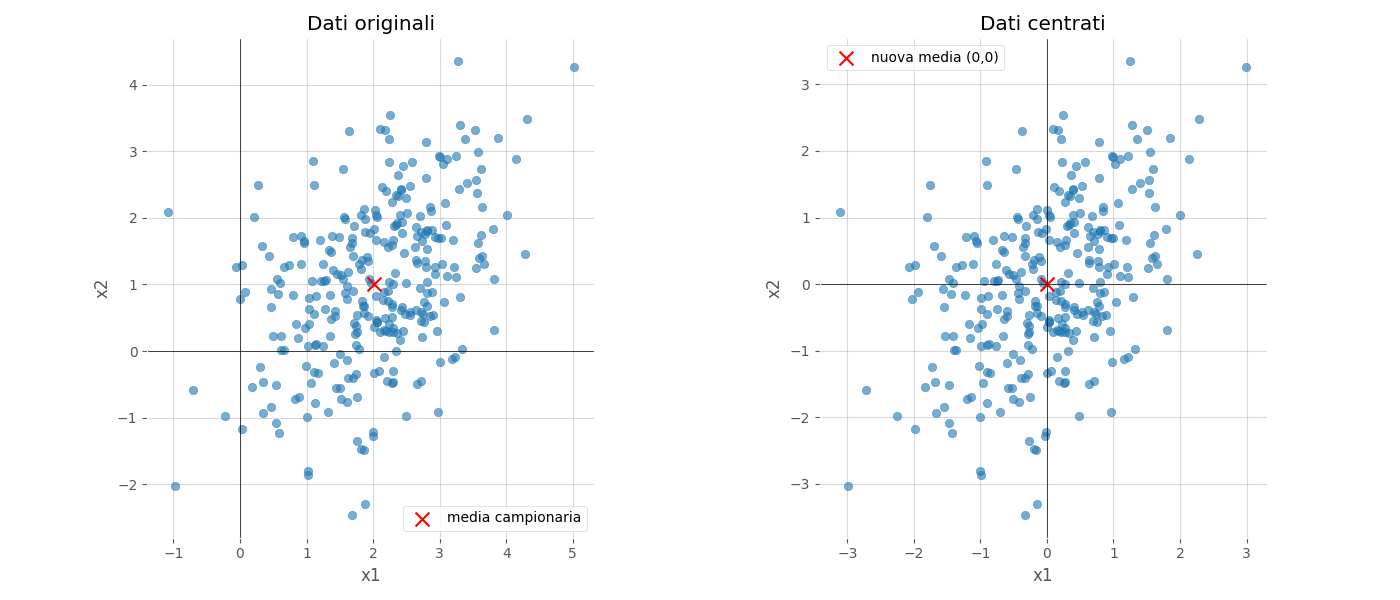
\includegraphics[width=\textwidth]{images/th_07_09/centering_transformation.png}
    \caption{Esempio di centratura di un vettore aleatorio bidimensionale. La distribuzione originale (a sinistra) viene traslata in modo che la sua media coincida con l'origine (a destra).}
    \label{fig:centering_transformation}
\end{figure}

\subsubsection{Standardizzare le Varianze}
L'obiettivo è scalare le componenti del vettore in modo che abbiano tutte
varianza unitaria (pari a 1).
\begin{itemize}
    \item \textbf{Trasformazione:} Si divide ogni componente \(X_i\) per la sua
    deviazione standard \(\text{std}(X_i)\).
    \[ Y_i = \frac{X_i}{\text{std}(X_i)} \]
    \item \textbf{Forma Matriciale:} Corrisponde a \(Y = BX\) dove \(B\) è una
    matrice diagonale contenente le inverse delle deviazioni standard:
    \[ B = \text{diag}(\text{std}(X_1)^{-1}, \dots, \text{std}(X_m)^{-1}) \]
\item \textbf{Risultato:} La matrice di covarianza del vettore trasformato \(Y\)
diventa la \textbf{matrice di correlazione} del vettore originale \(X\).
L'elemento \((i,j)\) di \(C(Y)\) è:
\[
    [C(Y)]_{ij} = \text{Cov}\left(\frac{X_i}{\text{std}(X_i)}, \frac{X_j}{\text{std}(X_j)}\right)
    \stackrel{\text{\tiny(per bilinearità della Cov)}}{=} \frac{\text{Cov}(X_i, X_j)}{\text{std}(X_i)\text{std}(X_j)}
    = \rho(X_i, X_j)
\]
\end{itemize}

\begin{figure}[H]
    \centering
    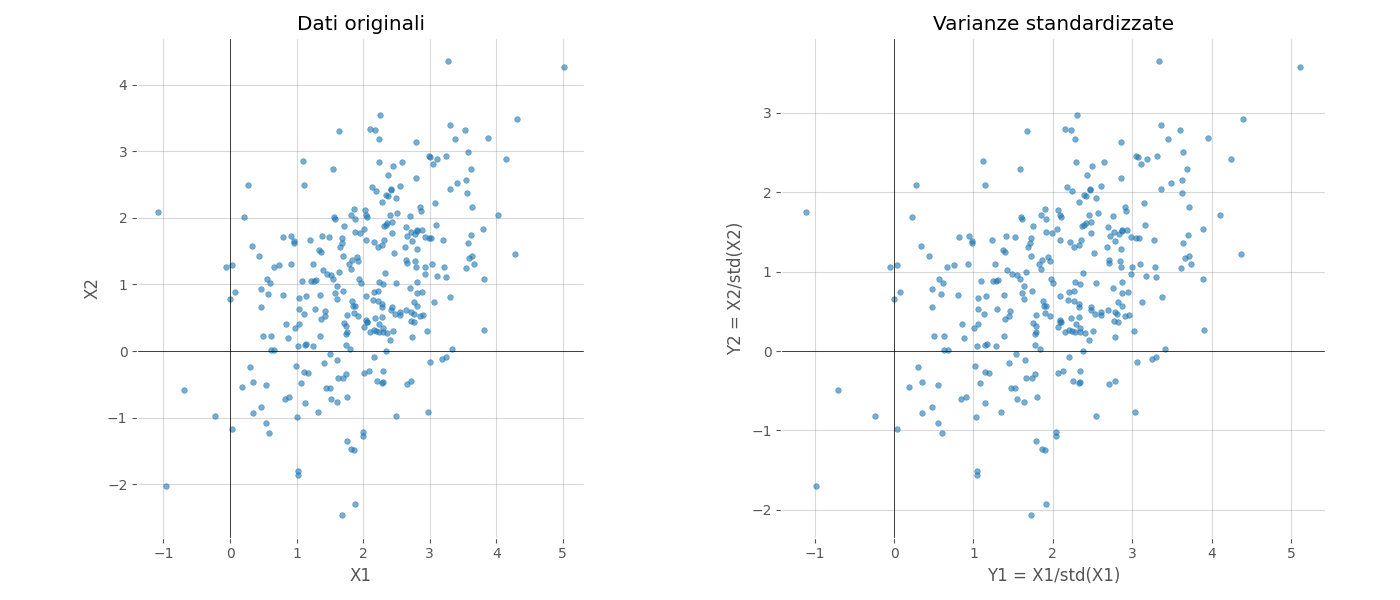
\includegraphics[width=\textwidth]{images/th_07_09/standardize_variances.png}
    \caption{Esempio di standardizzazione delle varianze di un vettore aleatorio bidimensionale. La distribuzione originale (a sinistra) viene trasformata in modo che le sue varianze siano tutte pari a 1 (a destra).}
    \label{fig:standardize_variances}
\end{figure}

\paragraph{Standardizzazione Completa (Z-score)}
Questa trasformazione combina le due precedenti per ottenere un vettore le cui
componenti hanno media 0 e varianza 1.
\begin{itemize}
    \item \textbf{Trasformazione:} È l'operazione nota come calcolo dello
    Z-score.
    \[ Y_i = \frac{X_i - E(X_i)}{\text{std}(X_i)} \]
    \item \textbf{Forma Matriciale:} Si applicano in ordine la centratura e la
    standardizzazione della varianza.
    \[ Y = \text{diag}(\text{std}(X)^{-1}) (X - \mu_X) \]
    \item \textbf{Risultato:} Il vettore trasformato \(Y\) ha media nulla e la
    sua matrice di covarianza coincide con la matrice di correlazione di \(X\).
    \[ \mu_Y = 0, \quad \Sigma_Y = \rho(X) \]
\end{itemize}

\begin{figure}[H]
    \centering
    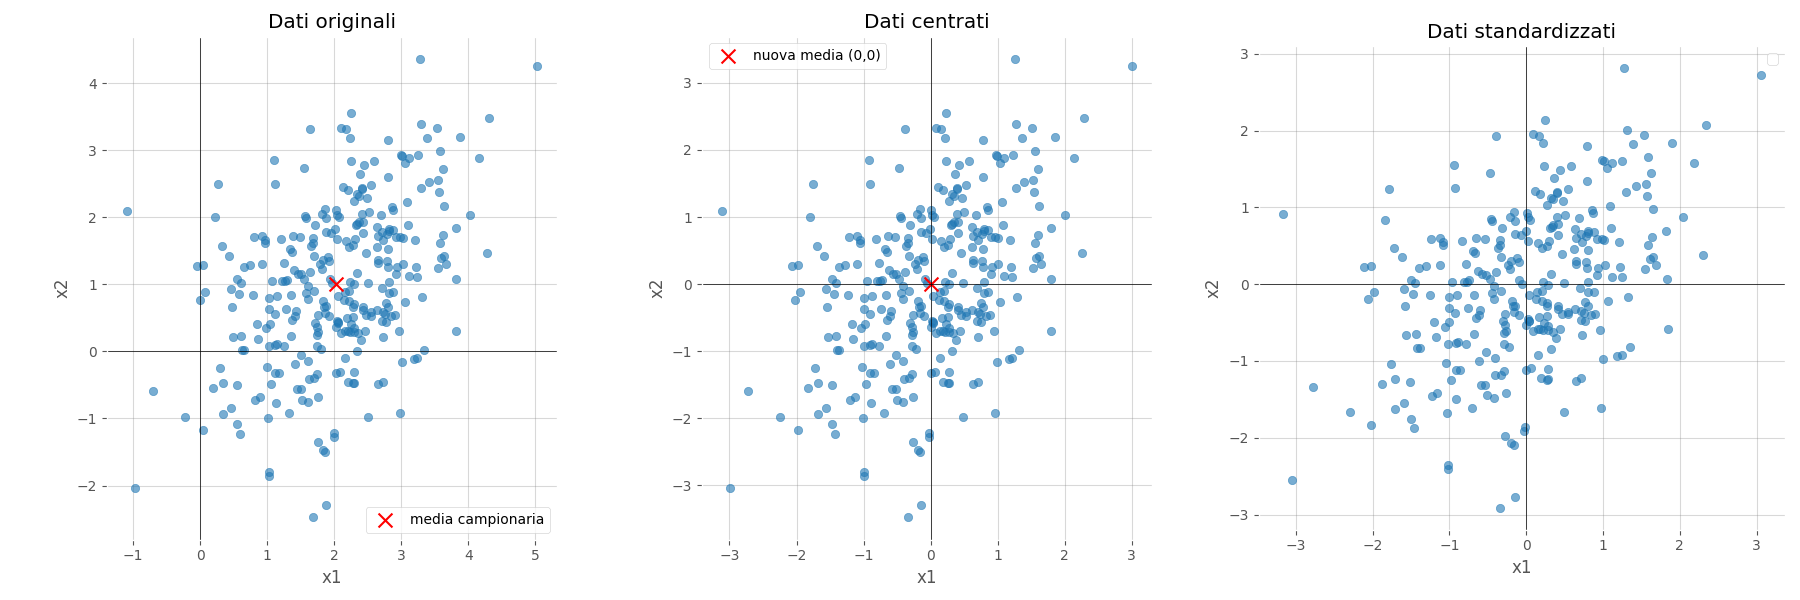
\includegraphics[width=\textwidth]{images/th_07_09/z_transformation.png}
    \caption{Esempio di standardizzazione (Z-score) di un vettore aleatorio bidimensionale. La distribuzione originale (a sinistra) viene trasformata in modo che le sue componenti abbiano media 0 (in centro) e varianza 1 (a destra).}
    \label{fig:z_transformation}
\end{figure}
\section{Principal Component Analysis (PCA)}\label{sec:pca}

\subsection{Richiami utili}

\begin{nota}{Spettro di una matrice simmetrica}{spettro}
Visto che \( \Sigma \in \mathcal{M}_{n \times n}\) è simmetrica e definita
positiva (come ogni matrice di covarianza), allora:
\begin{itemize}
  \item ammette $n$ autovalori reali e non negativi: \( \lambda_i \geq 0 \);
  \item esiste una base ortonormale di autovettori \( v_i \);
  \item gli autovettori sono ortogonali tra loro;
  \item \( \Sigma v_i = \lambda_i v_i \) equivale a dire che \( \Sigma = V
  \Lambda V^\mathsf{T} \).
\end{itemize}
\end{nota}

\subsection{Definizione}

La \textbf{Principal Component Analysis (PCA)} è una trasformazione lineare che
serve a decorrelare le componenti di un dataset multidimensionale. È
comunemente utilizzata per la riduzione della dimensionalità, il pre-processing
e la visualizzazione.

\begin{definizione}{Componenti principali}{pca}
La PCA consiste nel trovare una base ortonormale nello spazio dei dati tale che:
\begin{itemize}
  \item le nuove coordinate (\emph{componenti principali}) siano incorrelate tra
  loro;
  \item la prima componente abbia la massima varianza possibile;
  \item ogni successiva componente massimizzi la varianza residua, mantenendosi
  ortogonale alle precedenti.
\end{itemize}
\end{definizione}

\subsection{Interpretazione geometrica}

La PCA applica una \textbf{rotazione dello spazio} dei dati centrati (cioè con
media nulla), allineando gli assi principali con le direzioni di massima
varianza. Se \( X \in \mathbb{R}^{n \times d} \) è il dataset centrato:
\[
Y = V^\mathsf{T} X
\]
dove \( V \in \mathbb{R}^{d \times d} \) è la matrice degli autovettori di \(
\Sigma = \mathrm{Cov}(X) \). Le nuove variabili \( Y \) sono scorrelate e
ordinate per varianza decrescente.

\begin{figure}[H]
    \centering
    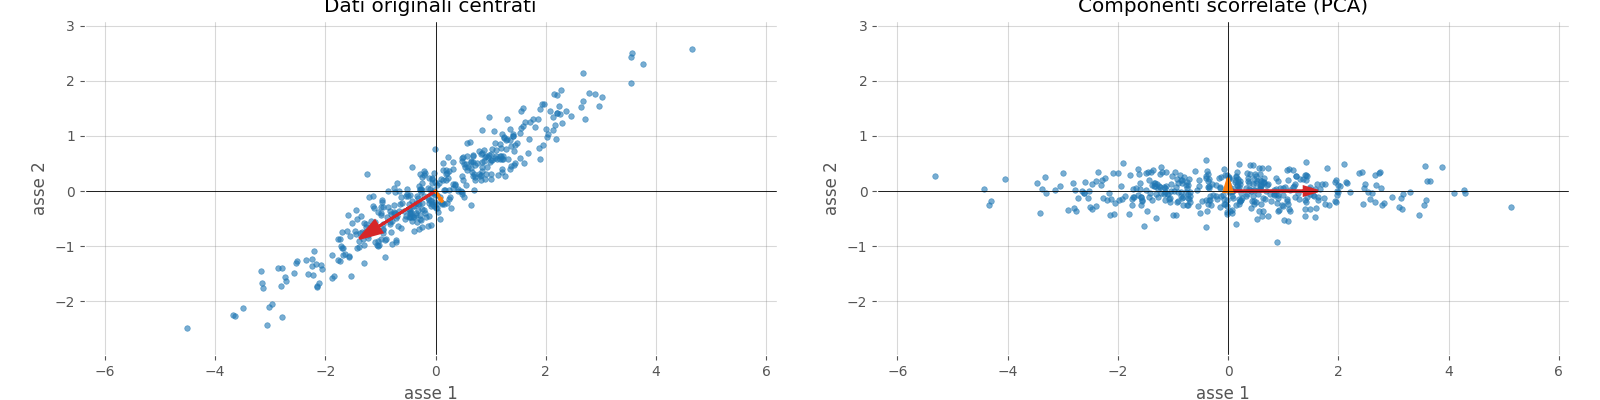
\includegraphics[width=\textwidth]{images/th_10_12/rotation_transformation.png}
    \caption{Esempio di rotazione di un vettore aleatorio bidimensionale. La distribuzione originale centrata (a sinistra) viene ruotata in modo che i suoi assi principali coincidano con le direzioni di massima varianza (a destra).}
    \label{fig:rotation_transformation}
\end{figure}

\subsection{Autovalori e autovettori della covarianza}

\begin{teorema}{Teorema spettrale per la matrice di covarianza}{pca-spettrale}
Sia \( \Sigma \in \mathbb{R}^{d \times d} \) una matrice di covarianza, cioè
reale, simmetrica e definita positiva. Allora esistono:
\begin{itemize}
  \item una base ortonormale di autovettori \( v_1, \dots, v_d \in \mathbb{R}^d
  \);
  \item autovalori reali non negativi \( \lambda_1, \dots, \lambda_d \geq 0 \);
\end{itemize}
tali che:
\[
\Sigma v_k = \lambda_k v_k, \qquad v_j^\mathsf{T} v_k = \delta_{jk}
\]
cioè:
\[
\Sigma = V \Lambda V^\mathsf{T}
\]
dove \( V = [v_1 \; \dots \; v_d] \) è ortogonale e \( \Lambda =
\mathrm{diag}(\lambda_1, \dots, \lambda_d) \).
\end{teorema}

\begin{proposizione}{La matrice degli autovettori è
ortogonale}{pca-matrice-ortogonale}
Sia \( \Sigma \in \mathbb{R}^{d \times d} \) una matrice simmetrica. Siano \(
v_1, \dots, v_d \in \mathbb{R}^d \) autovettori ortonormali di \( \Sigma \), e
si definisca \( V := [v_1 \ \dots \ v_d] \in \mathbb{R}^{d \times d} \). Allora:
\[
V^\mathsf{T} V = I \quad \text{e} \quad VV^\mathsf{T} = I
\]
cioè \( V \) è una matrice ortogonale.
\end{proposizione}

\begin{dimostrazione}{}{dim-pca-matrice-ortogonale}
Osserviamo che l’elemento \( (i, j) \) della matrice \( V^\mathsf{T} V \) si
calcola come:
\[
[V^\mathsf{T} V]_{ij} = \sum_{k=1}^d [V^\mathsf{T}]_{ik} [V]_{kj}
= \sum_{k=1}^d v_{k,i} v_{k,j}
\]

Notiamo che:
\[
\sum_{k=1}^d v_{k,i} v_{k,j} = v_i^\mathsf{T} v_j =
\begin{cases}
1 & \text{se } i = j \\
0 & \text{se } i \neq j
\end{cases}
= \delta_{ij}
\]

Quindi:
\[
V^\mathsf{T} V = I \quad \text{(matrice identità)}
\]

Segue che \( V \) è ortogonale, quindi \( V^\mathsf{T} = V^{-1} \).
Da questo deduciamo anche \( VV^\mathsf{T} = I \), e quindi:
\[
VV^\mathsf{T} = V V^{-1} = I
\]

In conclusione, \( V \) è una rotazione (o riflessione), cioè una
trasformazione ortogonale dello spazio.
\end{dimostrazione}

\begin{proposizione}{Diagonalizzazione spettrale: \texorpdfstring{\( \Sigma V =
V \Lambda \)}{Sigma V = V Lambda}}{pca-spettrale-diretta}
Sia \( \Sigma \in \mathbb{R}^{d \times d} \) una matrice simmetrica, e siano \(
v_1, \dots, v_d \) i suoi autovettori ortonormali associati agli autovalori \(
\lambda_1, \dots, \lambda_d \). Costruiamo:
\[
V := [v_1 \; v_2 \; \dots \; v_d], \quad \Lambda := \mathrm{diag}(\lambda_1,
\dots, \lambda_d)
\]
Allora:
\[
\Sigma V = V \Lambda
\]
\end{proposizione}

\begin{dimostrazione}{}{dim-pca-spettrale-diretta}
    \paragraph{Versione vista a lezione} Verifichiamo che \( \Sigma V = V
    \Lambda \) calcolando il generico elemento \( (i, j) \) di entrambi i
    membri.

A sinistra:
\[
[\Sigma V]_{ij} = \sum_k \Sigma_{ik} V_{kj}
= \sum_k \Sigma_{ik} (v_j)_k = [\Sigma v_j]_i
\]
Poiché \( v_j \) è autovettore di \( \Sigma \), abbiamo:
\[
\Sigma v_j = \lambda_j v_j \quad \Rightarrow \quad [\Sigma v_j]_i = \lambda_j
(v_j)_i = \lambda_j V_{ij}
\]

A destra:
\[
[V \Lambda]_{ij} = \sum_k V_{ik} \Lambda_{kj} = V_{ij} \lambda_j = \lambda_j
V_{ij}
\]

Poiché i due membri coincidono elemento per elemento:
\[
    [V \Lambda]_{ij} = \sum_k V_{ik} \Lambda_{kj} \stackrel{\text{\tiny
    (\(\Lambda_{kj} = 0 \forall k \neq j\))}}{=} V_{ij} \lambda_j = \lambda_j
    V_{ij}
\]

\paragraph{Alternativa}

Abbiamo già verificato che:
\[
\Sigma = V \Lambda V^\mathsf{T} ,\quad V^\mathsf{T}V = VV^\mathsf{T} = I
\]
Moltiplicando ambo i membri della prima equazione per $V$ otteniamo:
\begin{align*}
    \Sigma &= V \Lambda V^\mathsf{T} \\
    \Sigma V &= V \Lambda (V^\mathsf{T} V) \\
    \Sigma V &= V \Lambda
\end{align*}

\end{dimostrazione}

\subsection{PCA e decorrelazione}

\begin{proposizione}{Decorrelazione delle componenti tramite
PCA}{pca-covarianza-diagonale}
Sia \( X \in \mathbb{R}^{d \times n} \) un dataset centrato con matrice di
covarianza \( \Sigma = \mathrm{Cov}(X) \). Sia \( V \in \mathbb{R}^{d \times d}
\) una matrice ortogonale composta dagli autovettori di \( \Sigma \), e sia:
\[
Y = V^\mathsf{T} X
\]
la trasformazione PCA. Allora:
\[
\mathrm{Cov}(Y) = \Lambda
\]
dove \( \Lambda \) è la matrice diagonale degli autovalori di \( \Sigma \).
\end{proposizione}

\begin{dimostrazione}{}{dim-pca-covarianza-diagonale}
Poiché \( Y = V^\mathsf{T} X \), la matrice di covarianza di \( Y \) è:
\[
\mathrm{Cov}(Y) = \mathrm{Cov}(V^\mathsf{T} X)
\]

Usando la \Cref{prop:cov_trasformata} sulla variazione della covarianza in una
trasformazione lineare otteniamo:
\[
    \mathrm{Cov}(Y)
    = V^\mathsf{T} \, \Sigma \, (V^\mathsf{T})^\mathsf{T}
    = V^\mathsf{T} \Sigma V
\]

Poiché \( \Sigma = V \Lambda V^\mathsf{T} \), allora:
\[
\mathrm{Cov}(Y) = V^\mathsf{T} (V \Lambda V^\mathsf{T}) V = (V^\mathsf{T} V)
\Lambda (V^\mathsf{T} V) = I \Lambda I = \Lambda
\]

Quindi \( \mathrm{Cov}(Y) \) è diagonale e coincide con la matrice degli
autovalori di \( \Sigma \), cioè le varianze delle componenti principali.
\end{dimostrazione}

\subsection{Scelte pratiche nella PCA: standardizzazione o no?}

\paragraph{Due approcci standard alla PCA.}
Ci sono due modalità comuni per eseguire la PCA:

\begin{enumerate}
  \item Centrare i dati rispetto alla media, poi eseguire la PCA sulla matrice
  di covarianza \( \Sigma = \mathrm{Cov}(X) \) e infine standardizzare (Vedi
  immagine \ref{fig:pca_progressione1}).
  \item Centrare i dati rispetto alla media, standardizzare ogni variabile
  (cioè trasformarla in una variabile con media 0 e varianza 1), poi fare la
  PCA sulla matrice di correlazione ed eventualmente standardizzare di nuovo
  subito dopo. (Vedi
  immagine \ref{fig:pca_progressione2}).
\end{enumerate}

\begin{figure}[H]
    \centering
    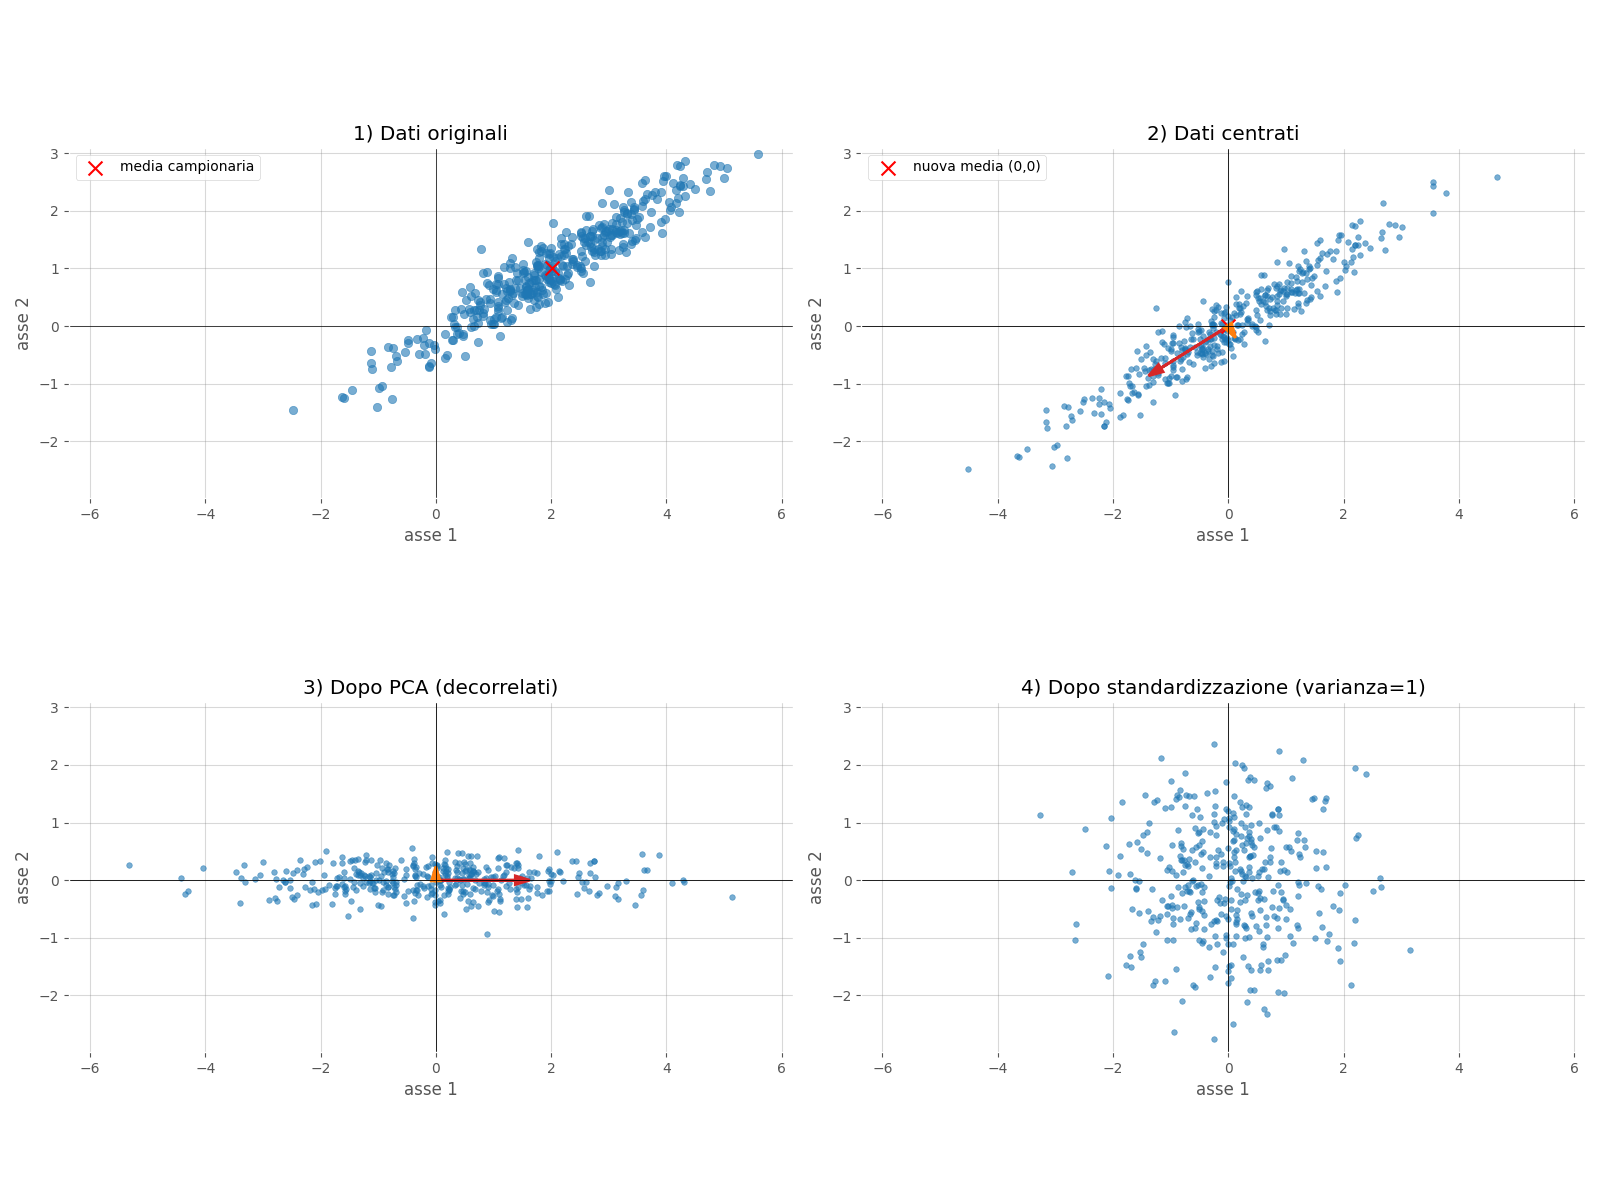
\includegraphics[width=\textwidth]{images/th_10_12/pca_progressione1.png}
    \caption{Esempio di primo approccio alla PCA: 1) Dati originali. 2) Dati centrati. 3) PCA. 4) Dati standardizzati dopo la PCA.}
    \label{fig:pca_progressione1}
\end{figure}

\begin{figure}[H]
    \centering
    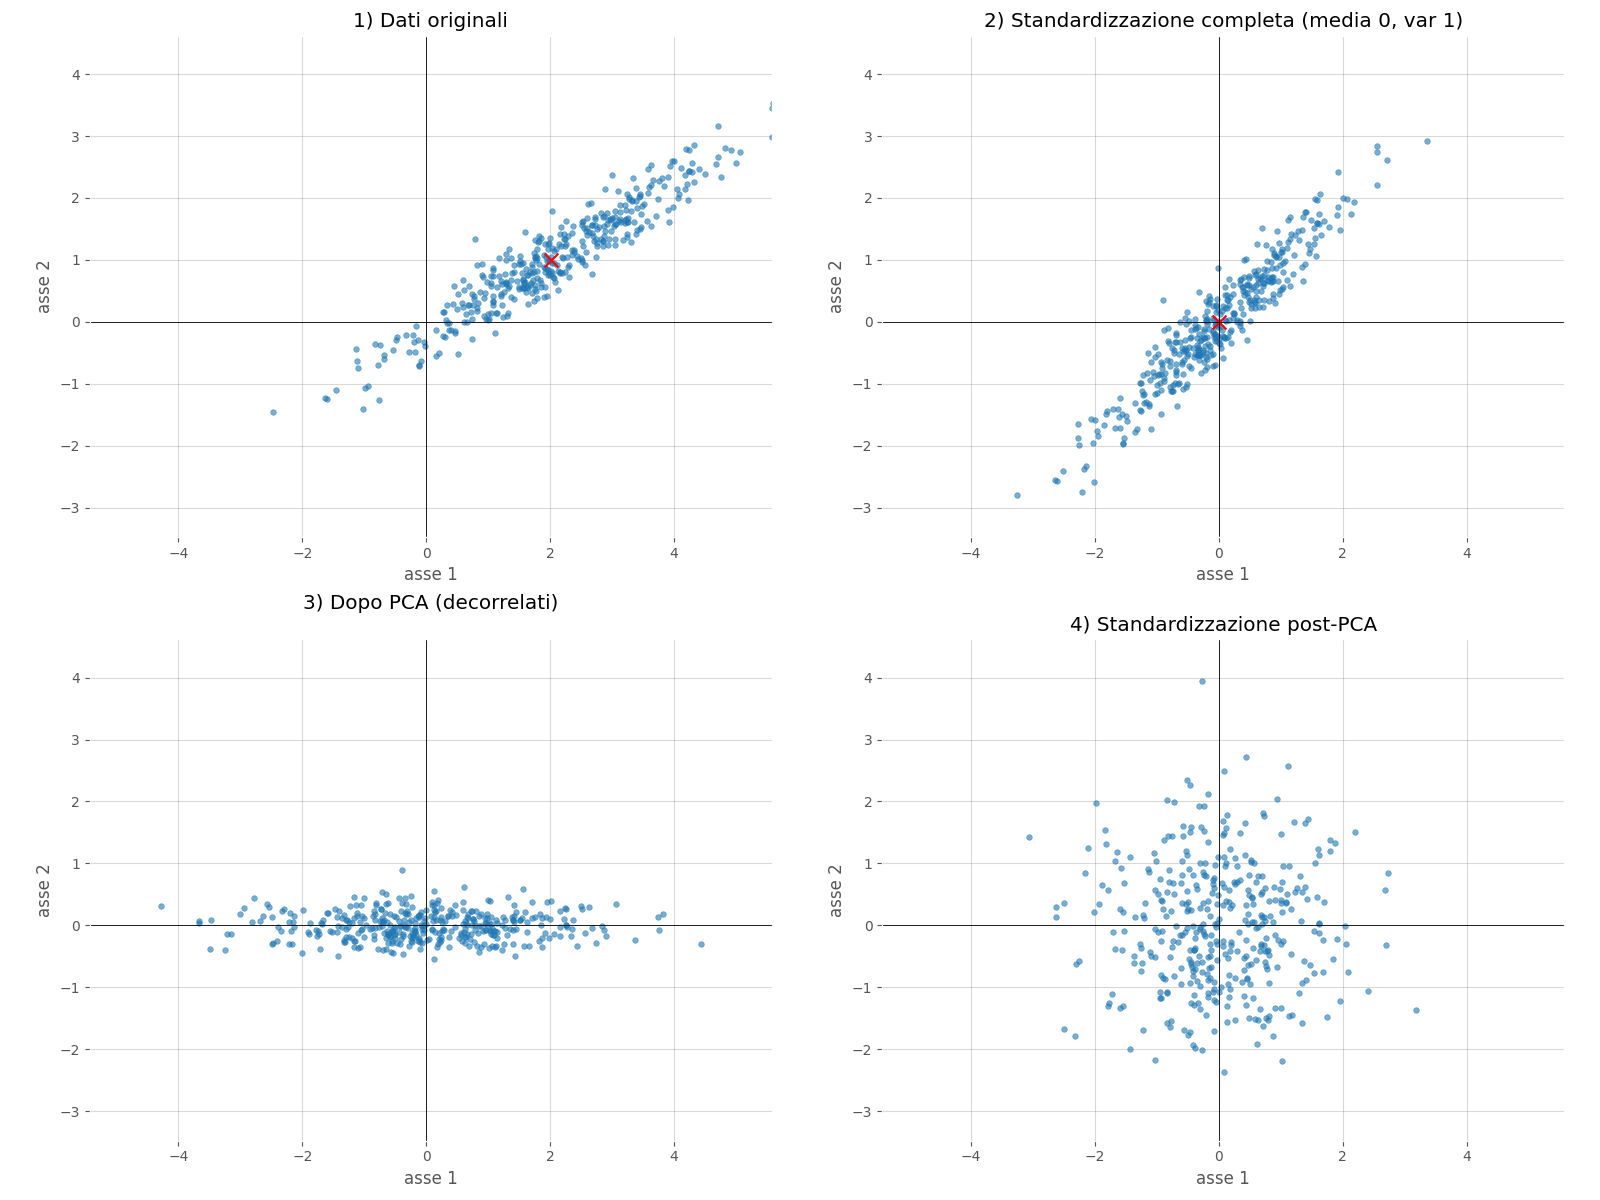
\includegraphics[width=\textwidth]{images/th_10_12/pca_progressione2.png}
    \caption{Esempio di secondo approccio alla PCA: 1) Dati originali. 2) Standardizzazione completa. 3) PCA. 4) Dati standardizzati dopo la PCA.}
    \label{fig:pca_progressione2}
\end{figure}

Questi due approcci corrispondono a:

\begin{itemize}
  \item PCA su \( \Sigma \): privilegia le direzioni di massima varianza
  assoluta;
  \item PCA su matrice di correlazione: privilegia le direzioni di massima
  varianza relativa, indipendente dall'unità di misura.
\end{itemize}

\begin{nota}{Approccio standardizzato}{pca-standard}
Applicare la PCA dopo aver standardizzato equivale a diagonalizzare la matrice
di correlazione \( \rho(X) \), ovvero \( \mathrm{Cov}(Z) \) dove \( Z \) è la
versione standardizzata di \( X \).
\end{nota}

\paragraph{Unità di misura e varianza.}
La matrice di covarianza \( \Sigma = \mathrm{Cov}(X) \) è influenzata
dall’unità di misura delle variabili: se una variabile ha un’unità molto
più grande, avrà anche una varianza più grande, e quindi tenderà a dominare
le componenti principali.

\begin{nota}{Influenza delle unità di misura}{pca-unita}
Se le variabili hanno unità di misura molto diverse (es. altezza in cm, peso in
kg), conviene standardizzare prima della PCA. Altrimenti la componente
principale potrebbe riflettere solo la scala di una variabile.
\end{nota}

\paragraph{Rappresentazione grafica dei due approcci.}

Nella seconda riga viene applicata la standardizzazione prima della PCA: il
risultato finale (dopo PCA) è visivamente diverso. In entrambi i casi si
ottiene una matrice di covarianza diagonale, ma le componenti principali sono
diverse.

\begin{nota}{Quando usare la standardizzazione}{pca-standard-when}
Se non si ha una chiara ragione per dare peso a una variabile più che ad
un'altra (es. tutte hanno importanza comparabile), allora è consigliabile usare
l'approccio con standardizzazione.
\end{nota}



\section{Analisi Fattoriale (Factor Analysis)}\label{sec:factor-analysis}

L'Analisi Fattoriale è una tecnica statistica utilizzata per ridurre il numero
di variabili osservate in un numero inferiore di variabili latenti chiamate
\textbf{fattori}. Mentre la PCA riduce la dimensionalità conservando la
varianza, la Factor Analysis cerca di spiegare le correlazioni tra le variabili
attraverso fattori latenti, e può essere vista come un'estensione della PCA.

\begin{definizione}{Fattori e variabili osservate}{factor-analysis}
Nel modello di Analisi Fattoriale, le variabili osservate \( X_1, X_2, \dots,
X_m \) sono espresse come una combinazione lineare di fattori latenti \( F_1,
F_2, \dots, F_k \) più un errore \( \epsilon_1, \epsilon_2, \dots, \epsilon_m
\):
\[
X_i = \lambda_{i1} F_1 + \lambda_{i2} F_2 + \dots + \lambda_{ik} F_k +
\epsilon_i
\]
dove \( \lambda_{ij} \) è il \textbf{factor loading} che esprime la relazione
tra la variabile osservata \( X_i \) e il fattore \( F_j \).
\end{definizione}

\subsection{Factor Loadings}

I \textbf{factor loadings} \( \lambda_{ij} \) rappresentano il peso di ciascun
fattore latente \( F_j \) sulla variabile osservata \( X_i \). Questi valori
mostrano quanto ciascun fattore contribuisce alla varianza della variabile
osservata. Un alto factor loading indica che la variabile è fortemente
correlata con il fattore.

\begin{esempio}{Factor loadings}{factor-loadings}
Nel caso di due fattori latenti \( F_1 \) e \( F_2 \), i fattori di carico
potrebbero essere:
\[
F_1 = 1.1 X_1 + 0.8 X_2, \quad F_2 = 1.1 X_1 + 0.8 X_2
\]
Ciò significa che \( X_1 \) e \( X_2 \) sono fortemente influenzati da entrambi
i fattori, con pesi \( \lambda_{11} = 1.1 \), \( \lambda_{12} = 0.8 \), e così
via.
\end{esempio}

\subsection{Obiettivo dell'analisi fattoriale}

L'obiettivo dell'Analisi Fattoriale è quello di ridurre il numero di variabili
osservate \( X_1, X_2, \dots, X_m \) in \( k \) fattori \( F_1, F_2, \dots, F_k
\), dove \( k < m \), cercando di mantenere la maggior parte della varianza.
L'analisi si concentra nel trovare i fattori latenti che meglio spiegano le
correlazioni tra le variabili.

\begin{nota}{Riduzione dimensionale nella Factor Analysis}{factor-reduction}
La riduzione di dimensione in Factor Analysis non è come nella PCA, dove si
cerca di massimizzare la varianza, ma si cerca di spiegare le correlazioni tra
le variabili attraverso un numero ridotto di fattori.
\end{nota}

\subsection{Quando usare l'Analisi Fattoriale?}

L'Analisi Fattoriale è utile quando:
\begin{itemize}
  \item Le variabili originali sono fortemente correlate tra loro;
  \item Si vuole ridurre la dimensionalità dei dati senza perdere troppe
  informazioni;
  \item Le variabili sono influenzate da un numero ridotto di fattori latenti.
\end{itemize}

\begin{nota}{Fattori "schiacciati"}{factor-schiacciati}
Quando il numero di variabili osservate \( m \) è grande e ci sono molte
componenti di \( Y \) con varianza piccola, l'Analisi Fattoriale è spesso più
adatta rispetto alla PCA, che potrebbe perdere troppe informazioni in presenza
di molte variabili "schiacciate" (ovvero con bassa varianza).
\end{nota}

\subsection{Relazione con la PCA}

L'Analisi Fattoriale può essere vista come una generalizzazione della PCA.
Mentre la PCA si concentra nel massimizzare la varianza, la Factor Analysis
cerca di spiegare la varianza condivisa tra le variabili attraverso fattori
latenti. Quindi, la PCA può essere considerata come un caso particolare di
Factor Analysis, dove tutti i fattori sono assunti ortogonali e indipendenti.

\subsection{Riduzione dimensionale e scelta del numero di componenti}

Quando \( m \) (il numero di variabili) è grande, esistono molte componenti
principali con varianza piccola. La PCA cerca di ridurre la dimensione del
vettore \( X \) mantenendo la varianza totale e riducendo la complessità del
modello. La somma delle varianze prima e dopo la trasformazione è costante e
conserva la varianza totale:
\[
\text{Var}(X_1) + \dots + \text{Var}(X_m) = \text{Var}(Y_1) + \dots +
\text{Var}(Y_m) = \text{varianza totale}
\]
Questa relazione implica che la traccia della matrice di covarianza \( \Sigma \)
è uguale alla somma degli autovalori di \( \Sigma \), ovvero:
\[
\text{tr}(\Sigma) = \text{tr}(\Lambda)
\]
dove \( \Lambda \) è la matrice diagonale degli autovalori.

\subsubsection{Distribuzione degli autovalori}

Tipicamente, gli autovalori \( \lambda_1 \geq \lambda_2 \geq \dots \geq
\lambda_m > 0 \) sono ordinati in modo decrescente. Questo ordine riflette la
quantità di varianza spiegata da ciascuna componente principale. I componenti
principali con autovalori maggiori spiegano una porzione maggiore della varianza
totale.

Un approccio comune è quello di utilizzare un grafico dei cosiddetti
\textbf{cambiamenti di pendenza} (come lo scree plot \ref{fig:screeplot}) per determinare il numero
di componenti principali da mantenere. Un cambiamento significativo nella
pendenza suggerisce il numero ottimale di componenti da considerare:
Nel grafico sopra, le prime 3 componenti sembrano spiegare la maggior parte
della varianza.

\begin{figure}[H]
    \centering
    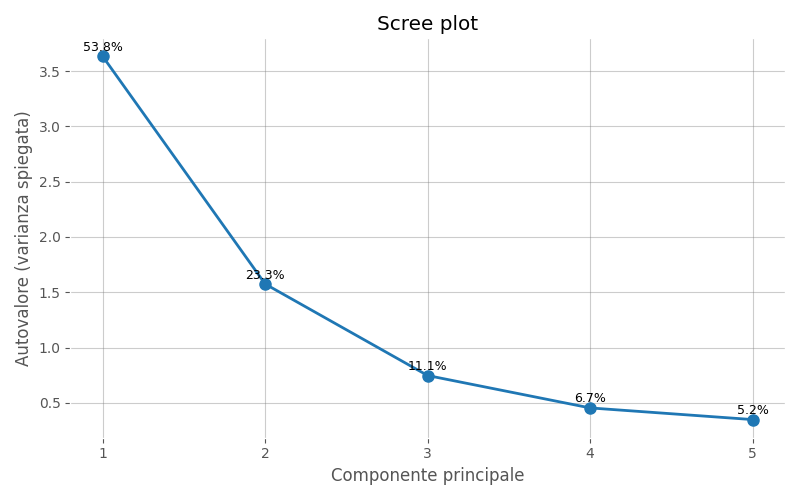
\includegraphics[width=0.6\textwidth]{images/th_10_12/screeplot.png}
    \caption{Esempio di scree plot per la selezione del numero di componenti principali. Si osserva un cambiamento di pendenza significativo dopo la terza componente, suggerendo che le prime tre componenti catturano la maggior parte della varianza.}
    \label{fig:screeplot}
\end{figure}

\subsection{Quando standardizzare i dati}

Quando i dati hanno unità di misura diverse, è importante standardizzarli
prima di applicare la PCA. Questo è cruciale, poiché le variabili con unità
più grandi tenderanno a dominare la varianza, influenzando fortemente le
componenti principali.

Se dopo la PCA i dati non vengono standardizzati, si ottiene una rotazione dei
dati senza alcuna scalatura. In questo caso, la PCA non fornirà una riduzione
della dimensione che tiene conto della varianza relativa di ciascuna variabile,
ma solo una rotazione rispetto alla distribuzione dei dati. Di conseguenza, la
distanza tra i punti sarà influenzata solo dalla loro distribuzione e non dalla
varianza delle variabili.

\begin{nota}{Standardizzazione dopo PCA}{pca-standardizzazione}
Standardizzare i dati prima della PCA è fondamentale per ridurre il rischio di
amplificare il rumore nelle componenti con bassa varianza. La standardizzazione
aiuta a bilanciare l'influenza di variabili con scale diverse.
\end{nota}

\subsection{Effetto della standardizzazione}

Quando i dati vengono standardizzati dopo la PCA, la varianza di ciascuna
componente principale è distribuita in modo più uniforme, evitando che
variabili con bassa varianza distorcano i risultati. Il grafico sottostante
mostra l'effetto della standardizzazione:

Nel grafico:
- \( \mu \) e \( \Sigma \) indicano i dati originali con la loro media e
covarianza,
- \( 0, \Sigma \) indica i dati centrati ma non standardizzati,
- \( 0, I \) rappresenta i dati dopo standardizzazione.

\begin{nota}{Importanza della standardizzazione}{pca-scaling}
La standardizzazione dopo la PCA è essenziale quando le variabili hanno scale
diverse, poiché permette una comparazione equa tra le variabili e riduce
l'influenza di quelle con una varianza maggiore.
\end{nota}

\section{Distribuzioni Multidimensionali Notevoli}

\subsection{Distribuzione Gaussiana Multidimensionale}

La distribuzione Gaussiana (o Normale) Multidimensionale è una delle
distribuzioni di probabilità più importanti in statistica e machine learning.
Essa rappresenta la generalizzazione della distribuzione Gaussiana a vettori
aleatori di più dimensioni.

\begin{definizione}{Gaussiana Multidimensionale}{gaussiana-multi}
Un vettore aleatorio $X = (X_1, X_2, \dots, X_p)$ a valori in $\mathbb{R}^p$
segue una distribuzione Gaussiana Multidimensionale se la sua notazione è
$$
X \sim \mathcal{N}(\mu, \Sigma)
$$
dove:
\begin{itemize}
    \item $\mu \in \mathbb{R}^p$ è il \textbf{vettore media}.
    \item $\Sigma \in M_{p,p}$ è la \textbf{matrice di covarianza}, che deve
    essere simmetrica e semidefinita positiva.
\end{itemize}
\end{definizione}

\begin{nota}{}{gaussiana-params}
I parametri $\mu$ e $\Sigma$ determinano completamente la distribuzione. Il
vettore media $\mu$ definisce il centro della distribuzione, mentre la matrice
di covarianza $\Sigma$ ne definisce la forma e l'orientamento.
\end{nota}

Geometricamente, per $p=2$, la funzione di densità di probabilità (PDF) ha una
forma a campana tridimensionale. Le curve di livello di questa campana sono
ellissi concentriche centrate in $\mu$.

\begin{figure}[H]
    \centering
    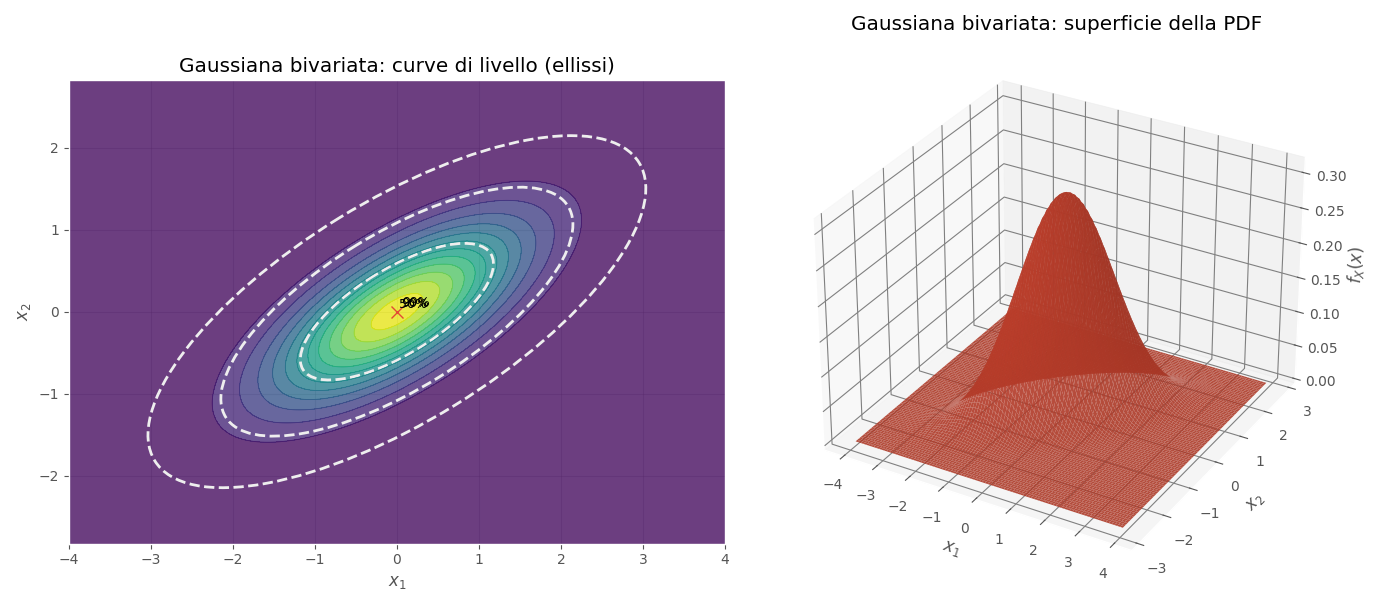
\includegraphics[width=0.6\textwidth]{images/th_10_12/gaussiana_multidimensionale_2d3d.png}
    \caption{Esempio di distribuzione Gaussiana bivariata con media $\mu$ e matrice di covarianza $\Sigma$. Le curve di livello sono ellissi che rappresentano le regioni di uguale densità di probabilità.}
    \label{fig:gaussiana_bivariata}
\end{figure}

\begin{proposizione}{Funzione di Densità di Probabilità (PDF)}{gaussiana-pdf}
Se la matrice di covarianza $\Sigma$ è invertibile (ovvero definita positiva),
allora il vettore aleatorio $X$ ammette una funzione di densità di probabilità
$f_X(x)$ data da:
$$
f_X(x) = \frac{1}{(2\pi)^{p/2} \det(\Sigma)^{1/2}}
\exp\left\{-\frac{1}{2}(x-\mu)^T \Sigma^{-1} (x-\mu)\right\}
$$
Se $\Sigma$ non è invertibile (singolare), la distribuzione è detta
\textbf{degenere} e la massa di probabilità è concentrata su un sottospazio
affine di $\mathbb{R}^p$.
\end{proposizione}

\subsubsection*{Interpretazione della Matrice di Covarianza}

La forma e l'orientamento degli ellissoidi delle curve di livello dipendono
direttamente dalla matrice di covarianza $\Sigma$.

\begin{nota}{}{gaussiana-cov-assi}
Una covarianza nulla tra due componenti, $\text{Cov}(X_i, X_j) = \Sigma_{ij} =
0$, implica che gli assi degli ellissoidi sono paralleli agli assi cartesiani.
\end{nota}

\begin{esempio}{Forma degli Ellissoidi}{gaussiana-ellissoidi}
Analizziamo tre casi per una Gaussiana bivariata ($p=2$) con media $\mu =
\begin{pmatrix} 0 \\ 0 \end{pmatrix}$:
\begin{enumerate}
    \item[\textbf{a.}] \textbf{Covarianza nulla:} Se $\Sigma = \begin{pmatrix}
    \sigma_1^2 & 0 \\ 0 & \sigma_2^2 \end{pmatrix}$, ad esempio $\Sigma =
    \begin{pmatrix} 2 & 0 \\ 0 & 1 \end{pmatrix}$, le componenti $X_1$ e $X_2$
    sono incorrelate. Gli assi degli ellissoidi sono allineati con gli assi
    cartesiani e la loro larghezza è proporzionale a $\sigma_1$ e $\sigma_2$.
    
    \item[\textbf{b.}] \textbf{Covarianza non nulla:} Se $\Sigma =
    \begin{pmatrix} 2 & 1 \\ 1 & 1 \end{pmatrix}$, la covarianza non nulla
    $\Sigma_{12}=1$ indica una correlazione tra $X_1$ e $X_2$. Questo causa una
    rotazione degli ellissoidi: i loro assi principali non sono più paralleli
    agli assi cartesiani.
    
    \item[\textbf{c.}] \textbf{Matrice singolare (degenere):}] Se $\Sigma =
    \begin{pmatrix} 2 & \sqrt{2} \\ \sqrt{2} & 1 \end{pmatrix}$, la matrice non
    è invertibile ($\det(\Sigma) = 2 \cdot 1 - (\sqrt{2})^2 = 0$). Tutta la
    massa di probabilità giace sulla retta $x_1 = \sqrt{2} x_2$. La
    distribuzione non ha una PDF in $\mathbb{R}^2$.
\end{enumerate}
\end{esempio}

Una proprietà fondamentale e unica della distribuzione Gaussiana riguarda la
relazione tra indipendenza e incorrelazione.

\begin{teorema}{Indipendenza e Incorrelazione}{gaussiana-indip-incor}
Per un vettore aleatorio con distribuzione Gaussiana, la condizione di
\textbf{indipendenza} tra le sue componenti è \textbf{equivalente} alla
condizione di \textbf{covarianza nulla} (incorrelazione).
$$
\text{Componenti indipendenti} \iff \text{Covarianza nulla}
$$
\end{teorema}

\begin{nota}{}{gaussiana-indip-impl}
In generale, per altre distribuzioni, vale solo l'implicazione: indipendenza
$\Rightarrow$ covarianza nulla. L'implicazione inversa non è garantita, ma lo
è per la Gaussiana.
\end{nota}

\subsubsection*{Casi Particolari}

\begin{proposizione}{Gaussiana Standard Multidimensionale}{gaussiana-standard}
Se $\mu = \mathbf{0}$ e $\Sigma = I$ (matrice identità), allora le componenti
$X_1, \dots, X_p$ sono Gaussiane standard indipendenti e identicamente
distribuite, $X_i \sim \mathcal{N}(0,1)$ i.i.d.
In questo caso, la PDF ha \textbf{simmetria sferica} (o radiale):
$$
f_X(x) = (2\pi)^{-p/2} \exp\left\{-\frac{1}{2}x^T x\right\} = C \cdot
\exp\left\{-\frac{1}{2}\|x\|^2\right\}
$$
dove $\|x\|^2 = x_1^2 + \dots + x_p^2$ è il quadrato della norma euclidea.
\end{proposizione}

Una conseguenza interessante di questo caso è che la somma dei quadrati di
variabili normali standard indipendenti segue una distribuzione Chi-quadrato.

\begin{nota}{Distribuzione Chi-quadrato}{chi-quadro}
Nel caso di una Gaussiana Standard Multidimensionale, la norma quadra del
vettore $X$, $\|X\|^2$, segue una distribuzione Chi-quadrato con $p$ gradi di
libertà:
$$
\|X\|^2 \sim \chi^2(p)
$$
\end{nota}

Infine, presentiamo una definizione più astratta ma generale, che copre anche i
casi degeneri.

\begin{definizione}{Definizione Astratta}{gaussiana-astratta}
Un vettore aleatorio $X$ ha una legge Gaussiana multivariata in $\mathbb{R}^p$
se e solo se, per ogni vettore $a \in \mathbb{R}^p$, la combinazione lineare $Y
= a^T X$ ha una legge Gaussiana univariata su $\mathbb{R}$ o è una costante
deterministica.
\end{definizione}

\subsection{Distribuzione Multinomiale}

La distribuzione multinomiale è la generalizzazione della distribuzione
binomiale. Mentre un esperimento binomiale consiste in $n$ prove indipendenti
con due possibili esiti (successo/insuccesso), un esperimento multinomiale
consiste in $n$ prove indipendenti, ciascuna con $m$ possibili esiti.

\begin{definizione}{Multinomiale}{multinomiale}
Un vettore aleatorio $X = (X_1, X_2, \dots, X_m)$ segue una distribuzione
Multinomiale con parametri $n$ (numero di prove) e $p$ (vettore di
probabilità), e si scrive:
$$
X \sim \text{Multin}(n, p)
$$
dove:
\begin{itemize}
    \item $X_i$ conta il numero di volte che si è verificato l'esito $i$ nelle
    $n$ prove.
    \item $p = (p_1, p_2, \dots, p_m)$ è un vettore di probabilità, con $p_i$
    che rappresenta la probabilità dell'esito $i$.
\end{itemize}
Devono valere i seguenti vincoli: $\sum_{i=1}^{m} p_i = 1$ e $\sum_{i=1}^{m} X_i
= n$.
\end{definizione}

\begin{nota}{}{multinomiale-dipendenza}
Le componenti del vettore $X = (X_1, \dots, X_m)$ sono \textbf{dipendenti},
poiché la loro somma è fissata a $n$. Tuttavia, la distribuzione marginale di
ogni singola componente $X_i$ è una binomiale: $X_i \sim \text{Bin}(n, p_i)$.
\end{nota}

\begin{proposizione}{Funzione di Massa di Probabilità (PMF)}{multinomiale-pmf}
La funzione di massa di probabilità (PMF) della distribuzione multinomiale è
data da:
$$
P(X_1=x_1, \dots, X_m=x_m) = \frac{n!}{x_1! x_2! \dots x_m!} p_1^{x_1} p_2^{x_2}
\dots p_m^{x_m}
$$
dove $\sum_{i=1}^{m} x_i = n$. Il termine frazionario è noto come
\textbf{coefficiente multinomiale} e conta il numero di modi in cui $n$ oggetti
possono essere partizionati in $m$ gruppi di numerosità $x_1, \dots, x_m$.
\end{proposizione}

\begin{esempio}{Coefficiente Multinomiale}{multinomiale-coeff}
Quanti sono gli anagrammi della parola "STATISTICA"?
La parola è lunga $n=10$ caratteri. Le frequenze delle lettere sono: S (2), T
(3), A (2), I (2), C (1).
Il numero di anagrammi è dato dal coefficiente multinomiale:
$$
\binom{10}{2, 3, 2, 2, 1} = \frac{10!}{2! \cdot 3! \cdot 2! \cdot 2! \cdot 1!} =
75600
$$
\end{esempio}


\subsection{Distribuzione di Dirichlet}

La distribuzione di Dirichlet è una distribuzione di probabilità continua per
un vettore di numeri reali positivi che sommano a 1. È spesso descritta come
una "distribuzione su distribuzioni", ed è il coniugato a priori della
distribuzione Multinomiale nell'inferenza Bayesiana.

\begin{definizione}{Dirichlet}{dirichlet}
Un vettore aleatorio $X = (X_1, \dots, X_m)$ a valori in $\mathbb{R}^m$ segue
una distribuzione di Dirichlet con parametro di concentrazione $\alpha =
(\alpha_1, \dots, \alpha_m)$, con $\alpha_i > 0$. Si scrive:
$$
X \sim \text{Dirichlet}(\alpha)
$$
Il vettore $X$ è tale per cui $X_i \in [0, 1]$ per ogni $i$, e $\sum_{i=1}^{m}
X_i = 1$.
\end{definizione}

Geometricamente, il dominio (o supporto) della distribuzione di Dirichlet è un
\textit{simplesso standard}. Per $m=3$, è un triangolo equilatero nello spazio
3D, come mostrato nelle figure di esempio.

\begin{proposizione}{Funzione di Densità di Probabilità (PDF)}{dirichlet-pdf}
La funzione di densità di probabilità della distribuzione di Dirichlet è:
$$
f_X(x) = C_\alpha \prod_{i=1}^{m} x_i^{\alpha_i - 1}
$$
definita sul simplesso $x_i \ge 0$ e $\sum x_i = 1$. $C_\alpha$ è una costante
di normalizzazione che dipende dalla funzione Gamma.
\end{proposizione}


\begin{figure}[H]
    \centering
    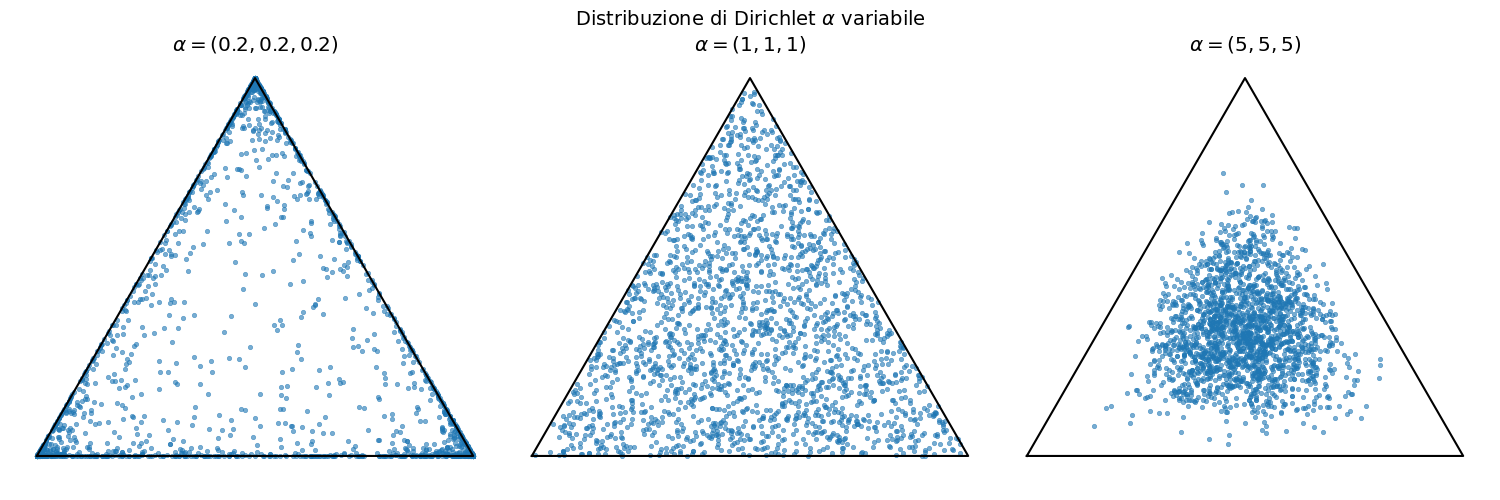
\includegraphics[width=\textwidth]{images/th_10_12/dirichlet.png}
    \caption{Esempio di distribuzione di Dirichlet tramite simplesso 2D. Le regioni colorate rappresentano diverse modalità della distribuzione.}
    \label{fig:dirichlet}
\end{figure}

\begin{proposizione}{Valore Atteso}{dirichlet-valore-atteso}
Il valore atteso di un vettore $X \sim \text{Dirichlet}(\alpha)$ è:
$$
E[X_i] = \frac{\alpha_i}{\sum_{j=1}^{m} \alpha_j} \implies E[X] = \frac{1}{S}
\alpha
$$
dove $S = \sum_{j=1}^{m} \alpha_j$.
\end{proposizione}

\begin{nota}{Relazione con la distribuzione Beta}{dirichlet-beta}
Per $m=2$, la distribuzione di Dirichlet è equivalente alla distribuzione Beta.
$$
\text{Dirichlet}(\alpha_1, \alpha_2) \equiv \text{Beta}(\alpha_1, \alpha_2)
$$
Inoltre, se $X_1 \sim \text{Unif}(0,1)$ (che è una $\text{Beta}(1,1)$) e $X_2 =
1 - X_1$, allora il vettore $(X_1, X_2) \sim \text{Dirichlet}(1, 1)$.
\end{nota}

I parametri $\alpha_i$ controllano la forma della distribuzione. Valori di
$\alpha_i < 1$ spingono la massa di probabilità verso i vertici del simplesso.
Valori di $\alpha_i > 1$ spingono la massa verso il centro. Se tutti gli
$\alpha_i$ sono uguali, la distribuzione è simmetrica. Se sono diversi, la
distribuzione è sbilanciata verso il vertice corrispondente all' $\alpha_i$
più grande.

\include{lectures/th_13-15}
\subsection{Mean Squared Error Loss (MSE)}\label{subsec:mse}

La \textbf{Mean Squared Error Loss (MSE)} è una funzione di perdita ampiamente utilizzata per i modelli di regressione, particolarmente quando i dati sono distribuiti secondo una \textbf{distribuzione gaussiana}. Essa misura la media dei quadrati delle differenze tra i valori osservati e quelli predetti dal modello.

\begin{definizione}{MSE}{mse}
La \textbf{MSE} per \( n \) osservazioni è definita come:
\[
\mathrm{MSE} = \frac{1}{n} \sum_{i=1}^n \left( y_i - \hat{y}_i \right)^2
\]
dove \( y_i \) è il valore osservato e \( \hat{y}_i \) è il valore predetto dal modello.
\end{definizione}

\subsubsection*{Distribuzione dei dati}

Nel contesto dei dati Gaussiani, supponiamo che \( Y(i) \) sia distribuito come \( Y(i) \sim \mathcal{N}(\mu(i), \sigma^2(i)) \), con \( \mu(i) \) e \( \sigma(i) \) dipendenti dal parametro \( x(i) \).

La funzione di verosimiglianza per \( n \) osservazioni è quindi:

\[
\ell(\mu(i), \sigma(i)) = \sum_{i=1}^n \left[-\log(\sqrt{2\pi}) -\log(\sigma(i)) - \frac{(y(i) - \mu(i))^2}{2\sigma(i)^2} \right]
\]
Dove:
\begin{itemize}
    \item \( \mu(i) \) è la media prevista,
    \item \( \sigma(i) \) è la deviazione standard prevista per il dato \( i \).
\end{itemize}

\subsubsection{I casi}

\begin{itemize}
    \item \textbf{Caso 1: Nessuna dipendenza dall'input (\Cref{ex:mle-norm})}: Se non c'è dipendenza da \( x(i) \), la funzione di log-verosimiglianza diventa:
        \[
            \ell(\mu, \sigma) = C - n \log \sigma - \frac{1}{2\sigma^2} \sum_{i=1}^n (y(i) - \mu)^2
        \]
        Risolvendo, otteniamo lo stimatore per la media e la deviazione standard:
        \[
            \hat{\mu} = \frac{1}{n} \sum_{i=1}^n y(i), \quad \hat{\sigma}^2 = \frac{1}{n} \sum_{i=1}^n (y(i) - \hat{\mu})^2
        \]

    \item \textbf{Caso 2: Modello regressivo con varianza costante (\textit{omoschedastico})}: Se la deviazione standard \( \sigma(i) \) è costante, e i parametri \( \mu(i) \) dipendono da \( x(i) \), possiamo assumere una relazione parametrica. Ad esempio, un modello lineare potrebbe essere usato per descrivere:
        \[
            \sigma(i) = \sigma, \quad \mu(i) = \nu(x(i); \vec{\alpha})
        \]
        La funzione di log-verosimiglianza diventa:
        \[
            \ell(\sigma, \vec{\alpha}) = C - n \log \sigma - \frac{1}{2\sigma^2} \sum_{i=1}^n (y(i) - \nu(x(i); \vec{\alpha}))^2
        \]
        Introduciamo la funzione \textbf{SE} (\textit{Squared Error}) che calcola la differenza al quadrato degli argomenti:
        \[
            \mathrm{SE}(y, z) = (y - z)^2
        \]
        Questo permette di riscrivere la log-verosimiglianza in funzione della
        MSE (\Cref{def:mse}):
        \[
            \mathrm{loss}_{\text{MSE}}(\vec{\alpha}) = \frac{1}{n} \sum_{i=1}^n \mathrm{SE}(y(i), \nu(x(i); \vec{\alpha})) = \frac{1}{n} \sum_{i=1}^n (y(i) - \nu(x(i); \vec{\alpha}))^2
        \]
        \[
            \Rightarrow \ell(\sigma, \vec{\alpha}) = C - n \log \sigma - \frac{1}{2\sigma^2}
            n\,\mathrm{loss}_{\text{MSE}}(\vec{\alpha})
            = C - n (\log \sigma + \frac{1}{2\sigma^2}
            \mathrm{loss}_{\text{MSE}}(\vec{\alpha}))
        \]
        Da qui si ottiene lo stimatore \( \hat{\sigma} \):
        \[
            \hat{\sigma} = \sqrt{\mathrm{loss}_{\text{MSE}}(\vec{\alpha})}
        \]
        L'ottimizzazione degli altri parametri segue dalla minimizzazione della
        \( \mathrm{loss}_{\text{MSE}} \).

        \begin{nota}{$\mathrm{loss_{MSE}}$}{}
            La funzione $\mathrm{loss_{MSE}}$ è semplicemente definita come lo
            \textbf{scarto quadratico medio} tra i valori osservati e quelli
            predetti dal modello.
        \end{nota}

    \item \textbf{Caso 3: Dipendenza da \( x \)}: Se i parametri \( \mu(i) \) e \( \sigma(i) \) dipendono da \( x(i) \), possiamo definire la funzione di regressione come segue:
        \[
            \mu(i) = \nu(x(i); \vec{\alpha}), \quad \sigma(i) = \tau(x(i); \vec{\alpha})
        \]
        Dove \( \nu(x(i); \vec{\alpha}) \) è il modello di regressione e \( \tau(x(i); \vec{\alpha}) \) è la variabilità associata.

        \begin{nota}{Stima di $\vec{\alpha}$}{}
            Questa funzione viene ottimizzata usando metodi iterativi, come la discesa
            del gradiente, per trovare i migliori parametri.
        \end{nota}
\end{itemize}



\section{Regressione Lineare Semplice}\label{sec:regressione}

La \textbf{regressione lineare semplice} è uno dei modelli più basilari in statistica e machine learning. In questo caso, si cerca di modellare la relazione tra una variabile dipendente \( Y \) e una variabile indipendente \( X \).

\subsection{Modello e parametri}

Il modello della regressione lineare semplice assume che la variabile dipendente \( Y \) sia una combinazione lineare della variabile indipendente \( X \), più un errore \( \epsilon \). In altre parole:
\[
Y_i = \beta_0 + \beta_1 X_i + \epsilon_i
\]
dove:
\begin{itemize}
\item \( Y_i \) è la variabile dipendente (osservazione), che si assume essere normalmente distribuita: 
    \[ Y_i \sim \mathcal{N}(\beta_0 + \beta_1 X_i, \sigma^2), \]
\item \( X_i \) è la variabile indipendente, che viene trattata come una variabile deterministica (osservata),
\item \( \beta_0 \) è l'intercetta del modello,
\item \( \beta_1 \) è la pendenza della retta di regressione,
\item \( \epsilon_i \) è l'errore, che si assume essere normalmente distribuito con media zero e varianza costante \( \sigma^2 \):
        \[ \epsilon_i \sim \mathcal{N}(0, \sigma^2). \]
\end{itemize}

Il modello descrive una \textbf{retta di regressione} che approssima la relazione tra \( X \) e \( Y \).

\begin{definizione}{Parametri del modello}{regressione-lineare-parametri}
I parametri del modello di regressione lineare sono \( \beta_0 \) (intercetta), \( \beta_1 \) (pendenza), e \( \sigma^2 \) (varianza dell'errore).
\end{definizione}

\begin{nota}{Assunzioni del modello}{reg-lin-assunzioni}
Il modello di regressione lineare semplice assume che:
\begin{itemize}
    \item La relazione tra \( X \) e \( Y \) sia lineare.
    \item Gli errori \( \epsilon_i \) siano indipendenti e normalmente distribuiti con media zero e varianza costante (\( \sigma^2 \)).
    \item La variabile dipendente \( Y \) segue una distribuzione normale con media \( \mu = \beta_0 + \beta_1 X_i \) e varianza costante \( \sigma^2 \): \( Y_i \sim \mathcal{N}(\beta_0 + \beta_1 X_i, \sigma^2) \).
    \item La variabile indipendente \( X \) è deterministica, mentre la variabile dipendente \( Y \) è casuale.
\end{itemize}
\end{nota}

\begin{nota}{Baricentro della regressione}{regressione-baricentro}
Il \textbf{baricentro} della regressione è il punto medio dei dati osservati, dato dalla media di \( X \) e \( Y \). In termini matematici, il baricentro \( (\overline{x}, \overline{y}) \) è dato da:
\[
\overline{x} = \frac{1}{n} \sum_{i=1}^n x_i, \quad \overline{y} = \frac{1}{n} \sum_{i=1}^n y_i
\]
\end{nota}

\subsection{Stima dei parametri tramite Maximum Likelihood (MLE)}

I parametri \( \beta_0 \), \( \beta_1 \), e \( \sigma^2 \) possono essere stimati utilizzando il metodo della massima verosimiglianza (MLE). La funzione di log-verosimiglianza è:

\[
\ell(\beta_0, \beta_1, \sigma) = C - n \log \sigma - \frac{1}{2\sigma^2} \sum_{i=1}^n (y_i - \beta_0 - \beta_1 x_i)^2
\]

Per trovare i parametri che massimizzano la log-verosimiglianza, possiamo derivare rispetto ai parametri e risolvere il sistema di equazioni. I parametri stimati risultano:

\begin{definizione}[
    enhanced,
    overlay last={
        \node[anchor=south east, font=\large, text=cs@definition] at (frame.south east) {$\bigstar$};
    }
]{Stima della pendenza}{regressione-lineare-pendenza}
    Lo stimatore per la pendenza \( \hat{\beta}_1 \) nel modello di regressione lineare è dato dalla seguente espressione:
    \[
        \hat{\beta}_1 = \frac{\overline{xy} - \overline{x}\, \overline{y}}{\overline{x^2} - \overline{x}^2}
    \]
    dove:
    \begin{itemize}
        \item \( \overline{x} = \frac{1}{n} \sum_{i=1}^n x_i \) è la media dei valori di \( x \),
        \item \( \overline{y} = \frac{1}{n} \sum_{i=1}^n y_i \) è la media dei valori di \( y \),
        \item \( \overline{xy} = \frac{1}{n} \sum_{i=1}^n x_i y_i \) è la media dei prodotti \( x_i y_i \),
        \item \( \overline{x^{2}} = \frac{1}{n} \sum_{i=1}^n x_i^2 \) è la media dei quadrati dei valori di \( x \).
    \end{itemize}
\end{definizione}
Questa formula fornisce la stima ottimale della pendenza \( \hat{\beta}_1 \) nel
caso di regressione lineare semplice.

\begin{definizione}[
    enhanced,
    overlay last={
        \node[anchor=south east, font=\large, text=cs@definition] at (frame.south east) {$\bigstar$};
    }
]{Stima dell'intercetta}{regressione-lineare-intercetta}
    La stima per l'intercetta \( \hat{\beta}_0 \) è data dalla formula:
    \[
        \hat{\beta}_0 = \overline{y} - \hat{\beta}_1 \overline{x}
    \]
    Dove:
    \begin{itemize}
        \item \( \overline{x} \) è la media dei valori di \( X \),
        \item \( \overline{y} \) è la media dei valori di \( Y \),
        \item \( \hat{\beta}_1 \) è la pendenza della retta di regressione.
    \end{itemize}
\end{definizione}

La retta di regressione \( \hat{y} = \hat{\beta}_0 + \hat{\beta}_1 x \) è costruita in modo che minimizzi la somma dei quadrati degli errori tra i valori osservati e quelli predetti. Un risultato interessante della regressione lineare è che questa retta passa sempre per il \textbf{baricentro} il  dei dati, dato dalle medie \( \overline{x} \) e \( \overline{y} \).

\begin{dimostrazione}{Baricentro appartiene alla regressione lineare}{}
Per \( x = \overline{x} \), la retta di regressione assume il valore:
\[
\hat{y}(\overline{x}) = \hat{\beta}_0 + \hat{\beta}_1 \overline{x}
\]
Sostituendo \( \hat{\beta}_0 = \overline{y} - \hat{\beta}_1 \overline{x} \) nella formula della retta otteniamo:
\[
\hat{y}(\overline{x}) = \left( \overline{y} - \hat{\beta}_1 \overline{x} \right) + \hat{\beta}_1 \overline{x} = \overline{y}
\]
\end{dimostrazione}

\begin{dimostrazione}{Calcolo degli stimatori \( \beta_0 \) e \( \beta_1 \)}{calcolo-b1-b0}

Partiamo dalla funzione di perdita MSE, che nel caso della regressione lineare è definita come:
\[
\text{loss}_{\text{MSE}} (\hat{\beta_0}, \hat{\beta_1}) = \frac{1}{n} \sum_{i=1}^n \left( y_i - \hat{y}_i \right)^2
\]
dove \( \hat{y}_i = \hat{\beta_0} + \hat{\beta_1} x_i \) sono i valori predetti dal modello, \( y_i \) sono i valori osservati, e \( x_i \) sono i valori delle variabili indipendenti.

Espandendo questa espressione otteniamo:
\[
\text{loss}_{\text{MSE}} (\hat{\beta_0}, \hat{\beta_1}) = \frac{1}{n} \sum_{i=1}^n \left( y_i - \hat{\beta_0} - \hat{\beta_1} x_i \right)^2
\]

Ora, per trovare i parametri \( \hat{\beta_0} \) e \( \hat{\beta_1} \), dobbiamo minimizzare questa funzione di perdita rispetto a \( \hat{\beta_0} \) e \( \hat{\beta_1} \). Questo può essere fatto derivando la funzione rispetto a ciascun parametro e ponendo le derivate uguali a zero.

Cominciamo derivando la funzione di perdita rispetto a \( \hat{\beta_0} \):

\[
    \frac{\partial \text{loss}_{\text{MSE}}}{\partial \hat{\beta_0}} = \frac{2}{n} \sum_{i=1}^n \left( y_i - \hat{\beta_0} - \hat{\beta_1} x_i \right) (-1)
\]
Poniamo questa derivata uguale a zero:
\begin{align*}
    0 &= \frac{2}{n} \sum_{i=1}^n \left( y_i - \hat{\beta_0} - \hat{\beta_1} x_i \right)\\
    \Leftrightarrow \sum_{i=1}^n y_i &= n \hat{\beta_0} + \hat{\beta_1} \sum_{i=1}^n x_i
\end{align*}
Poiché \( \sum_{i=1}^n x_i = n \overline{x} \) e \( \sum_{i=1}^n y_i = n \overline{y} \), otteniamo:
\begin{align*}
    n \overline{y} &= n \hat{\beta_0} + \hat{\beta_1} n \overline{x}\\
    \Leftrightarrow \hat{\beta_0} &= \overline{y} - \hat{\beta_1} \overline{x}
\end{align*}

Adesso deriviamo la funzione di perdita rispetto a \( \hat{\beta_1} \):

\[
    \frac{\partial \text{loss}_{\text{MSE}}}{\partial \hat{\beta_1}} = \frac{2}{n} \sum_{i=1}^n \left( y_i - \hat{\beta_0} - \hat{\beta_1} x_i \right) (-x_i)
\]
Poniamo anche questa derivata uguale a zero:
\begin{align*}
    0 &= \frac{2}{n} \sum_{i=1}^n \left( y_i - \hat{\beta_0} - \hat{\beta_1} x_i \right) (-x_i)\\
    \Rightarrow \sum_{i=1}^n x_i y_i &= \hat{\beta_0} \sum_{i=1}^n x_i + \hat{\beta_1} \sum_{i=1}^n x_i^2
\end{align*}
Sostituendo \( \hat{\beta_0} = \overline{y} - \hat{\beta_1} \overline{x} \), otteniamo:
\begin{align*}
    \sum_{i=1}^n x_i y_i &= \left( \overline{y} - \hat{\beta_1} \overline{x} \right) \sum_{i=1}^n x_i + \hat{\beta_1} \sum_{i=1}^n x_i^2 \\
    \sum_{i=1}^n x_i y_i &= \overline{y} \sum_{i=1}^n x_i - \hat{\beta_1} \overline{x} \sum_{i=1}^n x_i + \hat{\beta_1} \sum_{i=1}^n x_i^2
\end{align*}
Poiché \( \sum_{i=1}^n x_i = n \overline{x} \), otteniamo:
\[
\sum_{i=1}^n x_i y_i = n \overline{y} \overline{x} - n \hat{\beta_1} \overline{x}^2 + \hat{\beta_1} \sum_{i=1}^n x_i^2
\]
Ora, raccogliamo i termini con \( \hat{\beta_1} \):
\[
\hat{\beta_1} = \frac{\sum_{i=1}^n x_i y_i - n \overline{y} \overline{x}}{\sum_{i=1}^n x_i^2 - n \overline{x}^2}
\]
Questa è la formula per \( \hat{\beta_1} \).

Ora possiamo sostituire \( \hat{\beta_1} \) nella formula per \( \hat{\beta_0} \):
\[
\hat{\beta_0} = \overline{y} - \hat{\beta_1} \overline{x}
\]

In questo modo, abbiamo calcolato gli stimatori \( \hat{\beta_0} \) e \( \hat{\beta_1} \) utilizzando la minimizzazione della funzione di perdita MSE.

\end{dimostrazione}


\subsection{Errore Standard del modello}

L'errore standard \( S_e \) della stima del modello di regressione è definito come:

\[
S_e = \sqrt{\frac{1}{n-2} \sum_{i=1}^n (y_i - \hat{y}_i)^2}
\]
dove \( \hat{y}_i = \hat{\beta_0} + \hat{\beta_1} x_i \) è il valore predetto dalla retta di regressione.



\section{Teorema di Cochran}

\subsection{Teorema per il ML}
\begin{teorema}{Versione ML del Teorema di Cochran}{cochran-ml}
Supponiamo di essere nel caso MSE loss omoschedastico:
\[
Y(i) \sim \mathcal{N}(\mu(i), \sigma^2)
\]
con $\sigma \equiv \sigma(i)$ costante. Supponiamo inoltre:
\[
    \mu(i) = \gamma_1 c_1(x(i)) + \dots + \gamma_k c_k(x(i)) = \gamma \cdot c(x(i)), \quad \gamma,c \in \mathbb{R}^k
\]
cioè una combinazione lineare dei valori $c_1(x(i)), \ldots, c_k(x(i))$ con i parametri $\gamma_1, \ldots,
\gamma_k$.

Gli stimatori MLE dei parametri si trovano minimizzando la loss:
\[
\operatorname{loss}_{\text{MSE}}(\gamma_1, \dots, \gamma_k) = \frac{1}{n} \sum_{i=1}^n (Y(i) - \gamma \cdot c(x(i)))^2
\]
equivalente a minimizzare:
\[
    W(\gamma) = \| Y - C(x) \cdot \gamma \|^2 \qquad \text{(norma quadra del vettore
    differenza)}
\]
dove $C(x)$ è una matrice in $\mathbb{R}^{n \times k}$ le cui colonne sono date dai vettori:
\[
\begin{bmatrix}
c_j(x(i)) \\
\vdots \\
c_j(x(i))
\end{bmatrix}, \quad i = 1, \dots, n,\, j = 1, \dots, k
\]
Al variare di $\gamma$, l'immagine $\gamma \cdot C(x)$ è un sottospazio vettoriale di dimensione $k$ in $\mathbb{R}^n$. Lo stimatore $\hat{\gamma}$ è la proiezione ortogonale di $Y$ su questo sottospazio.

Si definisce la somma dei quadrati dei residui come:
\[
    SSR = W(\hat{\gamma})
\]
Allora:
\begin{enumerate}
    \item $\hat{\gamma}$ è uno stimatore corretto di $\gamma$ e la sua formula è:
        \begin{equation*}\label{eq:cochran-gamma-estimator}
            \hat{\gamma} = (C^T C)^{-1} C^T Y
        \end{equation*}
    \item \( \frac{SSR}{\sigma^2} \sim \chi^2(n-k) \), quindi \( \frac{SSR}{n-k} \) è uno stimatore corretto di $\sigma^2$;
  \item $\hat{\gamma}$ e $SSR$ sono variabili aleatorie indipendenti.
\end{enumerate}
\end{teorema}

\begin{dimostrazione}{Formula per la proiezione}{projection-formula}
Dato che il modello è lineare, esiste una formula esplicita per calcolare la proiezione ortogonale $\hat{\gamma}$ di $Y$ sul sottospazio generato dalle colonne della matrice $C$.
La formula è:
\[
\hat{\gamma} = (C^T C)^{-1} C^T Y
\]
Per verificarla, minimizziamo la funzione di costo $W(\gamma)$ calcolandone le derivate parziali rispetto a ciascun parametro $\gamma_j$ e ponendole a zero.
\[
W(\gamma) = \| Y - C\gamma \|^2 = \sum_{i=1}^{n} \left(Y_i - (C\gamma)_i\right)^2 = \sum_{i=1}^{n} \left(Y_i - \sum_{j=1}^{k} C_{ij}\gamma_j\right)^2
\]
Calcoliamo la derivata parziale rispetto a $\gamma_h$:
\[
\frac{\partial W(\gamma)}{\partial \gamma_h} = \sum_{i=1}^{n} 2 \left(Y_i - \sum_{j=1}^{k} C_{ij}\gamma_j\right) (-C_{ih}) = 0
\]
Questo implica:
\[
\sum_{i=1}^{n} \sum_{j=1}^{k} C_{ij} C_{ih} \hat{\gamma}_j = \sum_{i=1}^{n} Y_i C_{ih} \quad \forall h=1, \dots, k
\]
Riscrivendo l'equazione in forma matriciale:
\[
(C^T C \hat{\gamma})_h = \sum_{i,j} C^T_{hi} C_{ij} \hat{\gamma}_j = \sum_{i} C^T_{hi} Y_i = (C^T Y)_h
\]
Otteniamo quindi:
\[
C^T C \hat{\gamma} = C^T Y \implies \hat{\gamma} = (C^T C)^{-1} C^T Y
\]
\end{dimostrazione}

\subsection{Teorema per le applicazioni}
\begin{teorema}{Versione applicativa del Teorema di Cochran}{cochran-app}
Siano $X_1, \dots, X_n$ variabili aleatorie indipendenti con
\[
X_i \sim \mathcal{N}(\mu_i, \sigma^2)
\]
(modello omoschedastico). Supponiamo inoltre che
\[
\mu = (\mu_1, \dots, \mu_n)^T \in V \subseteq \mathbb{R}^n
\]
dove $V$ è un sottospazio vettoriale di dimensione $k$ assegnato.

Allora valgono i seguenti risultati:
\begin{enumerate}
  \item Lo stimatore ML di $\mu$ è la proiezione ortogonale
        $\pi_V(X)$ di $X$ su $V$;
  \item $\pi_V(X)$ è uno stimatore corretto di $\mu$;
  \item La quantità
        \[
        W := \| X - \pi_V(X) \|^2
        \]
        è indipendente da $\pi_V(X)$ e
        \[
        \frac{W}{\sigma^2} \sim \chi^2(n - k).
        \]
\end{enumerate}
\end{teorema}

\begin{esempio}{Proiezione ortogonale in $\mathbb{R}^3$}{cochran-esempio-ml}
Sia $Y \in \mathbb{R}^3$ un vettore aleatorio e sia $C\hat{\gamma}$ un sottospazio
piano (di dimensione $k=2$). Il punto $\hat{Y} = C\hat{\gamma}$ rappresenta la
proiezione ortogonale di $Y$ sul piano generato da $C$.

Definiamo la somma dei quadrati dei residui come:
\[
SSR = \| Y - C\hat{\gamma} \|^2
\]

Il teorema di Cochran assicura che:
\begin{itemize}
  \item $\hat{\gamma}$ è uno stimatore corretto di $\gamma$;
  \item $\hat{\gamma}$ è indipendente da $SSR$;
  \item $\frac{SSR}{\sigma^2} \sim \chi^2(n-k)$.
\end{itemize}
\end{esempio}

\begin{esempio}{Campione Gaussiano e t-Student}{gaussian-example}
Consideriamo un campione i.i.d. $Y_1, \dots, Y_n \sim \mathcal{N}(\mu, \sigma^2)$. In questo caso, il modello di media è $\mu(i) = \mu = \gamma_1 \cdot 1$, quindi $k=1$ e il regressore è $c_1(x(i))=1$ per ogni $i$.
La matrice $C$ è un vettore colonna di $n$ uni:
\[
C = \begin{pmatrix} 1 \\ \vdots \\ 1 \end{pmatrix}
\]
Calcoliamo le matrici necessarie per la proiezione:
\[
C^T C = \begin{pmatrix} 1 & \dots & 1 \end{pmatrix} \begin{pmatrix} 1 \\ \vdots \\ 1 \end{pmatrix} = n
\]
\[
C^T Y = \begin{pmatrix} 1 & \dots & 1 \end{pmatrix} \begin{pmatrix} Y_1 \\ \vdots \\ Y_n \end{pmatrix} = \sum_{i=1}^n Y_i
\]
Lo stimatore di massima verosimiglianza per $\mu$ è quindi la media campionaria:
\[
\hat{\mu} = \hat{\gamma}_1 = (C^T C)^{-1} C^T Y = \frac{1}{n} \sum_{i=1}^n Y_i = \bar{Y}
\]
La somma dei quadrati dei residui (SSR) è:
\[
SSR = \sum_{i=1}^n (Y_i - \mu(i))^2 = \sum_{i=1}^n (Y_i - \bar{Y})^2
\]
Definiamo la varianza campionaria corretta $S_X^2$ come:
\[
S_X^2 = \frac{1}{n-1} \sum_{i=1}^n (Y_i - \bar{Y})^2 = \frac{SSR}{n-1}
\]
Per il teorema di Cochran, sappiamo che $\bar{Y}$ e $S_X^2$ sono indipendenti e che $\frac{SSR}{\sigma^2} = \frac{(n-1)S_X^2}{\sigma^2} \sim \chi^2(n-1)$.

Sfruttando questi risultati, possiamo costruire una statistica t-Student. Ricordiamo la definizione operativa:
\begin{nota}{t-Student}{}
Siano $Z \sim \mathcal{N}(0,1)$ e $W \sim \chi^2(k)$ due variabili aleatorie indipendenti. Allora la variabile
\[
T = \frac{Z}{\sqrt{W/k}}
\]
segue una distribuzione t-Student con $k$ gradi di libertà, denotata con $t(k)$.
\end{nota}
Nel nostro caso, la media campionaria standardizzata è $Z$:
\[
\bar{Y} \sim \mathcal{N}\left(\mu, \frac{\sigma^2}{n}\right) \implies Z = \frac{\bar{Y} - \mu}{\sigma/\sqrt{n}} \sim \mathcal{N}(0,1)
\]
e la variabile $W$ è $\frac{(n-1)S_X^2}{\sigma^2}$. Sostituendo nella formula della t-Student otteniamo:
\[
\frac{\frac{\bar{Y}-\mu}{\sigma/\sqrt{n}}}{\sqrt{\frac{(n-1)S_X^2/\sigma^2}{n-1}}} = \frac{\frac{\bar{Y}-\mu}{\sigma/\sqrt{n}}}{\sqrt{\frac{S_X^2}{\sigma^2}}} = \frac{\bar{Y}-\mu}{S_X/\sqrt{n}} \sim t(n-1)
\]
Questa statistica è fondamentale per costruire intervalli di confidenza e test di ipotesi sulla media $\mu$ quando la varianza $\sigma^2$ non è nota.
\end{esempio}

\begin{proposizione}{Distribuzione dello stimatore $\hat{\gamma}$}{gamma-dist}
Nelle ipotesi del modello di regressione lineare (\Cref{thm:cochran-ml}), lo stimatore di massima verosimiglianza $\hat{\gamma}$ segue una distribuzione Normale multivariata. È uno stimatore corretto, con valore atteso $\gamma$, e la sua matrice di covarianza è $\sigma^2(C^TC)^{-1}$.
In sintesi:
\[
\hat{\gamma} \sim \mathcal{N}(\gamma, \sigma^2 (C^T C)^{-1})
\]
\end{proposizione}

\begin{dimostrazione}{}{gamma-dist}
Lo stimatore $\hat{\gamma}$ è una trasformazione lineare del vettore aleatorio Gaussiano $Y \in \mathbb{R}^n$.
\[
\hat{\gamma} = \underbrace{(C^T C)^{-1} C^T}_{N} Y
\]
dove $N$ è una matrice deterministica $k \times n$.
Dato che $Y(i) \sim \mathcal{N}(\mu(i), \sigma^2)$ sono indipendenti, il vettore $Y$ ha distribuzione $Y \sim \mathcal{N}(\mu, \sigma^2 I_n)$, dove per ipotesi $\mu = C\gamma$.

Una trasformazione lineare di un vettore Gaussiano è ancora Gaussiana. Per definirla, ne calcoliamo valore atteso e matrice di covarianza.

\textbf{Valore atteso (Correttezza):}
\[
E[\hat{\gamma}] = E[NY] = NE[Y] = N\mu = (C^T C)^{-1} C^T (C\gamma) = (C^T C)^{-1} (C^T C) \gamma = \gamma
\]
Lo stimatore $\hat{\gamma}$ è quindi corretto (unbiased).

\textbf{Matrice di Covarianza:}
\begin{align*}
\text{Cov}(\hat{\gamma}) &= \text{Cov}(NY) = N \text{Cov}(Y) N^T = N (\sigma^2 I_n) N^T = \sigma^2 NN^T \\
&= \sigma^2 \left((C^T C)^{-1} C^T\right) \left((C^T C)^{-1} C^T\right)^T \\
&= \sigma^2 (C^T C)^{-1} C^T C ((C^T C)^{-1})^T
\end{align*}
Poiché $(C^T C)$ è simmetrica, anche la sua inversa lo è, quindi $((C^T C)^{-1})^T = (C^T C)^{-1}$.
\[
\text{Cov}(\hat{\gamma}) = \sigma^2 (C^T C)^{-1} (C^T C) (C^T C)^{-1} = \sigma^2 (C^T C)^{-1}
\]
Avendo determinato media e covarianza, la distribuzione è completamente specificata.
\end{dimostrazione}


\subsection{Applicazione: Regressione Lineare Semplice}

\begin{esempio}{Regressione Lineare Semplice}{simple-regression}
Consideriamo il modello di regressione lineare semplice:
\[
Y(i) \sim \mathcal{N}(\mu(i), \sigma^2) \quad \text{con} \quad \mu(i) = \beta_0 + \beta_1 x(i)
\]
Questo è un modello lineare con $k=2$ parametri, $\gamma = (\beta_0, \beta_1)^T$. Le funzioni base sono $c_1(x)=1$ e $c_2(x)=x$. La matrice dei regressori $C$ è:
\[
C = \begin{pmatrix}
1 & x(1) \\
1 & x(2) \\
\vdots & \vdots \\
1 & x(n)
\end{pmatrix}
\]
Calcoliamo $C^T C$:
\[
C^T C = \begin{pmatrix}
\sum 1 & \sum x(i) \\
\sum x(i) & \sum x(i)^2
\end{pmatrix} = n \begin{pmatrix}
1 & \bar{x} \\
\bar{x} & \overline{x^2}
\end{pmatrix}
\]
La sua inversa è:
\[
(C^T C)^{-1} = \frac{1}{n(\overline{x^2} - \bar{x}^2)} \begin{pmatrix}
\overline{x^2} & -\bar{x} \\
-\bar{x} & 1
\end{pmatrix}
\]
Applicando la \Cref{prop:gamma-dist}, la distribuzione del vettore degli stimatori $\hat{\gamma} = (\hat{\beta}_0, \hat{\beta}_1)^T$ è:
\[
\begin{pmatrix} \hat{\beta}_0 \\ \hat{\beta}_1 \end{pmatrix} \sim \mathcal{N} \left( \begin{pmatrix} \beta_0 \\ \beta_1 \end{pmatrix}, \frac{\sigma^2}{n(\overline{x^2}-\bar{x}^2)} \begin{pmatrix} \overline{x^2} & -\bar{x} \\ -\bar{x} & 1 \end{pmatrix} \right)
\]
Grazie a una proprietà fondamentale della distribuzione Normale multivariata, possiamo ricavare immediatamente le distribuzioni dei singoli stimatori (le \textbf{distribuzioni marginali}). La media di ogni stimatore è l'elemento corrispondente nel vettore delle medie, e la sua varianza è l'elemento corrispondente sulla diagonale principale della matrice di covarianza.
\begin{itemize}
    \item Per $\hat{\beta}_0$, prendiamo il primo elemento della media ($\beta_0$) e il primo elemento sulla diagonale della matrice di covarianza:
    \[
    \hat{\beta}_0 \sim \mathcal{N}\left(\beta_0, \frac{\sigma^2\overline{x^2}}{n(\overline{x^2}-\bar{x}^2)}\right)
    \]
    \item Per $\hat{\beta}_1$, prendiamo il secondo elemento della media ($\beta_1$) e il secondo elemento sulla diagonale:
    \[
    \hat{\beta}_1 \sim \mathcal{N}\left(\beta_1, \frac{\sigma^2}{n(\overline{x^2}-\bar{x}^2)}\right)
    \]
\end{itemize}
La somma dei quadrati dei residui è $SSR = \sum(Y(i) - (\hat{\beta}_0 +
\hat{\beta}_1 x(i)))^2$. Lo stimatore non distorto della varianza $\sigma^2$ è
$S_e^2 = \frac{SSR}{n-2}$\label{eq:se-lin-regr}. Per il Teorema di Cochran, $\frac{SSR}{\sigma^2} \sim
\chi^2(n-2)$ ed è indipendente da $\hat{\gamma}$.
\end{esempio}

% ===================================================================
% SEZIONE 1: RICHIAMI DI INFERENZA STATISTICA
% ===================================================================
\section{Richiami di Inferenza Statistica: Il Test d'Ipotesi}

L'inferenza statistica fornisce gli strumenti per trarre conclusioni su una
popolazione partendo da dati campionari, che sono intrinsecamente affetti da
variabilità casuale. Il test di ipotesi è la procedura formale per prendere
decisioni in condizioni di incertezza.

\begin{nota}{Analogia: Il Tribunale della Statistica}{courtroom-analogy}
	Un test di ipotesi funziona come un processo in tribunale:
	\begin{itemize}
		\item L'\textbf{ipotesi nulla ($H_0$)} è l'imputato, presunto innocente
		      (status quo).
		\item I \textbf{dati campionari} sono le prove presentate.
		\item Lo \textbf{statistico} è il giudice che valuta se le prove sono
		      abbastanza schiaccianti da rifiutare l'ipotesi nulla.
	\end{itemize}
\end{nota}

\subsection{Le Componenti Fondamentali di un Test}

\begin{definizione}{Ipotesi Nulla ($H_0$) e Alternativa ($H_1$)}{hypotheses-def}
	Ogni test si fonda su due ipotesi contrapposte e mutualmente esclusive:
	\begin{itemize}
		\item \textbf{Ipotesi Nulla ($H_0$)}: L'ipotesi dell'assenza di un
		      effetto. Afferma che ogni differenza osservata è dovuta al caso. È
		      l'ipotesi che cerchiamo di smentire (es. $H_0: \mu = 100$).
		\item \textbf{Ipotesi Alternativa ($H_1$)}: L'ipotesi che si contrappone
		      alla nulla. Può essere \textbf{bilaterale} (es. $H_1: \mu \neq 100$) o
		      \textbf{unilaterale} (es. $H_1: \mu > 100$).
	\end{itemize}
\end{definizione}

\begin{definizione}{Statistica Test e p-value}{test-stat-pvalue-def}
	\begin{itemize}
		\item \textbf{Statistica Test}: Un valore calcolato dai dati campionari
		      che misura quanto questi si discostino da ciò che ci aspetteremmo se
		      $H_0$ fosse vera.
		\item \textbf{p-value}: La probabilità di osservare un valore della
		      statistica test altrettanto o più estremo di quello ottenuto,
		      \textit{assumendo che l'ipotesi nulla sia vera}. Un p-value piccolo
		      indica che i dati osservati sono improbabili sotto $H_0$.
	\end{itemize}
\end{definizione}

\paragraph{La Regola di Decisione.} Si fissa una soglia di significatività
$\alpha$ (solitamente 0.05).
\begin{itemize}
	\item \textbf{Se p-value $<\alpha$}: Si rifiuta $H_0$. Il risultato è
	      statisticamente significativo.
	\item \textbf{Se p-value $\geq \alpha$}: Non si rifiuta $H_0$. Non abbiamo
	      prove sufficienti per smentirla.
\end{itemize}

\subsection{Errori e Potenza di un Test}

Nel prendere una decisione basata su un test di ipotesi, ci sono quattro
possibili esiti che possono essere riassunti in una tabella di contingenza,
spesso chiamata matrice di confusione del test.

\begin{center}
	\begin{tabular}{cc|c|c|}
		                & \multicolumn{1}{c}{}              &
		\multicolumn{2}{c}{\textbf{Decisione Presa}}                                              \\
		                & \multicolumn{1}{c}{}              & \multicolumn{1}{c}{Non Rifiuto
		$H_0$}          & \multicolumn{1}{c}{Rifiuto $H_0$}                                       \\
		\cline{3-4}
		\textbf{Realtà} & $H_0$ è Vera                      & \textit{Decisione Corretta}       &
		\textbf{Errore I Tipo} $(\alpha)$                                                         \\
		\cline{3-4}
		                & $H_0$ è Falsa                     & \textbf{Errore II Tipo} $(\beta)$ &
		\textit{Decisione Corretta}                                                               \\
		\cline{3-4}
	\end{tabular}
\end{center}

\begin{definizione}{Errori di I e II Tipo e Potenza}{errors-power-def}
	\begin{itemize}
		\item \textbf{Errore di I Tipo (Falso Positivo)}: Rifiutare un'$H_0$
		      vera. La sua probabilità è $\alpha$.
		\item \textbf{Errore di II Tipo (Falso Negativo)}: Non rifiutare
		      un'$H_0$ falsa. La sua probabilità è $\beta$.
		\item \textbf{Potenza del Test}: La probabilità di rifiutare
		      correttamente un'$H_0$ falsa. È definita come \textbf{Potenza $= 1 -
				      \beta$}.
	\end{itemize}
\end{definizione}


% ===================================================================
% SEZIONE 2: REGRESSIONE LINEARE E INFERENZA
% ===================================================================
\section{Inferenza nel Modello di Regressione Lineare}

Applichiamo ora i concetti di inferenza al modello di regressione lineare per
valutare la significatività dei parametri stimati.

\subsection{Regressione Lineare Semplice}

\subsubsection{\texorpdfstring{Test di Ipotesi sul Coefficiente
		\(\beta_1\)}{Test di Ipotesi sul Coefficiente beta1}}

\paragraph{Obiettivo:} Verificare se esista una relazione lineare
statisticamente significativa tra la variabile di input \(X\) e la variabile di
risposta \(Y\), rispondendo alla domanda: "Y dipende davvero da X?".

\paragraph{Ipotesi:}
Le ipotesi statistiche per il parametro \(\beta_1\) sono:
\begin{itemize}
	\item \textbf{Ipotesi Nulla $H_0$}: $\beta_1 = 0$ (non c'è relazione
	      lineare; la pendenza è nulla).
	\item \textbf{Ipotesi Alternativa $H_1$}: $\beta_1 \neq 0$ (esiste una
	      relazione lineare).
\end{itemize}

\paragraph{Procedura di Derivazione della Statistica Test:}
La costruzione della statistica test parte dalla distribuzione dello stimatore
\(B_1\) e segue una serie di passaggi di standardizzazione.

\begin{enumerate}
	\item \textbf{Distribuzione dello Stimatore:} Lo stimatore \(B_1\) segue una
	      distribuzione Normale la cui varianza è nota dalla teoria (si veda
	      l'applicazione del Teorema di Cochran).
	      \[
		      B_1 \sim \mathcal{N}\left(\beta_1,
		      \frac{\sigma^2}{n(\overline{x^2}-\bar{x}^2)}\right)
	      \]

	\item \textbf{Funzione Ancillare (Normale):} Standardizzando \(B_1\) si
	      ottiene una variabile con distribuzione \(\mathcal{N}(0,1)\), che però
	      dipende ancora dal parametro ignoto \(\sigma\).
	      \[
		      \frac{B_1 - \beta_1}{\sigma} \sqrt{n(\overline{x^2}-\bar{x}^2)}
		      \sim \mathcal{N}(0,1)
	      \]

	\item \textbf{Funzione Ancillare (t-Student):} Sostituendo \(\sigma\) con la
	      sua stima \(S_e\), la distribuzione diventa una t-Student con \(n-2\) gradi
	      di libertà.
	      \[
		      \frac{B_1 - \beta_1}{S_e} \sqrt{n(\overline{x^2}-\bar{x}^2)} \sim
		      t(n-2)
	      \]

	\item \textbf{Statistica Test Finale:} Valutando la funzione ancillare sotto
	      l'ipotesi nulla \(H_0: \beta_1 = 0\), si ottiene la statistica test finale
	      da calcolare con i dati.
	      \[
		      T = \frac{B_1}{S_e} \sqrt{n(\overline{x^2}-\bar{x}^2)}
	      \]
\end{enumerate}

\paragraph{Metodi di Decisione:}
Una volta calcolato il valore \(T_{obs}\) della statistica test, si può
procedere in due modi:

\begin{itemize}
	\item \textbf{Regione di Accettazione (R.A.):} Si confronta \(|T_{obs}|\)
	      con un valore critico \(q\). Se \(|T_{obs}| > q\), si rifiuta \(H_0\). Il
	      valore di \(q\) è il quantile della distribuzione t-Student tale che \(q =
	      F_{t(n-2)}^{-1}(1-\alpha/2)\).

	\item \textbf{p-value:} Si calcola la probabilità di osservare un valore
	      della statistica test altrettanto o più estremo di quello ottenuto,
	      assumendo \(H_0\) vera. Per un test a due code, la formula è:
	      \[
		      \text{p-value} = 2 \cdot P(T > |T_{obs}|) = 2 \cdot (1 -
		      F_{t(n-2)}(|T_{obs}|))
	      \]
	      dove \(F_{t(n-2)}\) è la funzione di ripartizione della distribuzione
	      t-Student con \(n-2\) gradi di libertà. Se il p-value è inferiore al
	      livello di significatività \(\alpha\), si rifiuta \(H_0\).
\end{itemize}

\subsubsection{Intervallo di Confidenza per la Risposta Media}

\paragraph{Obiettivo:} L'obiettivo è stimare un intervallo di valori plausibili
non per un singolo punto, ma per la \textbf{risposta media} \(E[Y|x] = \beta_0 +
\beta_1 x\), che è una funzione. Poiché la vera retta delle medie è
sconosciuta, si costruisce un "intervallo tubolare" o \textbf{banda di
	confidenza} attorno alla retta stimata (\(B_0 + B_1x\)), all'interno del quale
si ha un'elevata fiducia che si trovi la vera retta.

\begin{nota}{Stimatore vs Valore Vero}{estimator-vs-true-value}
	È importante distinguere tra:
	\begin{itemize}
		\item Il \textbf{valore incognito da stimare}: la funzione \( \beta_0 +
		      \beta_1 x \).
		\item Lo \textbf{stimatore puntuale}: la retta di regressione calcolata
		      dai dati, \( B_0 + B_1 x \).
	\end{itemize}
	Per costruire l'intervallo, si analizza la distribuzione di questo
	stimatore.
\end{nota}

\paragraph{Proprietà dello Stimatore:} Lo stimatore \(B_0 + B_1x\) è corretto
e la sua varianza dipende da \(x\), spiegando la forma a "clessidra" della banda
di confidenza.

\begin{dimostrazione}{Calcolo di Media e Varianza dello
		Stimatore}{dem:mean-var-estimator}
	Calcoliamo il valore atteso e la varianza dello stimatore \(\hat{y}(x) = B_0
	+ B_1x\).

	\textbf{Valore Atteso (Correttezza)}
	Usando la linearità del valore atteso e sapendo che gli stimatori \(B_0\) e
	\(B_1\) sono corretti (\(E[B_0]=\beta_0\), \(E[B_1]=\beta_1\)):
	\begin{align*}
		E[B_0 + B_1x] & = E[B_0] + E[B_1x]   \\
		              & = E[B_0] + xE[B_1]   \\
		              & = \beta_0 + \beta_1x
	\end{align*}
	Lo stimatore è quindi corretto.

	\textbf{Varianza}
	Usiamo la formula della varianza di una somma di variabili aleatorie:
	\begin{align*}
		\text{Var}(B_0 + B_1x) & = \text{Var}(B_0) + \text{Var}(B_1x) +
		2\text{Cov}(B_0, B_1x)                                            \\
		                       & = \text{Var}(B_0) + x^2\text{Var}(B_1) +
		2x\text{Cov}(B_0, B_1)
	\end{align*}
	Sostituendo i termini dalla matrice di covarianza dello stimatore
	\((\hat{\beta}_0, \hat{\beta}_1)\) si ottiene:
	\[
		\text{Var}(B_0 + B_1 x) = \sigma^2 \left[ \frac{1}{n} + \frac{(x -
				\bar{x})^2}{n(\overline{x^2}-\bar{x}^2)} \right]
	\]
\end{dimostrazione}

\paragraph{Formula Finale:} Sfruttando le proprietà dello stimatore e
sostituendo \(\sigma\) con la sua stima \(S_e\), si costruisce una quantità
pivotale basata sulla distribuzione t-Student. Manipolandola algebricamente, si
ottiene l'intervallo di confidenza finale:
\[
	(B_0 + B_1 x) \pm q \cdot S_e \sqrt{\frac{1}{n} + \frac{(x -
			\bar{x})^2}{n(\overline{x^2}-\bar{x}^2)}}
\]
dove \(q = F_{t(n-2)}^{-1}(1 - \alpha/2)\) è il quantile critico della
distribuzione t-Student per un livello di confidenza di \(1-\alpha\).

\paragraph{Calcolo della Varianza con Notazione Matriciale}
È possibile calcolare le varianze per tutti i punti del dataset in un'unica
operazione. Il vettore delle risposte medie stimate è \(\hat{Y} = C
\hat{\beta}\), dove \(C\) è la matrice dei regressori \(n \times 2\).

Per trovare la varianza di ogni componente di \(\hat{Y}\), si calcola prima
l'intera matrice di covarianza di \(\hat{Y}\) usando la regola di trasformazione
per vettori aleatori:
\[
	\text{Cov}(\hat{Y}) = \text{Cov}(C \hat{\beta}) = C \text{Cov}(\hat{\beta})
	C^T
\]
Sostituendo \(\text{Cov}(\hat{\beta}) = \sigma^2 (C^T C)^{-1}\), otteniamo:
\[
	\text{Cov}(\hat{Y}) = C \left( \sigma^2 (C^T C)^{-1} \right) C^T = \sigma^2
	\left( C (C^T C)^{-1} C^T \right)
\]
Il risultato è una matrice \(n \times n\), e le varianze richieste sono gli
elementi sulla sua \textbf{diagonale principale}. Il vettore delle varianze per
ogni \(\hat{y}_i\) è quindi:
\[
	\begin{pmatrix} \text{Var}(\hat{y}_1) \\ \vdots \\ \text{Var}(\hat{y}_n)
	\end{pmatrix} = \text{diag}\left( \text{Cov}(\hat{Y}) \right)
\]

\subparagraph{Dalla Diagonale all'Intervallo di Confidenza}
Una volta calcolata la matrice di covarianza delle risposte stimate,
\(\text{Cov}(\hat{Y})\), il passo finale è costruire l'intervallo per ciascuna
delle \(n\) medie stimate \(\hat{y}_i\).

Il \(i\)-esimo elemento della diagonale, \([\text{Cov}(\hat{Y})]_{ii}\),
rappresenta la varianza della \(i\)-esima risposta media stimata,
\(\text{Var}(\hat{y}_i)\). Questa varianza dipende però dal parametro ignoto
\(\sigma^2\). Per calcolare l'intervallo, dobbiamo prima stimarla, sostituendo
\(\sigma^2\) con la sua stima corretta \(S_e^2\).

Lo \textbf{standard error} per la \(i\)-esima risposta media stimata,
\(SE(\hat{y}_i)\), è la radice quadrata di questa varianza stimata:
\[
	SE(\hat{y}_i) = \sqrt{S_e^2 \cdot \left[ C (C^T C)^{-1} C^T \right]_{ii}} =
	S_e \sqrt{\left[ C (C^T C)^{-1} C^T \right]_{ii}}
\]
dove \([ \cdot ]_{ii}\) indica l'\(i\)-esimo elemento diagonale della matrice.

L'intervallo di confidenza al livello \(1-\alpha\) per la risposta media al
punto \(x_i\) è infine:
\[
	y \in \hat{y} \pm q \cdot SE(\hat{y}_i)
\]
dove \(q = F_{t(n-2)}^{-1}(1-\alpha/2)\) è il quantile critico della
distribuzione t-Student. Applicando questa formula per ogni \(i=1, \dots, n\),
si ottengono i limiti superiore e inferiore che definiscono la banda di
confidenza.

\subsubsection{Intervallo di Predizione per una Osservazione Futura}

\paragraph{Obiettivo:} Per un nuovo valore di input \(\tilde{x}\), predire un
intervallo di valori plausibili in cui cadrà una \textbf{singola osservazione
	futura} \(\tilde{Y}\). L'obiettivo è creare una "banda di predizione" che
contenga, con alta probabilità, i futuri punti dati.

\paragraph{Differenza Chiave rispetto all'Intervallo di Confidenza:}
Questo intervallo è sempre più largo di quello di confidenza perché deve
tenere conto di \textbf{due fonti di incertezza}:
\begin{enumerate}
	\item L'incertezza sulla stima della retta di regressione (la variabilità
	      dello stimatore \(B_0 + B_1\tilde{x}\)).
	\item La variabilità intrinseca della singola osservazione futura
	      \(\tilde{Y}\), che fluttua casualmente attorno alla sua media vera (con
	      varianza \(\sigma^2\)).
\end{enumerate}

\begin{nota}{Larghezza dell'intervallo}{itv_oss_futura}
	Mentre l'intervallo di confidenza per la media si stringe all'aumentare dei
	dati, quello di predizione rimane sempre relativamente largo per via di
	questa seconda componente di incertezza.
\end{nota}

\paragraph{Proprietà dell'Errore di Predizione:} La costruzione dell'intervallo
si basa sull'analisi dell'errore di predizione, definito come la differenza tra
il valore futuro e la sua stima: \( \tilde{Y} - (B_0 + B_1\tilde{x}) \). Questo
errore ha media zero e la sua varianza è la somma delle varianze delle due
componenti di incertezza.

\begin{dimostrazione}{Calcolo di Media e Varianza dell'Errore di
		Predizione}{dem:pred-error-var}
	Consideriamo l'errore di predizione \( e_{pred} = \tilde{Y} - (B_0 +
	B_1\tilde{x}) \).

	\textbf{Valore Atteso}
	Il valore atteso dell'errore è zero.
	\begin{align*}
		E[e_{pred}] & = E[\tilde{Y} - (B_0 + B_1\tilde{x})]       \\
		            & = E[\tilde{Y}] - E[B_0 + B_1\tilde{x}]      \\
		            & = (\beta_0 + \beta_1\tilde{x}) - (\beta_0 +
		\beta_1\tilde{x}) = 0
	\end{align*}

	\textbf{Varianza}
	Data l'indipendenza tra l'osservazione futura \(\tilde{Y}\) e gli stimatori
	\(B_0, B_1\), la varianza della differenza è la somma delle varianze:
	\begin{align*}
		\text{Var}(e_{pred}) & = \text{Var}(\tilde{Y}) + \text{Var}(B_0 +
		B_1\tilde{x})                                                     \\
		                     & = \sigma^2 + \sigma^2 \left[ \frac{1}{n} +
			\frac{(\tilde{x} -
		\bar{x})^2}{n(\overline{x^2}-\bar{x}^2)} \right]                  \\
		                     & = \sigma^2 \left[ 1 + \frac{1}{n} +
			\frac{(\tilde{x} -
				\bar{x})^2}{n(\overline{x^2}-\bar{x}^2)} \right]
	\end{align*}
\end{dimostrazione}

\paragraph{Calcolo Matriciale della Varianza di Predizione}
In analogia con l'intervallo di confidenza, possiamo calcolare le varianze
dell'errore di predizione per tutti i punti del dataset simultaneamente. La
varianza dell'errore di predizione per una futura osservazione al punto \(x_i\)
è la somma di due componenti: la varianza del modello e la varianza della stima
della media in quel punto.
\[
	\text{Var}(e_{pred, i}) = \text{Var}(\tilde{Y}_i) + \text{Var}(\hat{y}_i) =
	\sigma^2 + \text{Var}(\hat{y}_i)
\]
Per ottenere il vettore di queste varianze per tutti gli \(n\) punti, sommiamo
la varianza intrinseca \(\sigma^2\) a ciascun elemento del vettore delle
varianze delle risposte medie stimate.

Ricordiamo che il vettore delle varianze per \(\hat{Y}\) è dato dalla diagonale
della sua matrice di covarianza:
\[
	\begin{pmatrix} \text{Var}(\hat{y}_1) \\ \vdots \\ \text{Var}(\hat{y}_n)
	\end{pmatrix} = \text{diag}\left( \sigma^2 C (C^T C)^{-1} C^T \right)
\]
Il vettore delle varianze dell'errore di predizione è quindi:
\[
	\begin{pmatrix} \text{Var}(e_{pred, 1}) \\ \vdots \\ \text{Var}(e_{pred, n})
	\end{pmatrix} =
	\sigma^2 \cdot \mathbf{1}_n + \text{diag}\left( \sigma^2 C (C^T C)^{-1} C^T
	\right)
	= \sigma^2 \left( \mathbf{1}_n + \text{diag}\left( C (C^T C)^{-1} C^T
	\right) \right)
\]
dove \(\mathbf{1}_n\) è un vettore colonna di \(n\) uni.

Lo \textbf{standard error} per la \(i\)-esima risposta futura stimata,
\(SE(\tilde{y}_i)\), è la radice quadrata di questa varianza stimata:
\[
	SE(\tilde{y}_i) = \sqrt{S_e^2 \cdot \left(1 + \left[ C (C^T C)^{-1} C^T
			\right]_{ii}\right)} = S_e \sqrt{1 + \left[ C (C^T C)^{-1} C^T \right]_{ii}}
\]
dove \([ \cdot ]_{ii}\) indica l'\(i\)-esimo elemento diagonale della matrice.
\[
	\tilde{y}_i \in \hat{y}_i \pm q \cdot SE(\tilde{y}_i)
\]
dove \(q = F_{t(n-2)}^{-1}(1-\alpha/2)\) è il quantile critico della
distribuzione t-Student. Applicando questa formula per ogni \(i=1, \dots, n\),
si ottengono i limiti superiore e inferiore che definiscono la banda di
confidenza.


\subsection{Regressione Lineare Multipla}

La regressione lineare multipla è un'estensione del modello semplice che
permette di utilizzare \(p\) variabili indipendenti (predittori) per modellare
una singola variabile dipendente \(Y\).

\subsubsection{Modello e Notazione Matriciale}

Il modello per una singola osservazione \(i\) assume che la risposta sia una
combinazione lineare dei predittori, più un termine di errore Gaussiano:
\[
	Y_i = \beta_0 + \beta_1 x_{i1} + \beta_2 x_{i2} + \dots + \beta_p x_{ip} +
	e_i, \quad \text{con } e_i \sim \mathcal{N}(0, \sigma^2)
\]

\begin{definizione}{Modello Matriciale}{multi-reg-model-def}
	Per gestire il modello in modo efficiente, si adotta la notazione
	matriciale. L'intero set di \(n\) equazioni può essere scritto come:
	\[
		Y = X\beta + e
	\]
	dove:
	\begin{itemize}
		\item \(Y \in \mathbb{R}^n\) è il vettore delle osservazioni della
		      variabile dipendente.
		\item \(X \in \mathbb{R}^{n \times (p+1)}\) è la \textbf{matrice dei
			      predittori}. La sua prima colonna è composta da soli 1 per tenere conto
		      dell'intercetta \(\beta_0\).
		\item \(\beta \in \mathbb{R}^{p+1}\) è il vettore (ignoto) dei
		      parametri del modello.
		\item \(e \in \mathbb{R}^n\) è il vettore degli errori, con
		      distribuzione \(e \sim \mathcal{N}(0, \sigma^2 I_n)\).
	\end{itemize}
	Da questo ne consegue che il vettore delle risposte \(Y\) segue una
	distribuzione Normale multivariata:
	\[
		Y \sim \mathcal{N}(X\beta, \sigma^2 I_n)
	\]
\end{definizione}

\subsubsection{Stima dei Parametri (OLS e MLE)}
Sotto l'assunzione di errori Gaussiani, lo stimatore di Massima Verosimiglianza
(MLE) coincide con lo stimatore dei Minimi Quadrati Ordinari (Ordinary Least
Squares, OLS). L'obiettivo è trovare il vettore di coefficienti \(\hat{\beta}\)
che minimizza la somma dei quadrati dei residui (SSR).

\begin{proposizione}{Stimatore OLS per \(\beta\)}{ols-estimator-beta}
	Lo stimatore dei minimi quadrati per il vettore dei parametri \(\beta\) è
	dato da:
	\begin{align*}
		\hat{\beta} = (X^T X)^{-1} X^T Y &  & (\text{\Cref{thm:cochran-ml}})
	\end{align*}
	Questo stimatore è corretto (cioè \(E[\hat{\beta}] = \beta\)) e la sua
	distribuzione è:
	\begin{align*}
		\hat{\beta} \sim \mathcal{N}(\beta, \sigma^2(X^T X)^{-1}) &  &
		(\text{\Cref{prop:gamma-dist}})
	\end{align*}
\end{proposizione}

\begin{definizione}{Stimatore della Varianza dell'Errore
		\(\sigma^2\)}{error-variance-estimator}
	La stima della varianza dell'errore \(\sigma^2\) si basa sulla somma dei
	quadrati dei residui, \(SSR = \|Y - X\hat{\beta}\|^2\). Lo stimatore
	corretto (unbiased) per \(\sigma^2\) è:
	\[
		S_e^2 = \frac{SSR}{n-p-1}
	\]
	Il denominatore \(n-p-1\) rappresenta i gradi di libertà, dati dal numero
	di osservazioni \(n\) meno il numero di parametri stimati (\(p+1\)).
\end{definizione}

\begin{nota}{Legame con il Teorema di Cochran}{cochran-link-multi}
	Il Teorema di Cochran è fondamentale per l'inferenza. Esso garantisce che:
	\begin{enumerate}
		\item La quantità \( \frac{SSR}{\sigma^2} \) segue una distribuzione
		      \(\chi^2\) con \(n-p-1\) gradi di libertà.
		\item Lo stimatore dei coefficienti \(\hat{\beta}\) è statisticamente
		      indipendente da \(SSR\) (e quindi da \(S_e^2\)).
	\end{enumerate}
	Questi due punti sono cruciali perché permettono di costruire la statistica
	t-Student per il test di ipotesi.
\end{nota}

\subsubsection{Inferenza sui Singoli Coefficienti (t-test)}

\paragraph{Obiettivo:} Verificare se una singola variabile di ingresso \(x_j\)
abbia un potere predittivo statisticamente significativo su \(Y\), al netto
delle altre variabili presenti nel modello.

\paragraph{Ipotesi:} Per ogni coefficiente \(\beta_j\) (con \(j=1, \dots, p\)),
il sistema di ipotesi è:
\begin{itemize}
	\item \textbf{Ipotesi Nulla $H_0$}: $\beta_j = 0$ (la variabile \(x_j\) non
	      ha un'influenza lineare su \(Y\)).
	\item \textbf{Ipotesi Alternativa $H_1$}: $\beta_j \neq 0$ (la variabile
	      \(x_j\) ha un'influenza lineare significativa su \(Y\)).
\end{itemize}

\paragraph{Procedura di Derivazione:} La costruzione della statistica test segue
una procedura a più passi, che parte dalla distribuzione dello stimatore.
\begin{enumerate}
	\item \textbf{Distribuzione dello Stimatore \(B_j\):} Partiamo dalla
	      distribuzione del vettore degli stimatori \(\hat{\beta} \sim
	      \mathcal{N}(\beta, \sigma^2(X^T X)^{-1})\). La distribuzione del singolo
	      stimatore \(B_j\) è la sua marginale, anch'essa Normale. La sua varianza è
	      il j-esimo elemento sulla diagonale della matrice di covarianza.
	      \[
		      B_j \sim \mathcal{N}\left(\beta_j, \sigma^2[(X^T
		      X)^{-1}]_{jj}\right)
	      \]

	\item \textbf{Funzione Ancillare (Normale):} Standardizzando \(B_j\),
	      otteniamo una variabile \(\mathcal{N}(0,1)\) che però dipende ancora dal
	      parametro ignoto \(\sigma\).
	      \[
		      \frac{B_j - \beta_j}{\sigma\sqrt{[(X^T X)^{-1}]_{jj}}} \sim
		      \mathcal{N}(0,1)
	      \]

	\item \textbf{Funzione Ancillare (t-Student):} Sostituiamo \(\sigma\) con la
	      sua stima \(S_e\). Poiché \(S_e\) è indipendente da \(B\) (per il Teorema
	      di Cochran), la distribuzione cambia da Normale a t-Student con \(n-p-1\)
	      gradi di libertà.
	      \[
		      \frac{B_j - \beta_j}{S_e\sqrt{[(X^T X)^{-1}]_{jj}}} \sim t(n-p-1)
	      \]

	\item \textbf{Statistica Test Finale:} Valutiamo la funzione ancillare sotto
	      l'ipotesi nulla \(H_0: \beta_j = 0\) per ottenere la statistica test finale.
	      \[
		      T_j = \frac{B_j}{S_e\sqrt{[(X^T X)^{-1}]_{jj}}}
	      \]
\end{enumerate}

\begin{nota}{Coefficiente Normalizzato}{normalized-coeff-note}
	La statistica \(T_j\) viene anche chiamata \textbf{coefficiente
		normalizzato}.
	\begin{itemize}
		\item Sotto \(H_0\), ci aspettiamo che \(T_j\) assuma valori vicini a 0.
		\item Sotto \(H_1\), la distribuzione di \(T_j\) ha una media diversa da
		      0, portando a valori più estremi.
	\end{itemize}
\end{nota}

\paragraph{Metodi di Decisione:} Il test può essere eseguito calcolando la
regione di accettazione o, più comunemente, il p-value.

\begin{itemize}
	\item \textbf{Regione di Accettazione (R.A.):} Si definisce un intervallo
	      \([-q, +q]\) dove \(q = F_{t(n-p-1)}^{-1}(1-\alpha/2)\) è il quantile
	      critico. Se \(|T_j| > q\), si rifiuta \(H_0\).
	\item \textbf{p-value (\(\alpha_j^*\)):} Si calcola la probabilità di
	      osservare un valore altrettanto o più estremo di \(|T_j|\). Per un test a
	      due code, la formula è:
	      \[
		      \alpha_j^* = 2 \cdot (1 - F_{t(n-p-1)}(|T_j|))
	      \]
	      dove \(F\) è la funzione di ripartizione della distribuzione
	      t-Student.
\end{itemize}

\paragraph{Interpretazione dei Risultati:} La conclusione del test dipende dal
valore del p-value calcolato.
\begin{itemize}
	\item \(\alpha_j^* \gtrsim 30\%\): il p-value è molto grande. Il potere
	      predittivo della variabile \(x_j\) è trascurabile e si può considerare di
	      rimuoverla dal modello.
	\item \(\alpha_j^* \lesssim 0.1\%\): il p-value è molto piccolo. La
	      variabile \(x_j\) ha un chiaro e forte potere predittivo.
	\item \(0.1\% < \alpha_j^* < 30\%\): la decisione dipende dal contesto, dal
	      task specifico e dalla strategia di selezione del modello adottata.
\end{itemize}


\subsection{Il Problema dei Test Multipli e la Correzione di Bonferroni}

Quando eseguiamo un test di ipotesi per ogni predittore in un modello di
regressione multipla, stiamo conducendo \textit{test multipli} simultaneamente.
Questo introduce un problema statistico significativo: l'inflazione della
probabilità di commettere un errore di I specie.

\paragraph{Il Problema: Inflazione dell'Errore di Tipo I}
Il livello di significatività \(\alpha\) (solitamente 0.05) rappresenta la
probabilità di rifiutare erroneamente l'ipotesi nulla (commettere un errore di
I specie, o falso positivo) in un \textit{singolo} test. Se eseguiamo \(n\) test
indipendenti, la probabilità di ottenere \textit{almeno un} falso positivo
nell'intera famiglia di test aumenta drasticamente. Questa probabilità
cumulativa è nota come \textbf{Family-Wise Error Rate (FWER)}.

\begin{nota}{Limite Superiore per il FWER}{fwer-note}
	La probabilità di commettere almeno un errore di I tipo nell'intera
	famiglia di test, ovvero il FWER o \(\alpha_{\text{globale}}\), cresce con
	il numero di test \(n\). Sebbene una stima esatta possa essere complessa, è
	possibile derivare un limite superiore utilizzando la disuguaglianza di
	Boole (nota anche come "union bound"). Questa disuguaglianza ci fornisce
	un'importante garanzia sul controllo dell'errore.
\end{nota}

\begin{dimostrazione}{Limite superiore per
		\(\alpha_{\text{globale}}\)}{fwer-proof}
	Definiamo l'errore di I specie globale come la probabilità di commettere
	almeno un errore di I specie, assumendo che tutte le ipotesi nulle (\(H_0\))
	siano vere per ogni test.
	\begin{align*}
		\alpha_{\text{globale}} & = P(\text{almeno un errore di I specie} \mid
		\text{tutte le } H_0 \text{ sono vere})                                  \\
		                        & = P\left(\bigcup_{i=1}^{n} \{\text{rifiuto }
		H_0 \text{ nel test } i\} \middle| \text{ tutte
		le } H_0 \text{ sono vere} \right)                                       \\
		                        & \leq \sum_{i=1}^{n} P(\text{errore di I specie
			nel test } i \mid H_0 \text{ è vera nel test }
		i) \quad (\text{disuguaglianza di Boole})
	\end{align*}
	Se il livello di significatività per ogni singolo test è lo stesso, ovvero
	\(\alpha_i = \bar{\alpha}\) per \(i=1, \dots, n\), allora la relazione si
	semplifica come segue:
	\[
		\alpha_{\text{globale}} \leq \sum_{i=1}^{n} \bar{\alpha} = n \cdot
		\bar{\alpha}
	\]
	Questo dimostra che il FWER è limitato superiormente dal numero di test
	moltiplicato per il livello di significatività individuale. Ad esempio, con
	\(n=20\) predittori e \(\alpha=0.05\), la probabilità di ottenere almeno un
	falso positivo può arrivare fino a \(20 \cdot 0.05 = 1\), rendendo quasi
	certo un risultato errato.
\end{dimostrazione}

\paragraph{La Soluzione: Correzione di Bonferroni}
Per controllare questo errore cumulativo e mantenere il FWER al di sotto di una
soglia desiderata, si possono usare delle procedure di correzione. La più nota
e semplice è la correzione di Bonferroni, che deriva direttamente dalla
disuguaglianza appena dimostrata.

\begin{definizione}{Correzione di Bonferroni}{bonferroni-corr}
	La procedura consiste nel fissare un livello di significatività globale
	desiderato (es. \(\alpha_{\text{globale}} = 0.05\)) e dividere questo valore
	per il numero di test \(n\) che si intende eseguire. Il nuovo livello di
	significatività \(\alpha_{\text{corretto}}\) per ogni singolo test sarà:
	\[
		\alpha_{\text{corretto}} = \frac{\alpha_{\text{globale}}}{n}
	\]
	Un risultato per un singolo test verrà considerato statisticamente
	significativo solo se il suo p-value è inferiore a questa nuova soglia, che
	è molto più restrittiva. In questo modo si garantisce che \(n \cdot
	\alpha_{\text{corretto}} = n \cdot \frac{\alpha_{\text{globale}}}{n} =
	\alpha_{\text{globale}}\), mantenendo il FWER sotto controllo.
\end{definizione}

\begin{nota}{Il Costo della Correzione: Perdita di
		Potenza}{bonferroni-power-loss}
	La correzione di Bonferroni è molto conservativa e ha un "prezzo
	altissimo": \textbf{abbassa drasticamente la potenza statistica} dei singoli
	test. Questo significa che, mentre si è più protetti dai falsi positivi,
	aumenta la probabilità di commettere errori di II tipo (falsi negativi),
	non riuscendo a identificare degli effetti che in realtà esistono.
\end{nota}

\paragraph{Raccomandazioni Pratiche}
\begin{itemize}
	\item \textbf{Ridurre il numero di test:} Ove possibile, è buona norma
	      ridurre il numero di ipotesi da testare \textit{prima} di iniziare
	      l'analisi, ad esempio tramite una pre-selezione delle feature basata su
	      conoscenza del dominio.
	\item \textbf{Pre-specificare le ipotesi:} È metodologicamente cruciale
	      decidere quali test eseguire \textit{prima} di osservare i dati, per evitare
	      pratiche di "p-hacking" o "cherry-picking" che invalidano i risultati
	      statistici.
\end{itemize}

\include{lectures/th_22-24}
\section{Gestione delle Variabili}

La corretta gestione e codifica delle variabili è un passo fondamentale nella
costruzione di qualsiasi modello, inclusa la regressione lineare. Le variabili
possono essere di diverse tipologie, e ciascuna richiede un trattamento
specifico.

Le variabili di ingresso si possono classificare principalmente in tre
categorie:
\begin{itemize}
    \item \textbf{Numeriche}: Variabili quantitative su cui è possibile
    eseguire operazioni aritmetiche (es. età, temperatura, reddito).
    \item \textbf{Dicotomiche}: Variabili che possono assumere solo due valori
    (es. maschio/femmina, sì/no, acceso/spento).
    \item \textbf{Categoriali}: Variabili che rappresentano un gruppo o una
    categoria, a loro volta suddivisibili in nominali e ordinali.
\end{itemize}

\subsection{Variabili Dicotomiche}
Le variabili dicotomiche, che rappresentano due sole categorie, sono un caso
speciale ma molto comune di variabili categoriali.

\paragraph{Come Variabili di Ingresso}
Quando usate come predittori, vengono tipicamente codificate con i numeri 0 e 1.
In un modello di regressione:
\[ Y = \beta_0 + \beta_1 x_1 + \dots + \beta_j x_j + \dots + \epsilon \]
il coefficiente \(\beta_j\) associato a una variabile dicotomica \(x_j\) ha
un'interpretazione molto diretta: rappresenta la \textbf{differenza media nella
risposta} \(Y\) tra la categoria codificata come 1 e la categoria codificata
come 0. Ad esempio, se \(x_j\) è 1 per "femmina" e 0 per "maschio", \(\beta_j\)
misura di quanto, in media, la risposta \(Y\) per le femmine differisce da
quella per i maschi.

\begin{nota}{Variabili Dicotomiche come Risposta}{dichotomous-response-note}
Utilizzare una variabile dicotomica come variabile di risposta \(Y\) non è
appropriato per la regressione lineare standard. Per questo tipo di problema
esistono modelli specifici, tra cui:
\begin{itemize}
    \item \textbf{Analisi Discriminante}
    \item \textbf{Regressione Logistica}
\end{itemize}
\end{nota}

\subsection{Variabili Categoriali}
Le variabili categoriali richiedono una codifica specifica per poter essere
incluse in un modello di regressione.

\paragraph{Variabili Ordinali vs. Nominali}
È importante distinguere tra:
\begin{itemize}
    \item \textbf{Variabili Nominali}: Le categorie non hanno un ordinamento
    intrinseco. Esempi sono le stagioni (primavera, estate, autunno, inverno),
    le regioni d'Italia o il tipo di carburante.
    \item \textbf{Variabili Ordinali}: Le categorie possiedono un ordine
    naturale. Esempi sono il titolo di studio (medie, maturità, laurea), una
    classifica (I, II, III) o la gravità di un sintomo.
\end{itemize}
Le variabili ordinali possono essere codificate numericamente (es. 1, 2, 3...)
rispettando l'ordine, ma bisogna essere consapevoli che questa scelta impone una
distanza uniforme tra i livelli, il che potrebbe non essere sempre corretto.

\paragraph{Codifica One-Hot per Variabili Nominali}
Per inserire una variabile categoriale nominale in un modello di regressione, la
tecnica standard è la \textbf{codifica one-hot}, nota anche come creazione di
\textit{variabili dummy}.

\begin{definizione}{Codifica One-Hot con Categoria di Riferimento}{one-hot-def}
Una variabile categoriale con \(k\) livelli viene trasformata in \(k-1\) nuove
variabili dicotomiche (0/1). Un livello viene escluso e scelto come
\textbf{categoria di riferimento} (o \textit{default}) per evitare una perfetta
multicollinearità.
\end{definizione}

\begin{esempio}{Codifica delle stagioni}{seasons-example}
Consideriamo la variabile "stagione" con 4 livelli: primavera, estate, autunno,
inverno. Scegliamo "inverno" come categoria di riferimento. Creiamo 3 nuove
variabili dummy:
\begin{itemize}
    \item \(x_{\text{primavera}}\): vale 1 se la stagione è primavera, 0
    altrimenti.
    \item \(x_{\text{estate}}\): vale 1 se la stagione è estate, 0 altrimenti.
    \item \(x_{\text{autunno}}\): vale 1 se la stagione è autunno, 0
    altrimenti.
\end{itemize}
Il modello di regressione diventerà: \( Y = \beta_0 + \beta_1
x_{\text{primavera}} + \beta_2 x_{\text{estate}} + \beta_3 x_{\text{autunno}} +
\dots + \epsilon \).
\end{esempio}

L'interpretazione dei coefficienti è cruciale: ogni coefficiente \(\beta_j\)
misura l'effetto medio sulla risposta \(Y\) di quella categoria \textbf{rispetto
alla categoria di riferimento}.
\begin{itemize}
    \item Per l'inverno (riferimento), tutte le dummy sono 0 e il valore atteso
    di Y è legato a \(\beta_0\).
    \item Per la primavera, il valore atteso di Y è legato a \(\beta_0 +
    \beta_1\). Quindi, \(\beta_1\) rappresenta la differenza media in \(Y\) tra
    la primavera e l'inverno.
\end{itemize}

\begin{nota}{Variabili Categoriali come Risposta}{categorical-response-note}
Utilizzare una variabile dicotomica o categoriale come variabile di risposta
\(Y\) in una regressione lineare standard è problematico. Per questi casi,
esistono modelli più appropriati come la \textbf{regressione logistica}, gli
alberi di classificazione, le random forest o le reti neurali.
\end{nota}

\subsection{Interpretazione e Test sui Coefficienti delle Variabili Dummy}

Una volta inserite le variabili dummy nel modello, è fondamentale saper
interpretare correttamente i loro coefficienti e capire come testare ipotesi
specifiche.

\begin{esempio}{Interpretazione dei coefficienti delle
stagioni}{seasons-coeffs-ex}
Riprendendo il modello delle stagioni con "inverno" come riferimento:
\[ Y = \beta_0 + \beta_1 x_{\text{primavera}} + \beta_2 x_{\text{estate}} +
\beta_3 x_{\text{autunno}} + \epsilon \]
Supponiamo che la stima del modello fornisca i seguenti coefficienti:
\(\beta_0=16.4\), \(\beta_1=5.4\), \(\beta_2=6.7\), \(\beta_3=1.8\).
Il valore medio della risposta \(Y\) per ciascuna stagione è:
\begin{itemize}
    \item \textbf{Inverno (riferimento)}: \( E[Y | \text{inverno}] = \beta_0 =
    16.4 \)
    \item \textbf{Primavera}: \( E[Y | \text{primavera}] = \beta_0 + \beta_1 =
    16.4 + 5.4 = 21.8 \)
    \item \textbf{Estate}: \( E[Y | \text{estate}] = \beta_0 + \beta_2 = 16.4 +
    6.7 = 23.1 \)
    \item \textbf{Autunno}: \( E[Y | \text{autunno}] = \beta_0 + \beta_3 = 16.4
    + 1.8 = 18.2 \)
\end{itemize}
Il test t standard su un coefficiente, ad esempio \(H_0: \beta_3=0\), verifica
se c'è una differenza significativa tra l'autunno e l'inverno. Se non si
rifiuta l'ipotesi nulla, si conclude che le due categorie sono statisticamente
indistinguibili.
\end{esempio}

\paragraph{Confronto tra Categorie non di Riferimento}
Per confrontare due categorie non di riferimento (es. primavera vs. estate), non
è sufficiente guardare i singoli p-value. Bisogna testare l'ipotesi \(H_0:
\beta_1 = \beta_2\).

\begin{esercizio}{HW: Testare la differenza tra primavera ed
estate}{ex:compare-dummies}
Come si può testare l'ipotesi \(H_0: \beta_1 = \beta_2\)? Ci sono due approcci.
\begin{dimostrazione}{}{}
\begin{enumerate}
    \item \textbf{Test Manuale (Test Lineare Generale)}: L'ipotesi è
    equivalente a \(H_0: \beta_1 - \beta_2 = 0\). Si può costruire una
    statistica t per questa combinazione lineare di coefficienti:
    \[ T = \frac{\hat{\beta}_1 - \hat{\beta}_2}{\text{SE}(\hat{\beta}_1 -
    \hat{\beta}_2)} \]
    dove l'errore standard al denominatore si calcola dalla matrice di
    varianza-covarianza dei coefficienti:
    \[ \text{SE}(\hat{\beta}_1 - \hat{\beta}_2) =
    \sqrt{\text{Var}(\hat{\beta}_1) + \text{Var}(\hat{\beta}_2) -
    2\text{Cov}(\hat{\beta}_1, \hat{\beta}_2)} \]
    Questo test permette di ottenere un p-value per l'ipotesi di uguaglianza.

    \item \textbf{Cambiare la Categoria di Riferimento}: Un metodo più semplice
    e pratico consiste nel modificare il modello, scegliendo una delle categorie
    da confrontare (es. "estate") come nuovo livello di riferimento. A questo
    punto si riesegue la regressione. Il nuovo coefficiente associato alla
    variabile "primavera" misurerà direttamente la differenza media di \(Y\)
    rispetto all'"estate", e il suo test t standard fornirà il p-value
    desiderato.
\end{enumerate}
\end{dimostrazione}
\end{esercizio}

\subsection{Criticità e Note Pratiche}

\paragraph{Interazione con le Procedure Stepwise}
\begin{itemize}
    \item \textbf{Stepwise Backward}: Se la procedura elimina una variabile
    dummy (es. \(x_{\text{autunno}}\)), significa che il test non ha trovato una
    differenza significativa tra quella categoria e la categoria di riferimento.
    L'effetto è che le due categorie vengono fuse o "collassate".
    \item \textbf{Stepwise Forward}: La procedura sceglie autonomamente quale
    categoria usare implicitamente come riferimento, e non è detto che la
    scelta sia ottimale. Potrebbe non accorgersi che due categorie (nessuna
    delle quali è il riferimento) sono molto simili e andrebbero accorpate.
\end{itemize}

\begin{nota}{Attenzione}{dummy-vars-warning}
\begin{itemize}
    \item \textbf{Aumento di \(p\)}: L'uso della codifica one-hot può aumentare
    drasticamente il numero di predittori \(p\), specialmente per variabili con
    molte categorie. Questo peggiora il rapporto \(n/p\) e può rendere il
    modello instabile. Per risolvere il problema, si possono accorpare
    manualmente alcune categorie in macro-categorie più generali e
    significative.
    \item \textbf{Non-Linearità}: Per le variabili dummy (0/1), l'aggiunta di
    potenze (es. \(x^2\)) è inutile, poiché \(x^2=x\). Similmente,
    l'interazione tra dummy della stessa variabile categoriale (es.
    \(x_{\text{primavera}} \cdot x_{\text{estate}}\)) è sempre zero ed è
    quindi inutile. Sono invece utili le interazioni tra dummy di variabili
    categoriali diverse.
\end{itemize}
\end{nota}

\subsection{Gestione delle Variabili Numeriche}

Anche le variabili numeriche possono essere suddivise in base alla loro natura,
e questo influenza la decisione di trasformarle o meno prima di inserirle in un
modello.

\paragraph{Variabili di tipo "Differenza" vs. "Rapporto"}
\begin{itemize}
    \item \textbf{Tipo "Differenza"}: Sono variabili per cui le differenze
    additive sono significative e interpretabili (es. Quoziente Intellettivo,
    statura, temperatura). Generalmente, queste variabili vengono inserite nel
    modello così come sono, in un'ottica additiva del tipo \( Y = \beta_0 +
    \beta_1 x_1 + \dots + \epsilon \).
    \item \textbf{Tipo "Rapporto"}: Sono variabili tipicamente positive che
    possono coprire diversi ordini di grandezza, per le quali i rapporti (e
    quindi le variazioni percentuali) sono più significativi delle differenze
    assolute (es. reddito, popolazione di una città, intensità sonora). Per
    queste variabili è spesso opportuno applicare una trasformazione
    logaritmica.
\end{itemize}

\begin{nota}{Trasformazioni Lineari}{linear-transform-note}
Una trasformazione lineare della variabile di risposta (\(\tilde{Y} = mY+q\))
non cambia la sostanza della regressione. I coefficienti vengono riscalati
(\(\tilde{\beta}_j = m\beta_j\)), ma i risultati dei test di ipotesi (p-value,
\(\alpha^*\)) e gli indici di bontà del modello (\(R_D^2, R_A^2\)) rimangono
invariati.
\end{nota}
Le trasformazioni non-lineari, invece, possono essere usate per migliorare le
proprietà distributive di una variabile. Ad esempio, se un predittore \(x\) ha
una distribuzione asimmetrica a destra (\textit{right-skewed}), applicare una
trasformazione come la radice quadrata (\(\sqrt{x}\)) o il logaritmo
(\(\ln(x)\)) può renderne la distribuzione più simmetrica, aiutando a
soddisfare le assunzioni del modello di regressione lineare.

\subsection{Modelli Logaritmici e Interpretazione}

Una delle trasformazioni più potenti e comuni è l'uso del logaritmo sulla
variabile di risposta, specialmente quando questa è di tipo "rapporto".

\paragraph{Il Modello Log-Level}
Quando si modella il logaritmo di Y (modello log-level), la relazione diventa:
\[ \ln(Y) = \beta_0 + \beta_1 x_1 + \dots + \epsilon \]
Questo modello è ancora lineare nei parametri, ma implica una relazione
\textbf{moltiplicativa} sulla scala originale di Y:
\[ Y = e^{\beta_0} \cdot e^{\beta_1 x_1} \cdot \dots \cdot e^{\epsilon} \]
Questo approccio è preferibile quando si ritiene che i predittori abbiano un
effetto percentuale, e non assoluto, sulla risposta.

\begin{esempio}{Interpretazione del coefficiente in un modello
Log-Level}{log-level-interp-ex}
Supponiamo di modellare lo stipendio (\(Y\)) in funzione di una variabile
dicotomica \(x_1\) (1 se una persona ha frequentato un certo corso, 0
altrimenti). Il modello è \(\ln(Y) = \beta_0 + \beta_1 x_1\).
\begin{itemize}
    \item Per chi non ha frequentato il corso (\(x_1=0\)): \( \ln(Y_0) = \beta_0
    \implies Y_0 = e^{\beta_0} \)
    \item Per chi ha frequentato il corso (\(x_1=1\)): \( \ln(Y_1) = \beta_0 +
    \beta_1 \implies Y_1 = e^{\beta_0}e^{\beta_1} = Y_0 \cdot e^{\beta_1} \)
\end{itemize}
Il coefficiente \(\beta_1\) non rappresenta più una differenza additiva. Il
fattore \(e^{\beta_1}\) è un \textbf{fattore moltiplicativo}. Se la stima del
modello fornisce \(\hat{\beta}_1\) tale che \(e^{\hat{\beta}_1} = 1.40\),
significa che frequentare il corso è associato a un aumento dello stipendio del
40\% (\(Y_1 = 1.40 \cdot Y_0\)). La variazione percentuale si calcola come
\((e^{\hat{\beta}_1} - 1) \times 100\%\).
\end{esempio}


\section{Regressione Logistica}

La regressione logistica è un modello statistico utilizzato quando la variabile
di risposta \(Y\) è categoriale. A differenza della regressione lineare, non
modella direttamente il valore della risposta, ma la \textbf{probabilità} che
la risposta appartenga a una determinata categoria.

\subsection{Regressione Logistica Binomiale}
Il caso più comune è quello in cui la variabile di risposta è
\textbf{dicotomica}, ovvero può assumere solo due valori (es. 0/1,
successo/fallimento, malato/sano).

\paragraph{Il Modello}
L'obiettivo è modellare la probabilità che la risposta sia 1, dato un set di
predittori \(X\). Poiché una probabilità deve essere compresa tra 0 e 1, si
utilizza la \textbf{funzione logistica (o sigmoide)} per mappare la combinazione
lineare dei predittori (chiamata \textbf{logit}) nell'intervallo (0, 1).

\begin{definizione}{Funzione Logistica (Sigmoide)}{sigmoid-def}
Il modello lega i predittori alla probabilità di successo \(p(X) = P(Y=1 | X)\)
attraverso la seguente relazione:
\[
    p(X) = \sigma(z) = \frac{1}{1+e^{-z}}
\]
dove \(z = \beta_0 + \beta_1 x_1 + \dots + \beta_p x_p\) è il logit.
\end{definizione}

\paragraph{Stima tramite Massima Verosimiglianza (MLE)}
Per stimare i coefficienti \(\beta_j\), si assume che ogni osservazione \(y_i\)
sia il risultato di una \textbf{prova Bernoulliana}. La probabilità di successo
di questa prova, \(p_i\), è data dal modello logistico. La funzione di massa di
probabilità per una singola osservazione è quindi:
\[ P(Y=y_i | X_i) = p_i^{y_i}(1-p_i)^{1-y_i} \]
La verosimiglianza (\textit{likelihood}) per l'intero dataset di \(N\)
osservazioni indipendenti è il prodotto delle singole probabilità. Per
semplicità, si massimizza la sua versione logaritmica (la
\textbf{log-verosimiglianza}):
\begin{align*}
    l(\beta) &= \log \left( \prod_{i=1}^{N} p_i^{y_i}(1-p_i)^{1-y_i} \right) \\
    &= \sum_{i=1}^{N} \left[ y_i \log(p_i) + (1-y_i) \log(1-p_i) \right]
\end{align*}
Questa espressione è esattamente l'opposto della funzione di costo di
\textbf{cross-entropy}. Pertanto, massimizzare la verosimiglianza è equivalente
a minimizzare la cross-entropy.

\begin{nota}{Inferenza sui Coefficienti}{logistic-inference-note}
A differenza della regressione lineare, i coefficienti \(\beta_j\) non seguono
una distribuzione t di Student. Tuttavia, si basano su approssimazioni alla
distribuzione normale per grandi campioni. L'inferenza statistica e la selezione
delle variabili sono quindi possibili e si basano comunemente su:
\begin{itemize}
    \item \textbf{Wald Test}: Un test simile al t-test per verificare l'ipotesi
    nulla che un singolo coefficiente sia uguale a zero.
    \item \textbf{Likelihood-Ratio Test (LRT)}: Un test più robusto per
    confrontare modelli annidati e valutare la significatività di un gruppo di
    variabili.
\end{itemize}
\end{nota}

Una volta addestrato, il modello si usa per prevedere la probabilità di
successo per nuove osservazioni.

\subsection{Regressione Logistica Multinomiale}
Questa è la generalizzazione del modello a casi in cui la variabile di risposta
ha più di due categorie (es. \(k \in \{1, \dots, m\}\)).

\paragraph{Il Modello}
Il modello predice un vettore di probabilità \(\pi = (\pi_1, \pi_2, \dots,
\pi_m)\), dove \(\pi_k\) è la probabilità che l'osservazione appartenga alla
categoria \(k\), con il vincolo che \(\sum \pi_k = 1\). Per fare ciò, si usa la
\textbf{funzione softmax}, che è la generalizzazione della sigmoide.

\begin{definizione}{Funzione Softmax}{softmax-def}
Per ogni categoria \(k\) si calcola un logit \(z_k\) con un set di parametri
dedicato \(w_k\):
\[
    z_k = w_{k0} + w_{k1}x_1 + \dots + w_{kp}x_p
\]
La probabilità per la categoria \(k\) è data dalla funzione softmax, che
normalizza i logit:
\[
    \pi_k = \text{softmax}(z_k) = \frac{e^{z_k}}{\sum_{j=1}^{m} e^{z_j}}
\]
\end{definizione}

\paragraph{Stima del Modello}
La stima dei parametri \(w\) avviene, anche in questo caso, massimizzando la
verosimiglianza, la cui derivazione è discussa in \ref{likelihood:mult_cond}.
Ciò corrisponde a minimizzare la \textbf{loss di cross-entropy categoriale},
che per una singola osservazione è:
\[ H(y_i, \pi_i) = - \sum_{k=1}^{m} y_{ik} \log(\pi_{ik}) \]
dove \(y_i\) è il vettore one-hot della classe vera (es. `[0, 1, 0]`) e
\(\pi_i\) è il vettore delle probabilità predette. La loss totale da
minimizzare è la media di questa quantità su tutto il dataset.

\begin{nota}{Nota Pratica sull'Implementazione della
Loss}{loss-implementation-note}
Sebbene la cross-entropy sia concettualmente definita tra la distribuzione di
probabilità vera (\(y_i\)) e quella predetta (\(\pi_i\)), nella pratica è
sconsigliato calcolare manualmente la funzione softmax per ottenere le
probabilità \(\pi_i\) e poi passarle alla funzione di loss.

Il calcolo esplicito dell'esponenziale nella funzione softmax (\(e^{z_k}\)) può
portare a instabilità numerica (errori di \textit{overflow} o
\textit{underflow}) quando i valori dei logit \(z_k\) sono molto grandi o molto
piccoli.

Per questo motivo, le librerie software di machine learning (come TensorFlow,
PyTorch, Scikit-learn) offrono implementazioni della cross-entropy loss che
prendono in input direttamente i \textbf{logit} grezzi. Queste funzioni
utilizzano internamente degli accorgimenti matematici (come il trucco
"Log-Sum-Exp") per calcolare la loss in modo numericamente stabile.

Pertanto, la regola pratica è: \textbf{passare sempre i logit, non le
probabilità, alla funzione di loss fornita dalla libreria}.
\end{nota}



\section{Analisi della Varianza (ANOVA)}

L'Analisi della Varianza (ANOVA) è una tecnica statistica che può essere vista
come una variante della regressione lineare, utilizzata quando le variabili di
ingresso sono \textbf{categoriali}. Il modello analizza la relazione tra una o
più variabili categoriali indipendenti e una variabile dipendente numerica,
assumendo che l'errore sia additivo, Gaussiano e omoschedastico.

I principali tipi di ANOVA sono:
\begin{itemize}
    \item \textbf{ANOVA a una via}: utilizzata quando si ha una sola variabile
    di ingresso categoriale.
    \item \textbf{ANOVA a due vie}: utilizzata con due variabili di ingresso
    categoriali. Si distingue tra disegni con o senza repliche (più di
    un'osservazione per ogni combinazione di categorie).
\end{itemize}

\subsection{ANOVA a Una Via (One-Way ANOVA)}
Questo è il modello ANOVA più semplice. Si usa per confrontare le medie di tre
o più gruppi (categorie) definiti da un singolo fattore.

\paragraph{Il Modello Statistico}
L'idea centrale è che ogni categoria della variabile di ingresso possa avere
una propria media per la variabile di risposta. Si assume che la varianza
all'interno di ogni gruppo sia la stessa per tutti (omoschedasticità).

\begin{definizione}{Modello ANOVA a una via}{oneway-anova-def}
Sia \(Y_{ij}\) la \(j\)-esima osservazione nel \(i\)-esimo gruppo, dove \(i=1,
\dots, m\) (numero di gruppi) e \(j=1, \dots, n_i\) (numerosità del gruppo
\(i\)). Il modello statistico è:
\[ Y_{ij} \sim N(\mu_i, \sigma^2) \]
I dati sono assunti indipendenti. I parametri incogniti del modello sono le
\(m\) medie dei gruppi \(\mu_1, \mu_2, \dots, \mu_m\) e la varianza comune
\(\sigma^2\).
\end{definizione}

\paragraph{Stima dei Parametri del Modello}
La stima dei parametri incogniti del modello avviene a partire dai dati
campionari.

\begin{itemize}
    \item \textbf{Stima delle Medie (\(\mu_i\))}: La stima naturale per la media
    di ciascun gruppo è la sua media campionaria:
    \[ \hat{\mu}_i = \bar{Y}_{i*} = \frac{1}{n_i} \sum_{j=1}^{n_i} Y_{ij} \]

    \item \textbf{Stima della Varianza Comune (\(\sigma^2\))}: La stima della
    varianza comune \(\sigma^2\) è un processo a due passi.
    \begin{enumerate}
        \item \textbf{Stima per singolo gruppo}: Per prima cosa, si calcola la
        varianza campionaria per ciascun gruppo \(i\), definita come \(S_i^2\):
        \[ S_i^2 = \frac{1}{n_i-1} \sum_{j=1}^{n_i} (Y_{ij} - \bar{Y}_{i*})^2 \]
        Ognuno di questi \(S_i^2\) è uno stimatore corretto di \(\sigma^2\)
        (cioè \(E[S_i^2] = \sigma^2\)), ma utilizza solo una parte dei dati. Si
        ottengono così \(m\) stimatori diversi per lo stesso parametro.
        
        \item \textbf{Combinazione degli stimatori (Stimatore Pooled)}: Per
        ottenere una stima singola e più robusta, si combinano gli \(m\)
        stimatori in una media pesata. Lo stimatore risultante è detto
        \textbf{stimatore pooled della varianza} o \textbf{Within} (\(S_W^2\)),
        noto anche come \textbf{Mean Square Within} (MSW):
        \[ S_W^2 = \frac{\sum_{i=1}^{m} (n_i-1)S_i^2}{N-m} \]
    \end{enumerate}
\end{itemize}

\begin{definizione}{Somma dei Quadrati Entro i Gruppi (SSW)}{ssw-def}
Il numeratore dello stimatore \(S_W^2\) è la Somma dei Quadrati Entro i Gruppi
(Sum of Squares Within), o \textbf{devianza within}:
\[ SS_W = \sum_{i=1}^{m} (n_i-1)S_i^2 = \sum_{i=1}^{m} \sum_{j=1}^{n_i} (Y_{ij}
- \bar{Y}_{i*})^2 \]
Questa quantità rappresenta la variabilità totale all'interno dei gruppi e
corrisponde alla Somma dei Quadrati dei Residui (SSR) del modello ANOVA. Lo
stimatore della varianza può essere scritto come:
\[ S_W^2 = \frac{SS_W}{N-m} \]
\end{definizione}

\paragraph{Inferenza sui Singoli Parametri}
Disponendo degli stimatori e delle loro distribuzioni, è possibile costruire
test e intervalli di confidenza sui singoli parametri, come ad esempio per una
singola media \(\mu_i\) tramite la statistica \(T = \frac{\bar{Y}_{i*} -
\mu_i}{S_W / \sqrt{n_i}} \sim t(N-m)\).

\subsubsection{Il Test F nell'ANOVA a Una Via}
Lo scopo principale dell'ANOVA a una via è testare se le medie dei vari gruppi sono tutte uguali o se almeno una è diversa. Questo permette di determinare se la variabile categoriale ha un effetto statisticamente significativo sulla variabile di risposta.

\paragraph{Ipotesi del Test}
Il test fondamentale dell'ANOVA confronta due ipotesi:
\begin{itemize}
    \item \textbf{Ipotesi Nulla (\(H_0\))}: Tutte le medie dei gruppi sono uguali.
    \[ H_0: \mu_1 = \mu_2 = \dots = \mu_m \]
    Sotto \(H_0\), la variabile categoriale non ha alcun effetto sulla risposta \(Y\).
    \item \textbf{Ipotesi Alternativa (\(H_1\))}: Non tutte le medie sono uguali (almeno una è diversa). Sotto \(H_1\), la variabile categoriale ha un effetto su \(Y\).
\end{itemize}

\paragraph{Decomposizione della Varianza}
La logica del test F si basa sulla scomposizione della variabilità totale dei dati in due parti: la variabilità \textit{tra} i gruppi e la variabilità \textit{all'interno} dei gruppi.

\begin{definizione}{Somma dei Quadrati Totale (SST)}{sst-def}
La Somma dei Quadrati Totale misura la variabilità totale di tutte le osservazioni attorno alla media generale (\(\bar{Y}_{**}\)).
\[SS_T = \sum_{i=1}^{m}\sum_{j=1}^{n_i} (Y_{ij} - \bar{Y}_{**})^2\]
\end{definizione}

\begin{definizione}{Somma dei Quadrati Tra i Gruppi (SSB)}{ssb-def}
La Somma dei Quadrati Tra i Gruppi, o \textbf{devianza between}, misura la variabilità delle medie di ciascun gruppo attorno alla media generale. Ha \(m-1\) gradi di libertà.
\[ SS_B = \sum_{i=1}^{m} n_i (\bar{Y}_{i*} - \bar{Y}_{**})^2 \]
\end{definizione}
Queste quantità sono legate alla devianza within (\(SS_W\)) dalla relazione
fondamentale:
\[
    SS_T = SS_B + SS_W
\]

\paragraph{La Statistica del Test F}
Il test si basa sul confronto tra la varianza stimata "tra" i gruppi e quella "entro" i gruppi. Queste stime sono chiamate \textbf{Medie dei Quadrati} (Mean Squares).

\begin{definizione}{Medie dei Quadrati (MS)}{ms-def}
Le Medie dei Quadrati si ottengono dividendo le somme dei quadrati per i rispettivi gradi di libertà.
\begin{itemize}
    \item \textbf{Media dei Quadrati Tra i Gruppi}: \( MS_B = S_B^2 = \frac{SS_B}{m-1} \)
    \item \textbf{Media dei Quadrati Entro i Gruppi}: \( MS_W = S_W^2 = \frac{SS_W}{N-m} \)
\end{itemize}
L'idea è che \(MS_W\) è sempre una stima corretta della varianza \(\sigma^2\), mentre \(MS_B\) lo è solo se \(H_0\) è vera. Se \(H_0\) è falsa, \(MS_B\) tenderà ad essere più grande.
\end{definizione}

\begin{teorema}{Test F per l'ANOVA a una via}{anova-f-test-thm}
La statistica del test è il rapporto tra le due medie dei quadrati:
\[ F_{ANOVA} = \frac{MS_B}{MS_W} = \frac{S_B^2}{S_W^2} \]
Sotto l'ipotesi nulla \(H_0\), questa statistica segue una distribuzione F di Fisher con \(m-1\) e \(N-m\) gradi di libertà:
\[ F_{ANOVA} \sim F(m-1, N-m) \]
Poiché sotto \(H_1\) la statistica F tende ad assumere valori grandi, il test è \textbf{unilaterale destro}.
\end{teorema}

\subsubsection{Verifica delle Assunzioni e Note Pratiche}
\begin{nota}{Attenzione alle Cose Pratiche}{anova-practical-notes}
\begin{itemize}
    \item \textbf{Analisi dei Residui}: È fondamentale verificare le assunzioni
    del modello analizzando i residui (\(R_{ij} = Y_{ij} - \bar{Y}_{i*}\)).
    Graficamente, si deve controllare che siano approssimativamente Gaussiani,
    omoschedastici (varianza costante tra i gruppi), indipendenti dal predittore
    e che non presentino outlier evidenti.
    \item \textbf{Trasformazioni}: Se le assunzioni non sono soddisfatte, a
    volte una trasformazione non lineare della variabile di risposta \(Y\) (es.
    logaritmo) può risolvere il problema.
    \item \textbf{Accettazione di \(H_0\)}: Se il test F non porta a rifiutare
    l'ipotesi nulla, significa che non c'è evidenza statistica che la variabile
    categoriale influenzi la risposta. In questo caso, si potrebbe considerare
    di ignorare la suddivisione in gruppi e analizzare i dati come un unico
    campione Gaussiano i.i.d. \(Y_i \sim N(\mu, \sigma^2)\).
\end{itemize}
\end{nota}

\subsection{ANOVA a Due Vie (Two-Way ANOVA)}
L'ANOVA a due vie si utilizza quando si vuole analizzare l'effetto di
\textbf{due variabili categoriali} (o fattori) su una variabile di risposta
numerica. Questo modello permette di studiare non solo l'effetto individuale di
ciascun fattore (effetto principale), ma anche se l'effetto di un fattore
dipende dal livello dell'altro (effetto di interazione).

\paragraph{Notazione e Modelli}
Sia \(Y_{ijk}\) la \(k\)-esima osservazione (o replica) per il livello \(i\) del
primo fattore (righe) e il livello \(j\) del secondo fattore (colonne). La media
della cella \((i,j)\) viene scomposta per separare i diversi effetti.

\begin{definizione}{Modelli Additivo e con Interazione}{twoway-models-def}
\begin{itemize}
    \item \textbf{Modello con Interazione} (usato con repliche, \(l \ge 2\)):
    scompone la media in quattro parti:
    \[ \mu_{ij} = \mu + \alpha_i + \beta_j + \gamma_{ij} \]
    dove \(\mu\) è la media globale, \(\alpha_i\) è l'effetto principale del
    fattore di riga, \(\beta_j\) è l'effetto principale del fattore di colonna
    e \(\gamma_{ij}\) è il \textbf{termine di interazione}.
    
    \item \textbf{Modello Additivo} (usato senza repliche, \(l=1\)): assume che
    non ci sia interazione:
    \[ \mu_{ij} = \mu + \alpha_i + \beta_j \]
    In questo modello, l'effetto di un fattore è costante a tutti i livelli
    dell'altro fattore. Per garantire l'unicità del modello, si impongono
    vincoli di somma zero sugli effetti (\(\sum \alpha_i = 0, \sum \beta_j =
    0\)).
\end{itemize}
\end{definizione}

\paragraph{Analisi per il Modello Additivo (Senza Repliche)}
Quando si ha una sola osservazione per cella (\(l=1\)), si assume che il modello
sia additivo. La stima dei parametri e degli effetti si basa sulle medie di riga
(\(\bar{Y}_{i*}\)), di colonna (\(\bar{Y}_{*j}\)) e sulla media generale
(\(\bar{Y}_{**}\)).

\begin{definizione}{Stimatori degli Effetti
Principali}{main-effects-estimators-def}
Gli effetti principali sono stimati come lo scostamento delle medie parziali
dalla media generale:
\[ \hat{\alpha}_i = \bar{Y}_{i*} - \bar{Y}_{**} \qquad \text{e} \qquad
\hat{\beta}_j = \bar{Y}_{*j} - \bar{Y}_{**} \]
\end{definizione}

\begin{definizione}{Valori Previsti e Residui}{residuals-2way-def}
Il valore previsto (o stimato) dal modello per la cella \((i,j)\) è
\(\hat{Y}_{ij} = \bar{Y}_{i*} + \bar{Y}_{*j} - \bar{Y}_{**}\). I residui sono la
differenza tra i valori osservati e quelli previsti:
\[ R_{ij} = Y_{ij} - \hat{Y}_{ij} = Y_{ij} - \bar{Y}_{i*} - \bar{Y}_{*j} +
\bar{Y}_{**} \]
\end{definizione}

\begin{definizione}{Stima della Varianza d'Errore}{error-variance-2way-def}
La Somma dei Quadrati dell'Errore (\(SS_e\)) è la somma dei residui al
quadrato. Lo stimatore corretto della varianza \(\sigma^2\), indipendente dalle
ipotesi, è la Media dei Quadrati dell'Errore (\(MS_e\)):
\[ \hat{\sigma}^2 = S_e^2 = MS_e = \frac{SS_e}{(m-1)(n-1)} \quad \text{dove}
\quad SS_e = \sum_{i,j} R_{ij}^2 \]
Questa stima, scalata, segue una distribuzione Chi-Quadro:
\(\frac{SS_e}{\sigma^2} \sim \chi^2_{(m-1)(n-1)}\).
\end{definizione}

L'analisi completa dei dati e i test di ipotesi vengono quindi riassunti nelle
seguenti tabelle.

\begin{table}[ht]
    \centering
    \caption{Tabella ANOVA a due fattori (caso senza repliche) - Scomposizione
    della Varianza}
    \begin{tabular}{l l l}
        \toprule
        \textbf{Fonte di variabilità} & \textbf{Somma di quadrati (SS)} &
        \textbf{Gradi di libertà (df)} \\
        \midrule
        Riga (Fattore 1) & \(SS_r = n \sum (\bar{Y}_{i*} - \bar{Y}_{**})^2\) &
        \(m-1\) \\
        Colonna (Fattore 2) & \(SS_c = m \sum (\bar{Y}_{*j} - \bar{Y}_{**})^2\)
        & \(n-1\) \\
        Errore & \(SS_e = \sum (Y_{ij} - \bar{Y}_{i*} - \bar{Y}_{*j} +
        \bar{Y}_{**})^2\) & \((m-1)(n-1)\) \\
        \bottomrule
    \end{tabular}
\end{table}

\begin{table}[ht]
    \centering
    \caption{Tabella ANOVA a due fattori (caso senza repliche) - Test di
    Ipotesi}
    \resizebox{\textwidth}{!}{
    \begin{tabular}{l l l l}
        \toprule
        \textbf{Ipotesi Nulla} & \textbf{Statistica del Test} & \textbf{Un test
        con significatività \(\alpha\) deve...} & \textbf{p-dei-dati se
        \(D_{ts}=v\)} \\
        \midrule
        \(H_0: \text{Tutte le } \alpha_i = 0\) & \(D_{ts} =
        \frac{SS_r/(m-1)}{SS_e/((m-1)(n-1))}\) & rifiutare \(H_0\) se \(D_{ts} >
        F_{\alpha, m-1, (m-1)(n-1)}\) & \(P(F_{m-1, (m-1)(n-1)} \ge v)\) \\
        \(H_0: \text{Tutte le } \beta_j = 0\) & \(D_{ts} =
        \frac{SS_c/(n-1)}{SS_e/((m-1)(n-1))}\) & rifiutare \(H_0\) se \(D_{ts} >
        F_{\alpha, n-1, (m-1)(n-1)}\) & \(P(F_{n-1, (m-1)(n-1)} \ge v)\) \\
        \bottomrule
    \end{tabular}}
\end{table}
\begin{teorema}{Test F per il modello additivo}{anova-f-test-2way-add-thm}
Per testare gli effetti principali si usano due distinte statistiche F, che
confrontano la varianza spiegata da ciascun fattore con la varianza residua
\(MS_e = S_e^2\).
\begin{itemize}
    \item \textbf{Test per le Righe}: \( F_r = \frac{MS_r}{S_e^2} \sim F(m-1,
    (m-1)(n-1))\)
    \item \textbf{Test per le Colonne}: \( F_c = \frac{MS_c}{S_e^2} \sim F(n-1,
    (m-1)(n-1))\)
\end{itemize}
\end{teorema}

\paragraph{Analisi per il Modello con Repliche}
La presenza di repliche (\(l \ge 2\)) è fondamentale perché permette di
stimare separatamente la media di ogni cella \(\mu_{ij}\) e, di conseguenza, di
isolare l'effetto di interazione dalla variabilità casuale.

\begin{itemize}
    \item \textbf{Stimatori delle Medie e degli Effetti}: Lo stimatore naturale
    per la media della cella \((i,j)\) è la media campionaria delle
    osservazioni in quella cella:
    \[ \hat{\mu}_{ij} = \bar{Y}_{ij*} = \frac{1}{l}\sum_{k=1}^{l}Y_{ijk} \]
    Da questi si ricavano gli stimatori per gli effetti: \(\hat{\alpha}_i =
    \bar{Y}_{i**}-\bar{Y}_{***}\), \(\hat{\beta}_j =
    \bar{Y}_{*j*}-\bar{Y}_{***}\) e \(\hat{\gamma}_{ij} = \bar{Y}_{ij*} -
    \bar{Y}_{i**} - \bar{Y}_{*j*} + \bar{Y}_{***} \).
    \item \textbf{Residui e Stima della Varianza d'Errore}: I residui sono la
    variabilità interna a ciascuna cella, attorno alla propria media:
    \[ R_{ijk} = Y_{ijk} - \bar{Y}_{ij*} \]
    La Somma dei Quadrati dell'Errore (\(SS_e\)) è la somma dei residui al
    quadrato. Lo stimatore corretto e sempre valido della varianza \(\sigma^2\)
    è la Media dei Quadrati dell'Errore (\(MS_e\)):
    \[ \hat{\sigma}^2 = S_e^2 = MS_e = \frac{SS_e}{mn(l-1)} \quad \text{dove}
    \quad SS_e = \sum_{i,j,k} R_{ijk}^2 \]
\end{itemize}
L'analisi completa, che scompone la varianza totale, è riassunta nelle tabelle
seguenti.

\begin{table}[ht]
    \centering
    \caption{Tabella ANOVA a due fattori (caso con repliche) - Scomposizione
    della Varianza}
    \begin{tabular}{l l l}
        \toprule
        \textbf{Fonte di variabilità} & \textbf{Somma di quadrati (SS)} &
        \textbf{Gradi di libertà (df)} \\
        \midrule
        Riga (Fattore 1) & \(SS_r = nl \sum (\bar{Y}_{i**} - \bar{Y}_{***})^2\)
        & \(m-1\) \\
        Colonna (Fattore 2) & \(SS_c = ml \sum (\bar{Y}_{*j*} -
        \bar{Y}_{***})^2\) & \(n-1\) \\
        Interazione & \(SS_{int} = l \sum (\bar{Y}_{ij*} - \bar{Y}_{i**} -
        \bar{Y}_{*j*} + \bar{Y}_{***})^2\) & \((m-1)(n-1)\) \\
        Errore & \(SS_e = \sum (Y_{ijk} - \bar{Y}_{ij*})^2\) & \(mn(l-1)\) \\
        \bottomrule
    \end{tabular}
\end{table}

\begin{table}[ht]
    \centering
    \caption{Tabella ANOVA a due fattori (caso con repliche) - Test di Ipotesi}
    \resizebox{\textwidth}{!}{
    \begin{tabular}{l l l l}
        \toprule
        \textbf{Ipotesi Nulla} & \textbf{Statistica del Test} & \textbf{Un test
        con significatività \(\alpha\) deve...} & \textbf{p-dei-dati se
        \(F=v\)} \\
        \midrule
        \(H_0^{int}\): Le \(\gamma_{ij}\) sono tutte nulle & \(F_{int} =
        \frac{SS_{int}/((m-1)(n-1))}{SS_e/(mn(l-1))}\) & rifiutare \(H_0\) se
        \(F_{int} > F_{\alpha, (m-1)(n-1), mn(l-1)}\) & \(P(F_{(m-1)(n-1),
        mn(l-1)} \ge v)\) \\
        \(H_0^r\): Le \(\alpha_i\) sono tutte nulle & \(F_r =
        \frac{SS_r/(m-1)}{SS_e/(mn(l-1))}\) & rifiutare \(H_0\) se \(F_r >
        F_{\alpha, m-1, mn(l-1)}\) & \(P(F_{m-1, mn(l-1)} \ge v)\) \\
        \(H_0^c\): Le \(\beta_j\) sono tutte nulle & \(F_c =
        \frac{SS_c/(n-1)}{SS_e/(mn(l-1))}\) & rifiutare \(H_0\) se \(F_c >
        F_{\alpha, n-1, mn(l-1)}\) & \(P(F_{n-1, mn(l-1)} \ge v)\) \\
        \bottomrule
    \end{tabular}}
\end{table}

\begin{teorema}{Test F per il modello con
interazione}{anova-f-test-2way-int-thm}
La procedura di test è gerarchica. Il test per l'interazione (\(H_0:
\gamma_{ij} = 0\)) è il primo e più importante da valutare.
\[ F_{int} = \frac{MS_{int}}{S_e^2} \sim F((m-1)(n-1), mn(l-1)) \]
Se l'interazione non è significativa, si procede a testare gli effetti
principali.
\begin{itemize}
    \item \textbf{Righe}: \( F_r = \frac{MS_r}{S_e^2} \sim F(m-1, mn(l-1))\)
    \item \textbf{Colonne}: \( F_c = \frac{MS_c}{S_e^2} \sim F(n-1, mn(l-1))\)
\end{itemize}
\end{teorema}
\begin{nota}{Semplificazione del Modello}{model-simplification-note}
Se l'esito del test per uno degli effetti principali (es. righe) porta ad
accettare l'ipotesi nulla, si può considerare di eliminare quella variabile dal
modello, riducendo di fatto l'analisi a un'ANOVA a una via sul fattore
rimanente.
\end{nota}



\section{Il Test del Chi-Quadrato}

Il test del Chi-Quadrato (\(\chi^2\)) è una delle famiglie più importanti di
test statistici. Viene utilizzato principalmente come \textbf{test di
adattamento} (\textit{goodness-of-fit}) per verificare se una distribuzione di
dati osservata si adegua a una distribuzione teorica attesa.

Le principali applicazioni includono:
\begin{itemize}
    \item \textbf{Test elementare}: per distribuzioni discrete con un numero
    limitato di categorie (es. testare l'equità di un dado).
    \item \textbf{Generalizzazione}: per distribuzioni con molti valori o
    continue.
    \item \textbf{Test di adattamento a famiglie di distribuzioni}: per
    verificare se i dati seguono una certa famiglia di distribuzioni (es.
    Gaussiana) senza specificarne i parametri.
    \item \textbf{Tabelle di contingenza}: per verificare l'indipendenza tra due
    variabili categoriali.
\end{itemize}

\subsection{Test del Chi-Quadrato Elementare (Goodness-of-Fit)}
Questo test è il caso base e si applica quando si vuole confrontare la
distribuzione di un campione con una specifica distribuzione discreta.

\paragraph{Scopo e Ipotesi del Test}
Si parte da un campione \(X_1, \dots, X_n\) proveniente da una distribuzione
incognita \(\phi\). L'obiettivo è verificare se i dati si conformano a una
distribuzione "candidata" \(\phi_0\) completamente specificata.
\begin{itemize}
    \item \textbf{Ipotesi Nulla (\(H_0\))}: la distribuzione del campione è
    quella candidata.
    \[ H_0: \phi = \phi_0 \]
    \item \textbf{Ipotesi Alternativa (\(H_1\))}: la distribuzione del campione
    è diversa da quella candidata.
    \[ H_1: \phi \neq \phi_0 \]
\end{itemize}

\paragraph{Frequenze Osservate e Attese}
La procedura si basa sul confronto tra le frequenze osservate nel campione e
quelle che ci aspetteremmo se l'ipotesi nulla fosse vera.
\begin{itemize}
    \item \textbf{Frequenze Osservate (\(O_j\))}: si conta quante volte ciascuna
    delle \(k\) categorie possibili appare nel campione.
    \[ O_j = \text{numero di volte in cui è uscito il valore } j \]
    \item \textbf{Frequenze Attese (\(A_j\))}: sono le frequenze che ci
    aspetteremmo in media se i dati seguissero la distribuzione \(\phi_0\). Si
    calcolano come:
    \[ A_j = n \cdot p_{0,j} \]
    dove \(n\) è la numerosità del campione e \(p_{0,j}\) è la probabilità
    della categoria \(j\) secondo \(\phi_0\).
\end{itemize}

\paragraph{La Statistica del Test}
Per misurare la discrepanza tra le frequenze osservate e quelle attese, si usa
la statistica Chi-Quadrato di Pearson.

\begin{definizione}{Statistica Chi-Quadrato di Pearson}{pearson-chi2-def}
La statistica del test, indicata con \(W\) o \(\chi^2\), è calcolata come:
\[ W = \sum_{j=1}^{k} \frac{(O_j - A_j)^2}{A_j} \]
Questa statistica è "piccola" quando i dati osservati sono vicini a quelli
attesi (supportando \(H_0\)) e "grande" quando c'è una forte discrepanza
(supportando \(H_1\)).
\end{definizione}

\begin{teorema}{Distribuzione della Statistica del Test}{chi2-dist-thm}
Sotto l'ipotesi nulla \(H_0\), la statistica del test \(W\) segue
asintoticamente (per \(n\) grande) una \textbf{distribuzione Chi-Quadrato con
\(k-1\) gradi di libertà}:
\[ W \stackrel{H_0}{\sim} \chi^2_{k-1} \]
Poiché valori grandi della statistica forniscono evidenza contro \(H_0\), il
test è \textbf{unilaterale destro}.
\end{teorema}

\begin{nota}{Condizioni di Validità e Potenza}{chi2-validity-note}
\begin{itemize}
    \item \textbf{Regola Pratica}: l'approssimazione alla distribuzione
    \(\chi^2\) è considerata valida se tutte le frequenze attese sono \(A_j \ge
    1\) e almeno l'80\% di esse sono \(A_j \ge 5\).
    \item \textbf{Potenza}: il test del Chi-Quadrato è noto per essere poco
    potente. Richiede scostamenti notevoli o campioni molto grandi per rigettare
    \(H_0\) quando le differenze tra \(\phi\) e \(\phi_0\) sono modeste.
    \item \textbf{Statistica G}: negli ultimi anni si tende a preferire la
    statistica G (o del rapporto di verosimiglianza), che segue la stessa
    distribuzione \(\chi^2_{k-1}\) ma con un'approssimazione spesso migliore:
    \[ G = 2 \sum_{j=1}^{k} O_j \ln\left(\frac{O_j}{A_j}\right) \]
\end{itemize}
\end{nota}

\subsection{Estensioni del Test del Chi-Quadrato}
Il test elementare può essere generalizzato per affrontare due scenari più
complessi: l'adattamento a distribuzioni continue e l'adattamento a famiglie di
distribuzioni con parametri non specificati.

\paragraph{Test di Adattamento per Leggi Continue}
Quando la distribuzione candidata \(\phi_0\) è continua (es. Esponenziale,
Normale, etc.), non è possibile contare le occorrenze di singoli valori. La
procedura viene quindi adattata "discretizzando" il supporto della
distribuzione.

\begin{enumerate}
    \item \textbf{Binning}: Si suddivide il dominio della variabile in \(k\)
    intervalli (o \textit{bin}) disgiunti, \(B_1, B_2, \dots, B_k\).
    \item \textbf{Frequenze Osservate}: Si contano quante osservazioni del
    campione cadono in ciascun bin per ottenere le frequenze osservate \(O_j\).
    \item \textbf{Frequenze Attese}: Si calcola la probabilità \(p_{0,j}\) che
    un'osservazione cada nel bin \(j\) secondo la distribuzione nulla
    \(\phi_0\). Per una distribuzione continua con densità \(f_0(x)\), questo
    si ottiene integrando:
    \[ p_{0,j} = P(X \in B_j) = \int_{B_j} f_0(x) dx \]
    Le frequenze attese sono quindi \(A_j = n \cdot p_{0,j}\).
\end{enumerate}
Una volta ottenute le frequenze \(O_j\) e \(A_j\), si procede con la statistica
di Pearson \(W\) e il confronto con la distribuzione \(\chi^2_{k-1}\)
esattamente come nel caso elementare.

\begin{nota}{Strategia di Binning}{binning-strategy-note}
A parità di \(k\), il test è più potente e l'approssimazione alla \(\chi^2\)
è migliore se le frequenze attese \(A_j\) sono più grandi possibile. Per
questo motivo, la strategia ottimale non è creare bin di larghezza uguale, ma
\textbf{bin equiprobabili}, ovvero intervalli scelti in modo tale che la
probabilità \(p_{0,j}\) (e quindi la frequenza attesa \(A_j\)) sia la stessa
per ogni bin. La potenza del test è comunque legata al numero e alla posizione
dei bin scelti.
\end{nota}

\paragraph{Test di Adattamento a Famiglie di Distribuzioni}
Spesso non si vuole testare l'adattamento a una distribuzione
\textit{completamente} specificata, ma a una \textit{famiglia} di distribuzioni,
lasciando i parametri liberi. Un esempio classico è il test di Gaussianità.
\begin{itemize}
    \item \textbf{Ipotesi}: \(H_0: X \sim N(\mu, \sigma^2)\) con \(\mu\) e
    \(\sigma^2\) non specificati.
\end{itemize}
La procedura è la seguente:
\begin{enumerate}
    \item \textbf{Stima dei Parametri}: Si stimano i parametri incogniti della
    distribuzione a partire dal campione (es. \(\hat{\mu} = \bar{x}\) e
    \(\hat{\sigma}^2 = s^2\)).
    \item \textbf{Test Standard}: si esegue il test di adattamento del
    Chi-Quadrato (con la procedura di binning vista sopra) usando come
    distribuzione nulla \(\phi_0\) quella della famiglia specificata, ma con i
    parametri appena stimati (es. \(N(\bar{x}, s^2)\)).
    \item \textbf{Correzione dei Gradi di Libertà}: la distribuzione della
    statistica del test \(W\) è ancora una Chi-Quadrato, ma i suoi gradi di
    libertà vengono ridotti.
\end{enumerate}

\begin{teorema}{Gradi di Libertà con Parametri
Stimati}{df-estimated-params-thm}
Se si stimano \(s\) parametri dal campione per definire la distribuzione nulla
\(\phi_0\), la statistica del test \(W\) si distribuisce come una Chi-Quadrato
con \(k-1-s\) gradi di libertà.
\[ W \stackrel{H_0}{\sim} \chi^2_{k-1-s} \]
Nel caso del test di Gaussianità, si stimano \(s=2\) parametri (\(\mu\) e
\(\sigma^2\)), quindi i gradi di libertà sono \(k-3\).
\end{teorema}

\begin{nota}{Uso Pratico dei Test di
Adattamento}{goodness-of-fit-practical-note}
L'uso di test formali per verificare a priori o a posteriori le assunzioni di un
modello (es. la Gaussianità dei residui) non è sempre una buona idea. Con
campioni molto grandi, questi test diventano "troppo potenti" e possono
rigettare l'ipotesi nulla per deviazioni minime e praticamente irrilevanti.
L'ipotesi che spesso ci interessa non è se i dati siano \textit{esattamente}
Normali, ma se siano \textit{sufficientemente vicini} alla Normalità perché le
nostre procedure funzionino. Per questo, è spesso preferibile affiancare o
sostituire il test formale con un \textbf{controllo qualitativo e grafico} (es.
un Q-Q plot).
\end{nota}



\subsection{Test del Chi-Quadrato per Tabelle di Contingenza}
Questa è una delle applicazioni più comuni del test del Chi-Quadrato e serve a
verificare se esista un'associazione tra due variabili categoriali. A differenza
della regressione o dell'ANOVA, questa analisi è simmetrica: non si definisce
una variabile di ingresso e una di uscita, ma si studia la relazione reciproca
\(X \leftrightarrow Y\).

\paragraph{Scopo e Ipotesi}
L'obiettivo del test è determinare se due variabili categoriali sono
statisticamente indipendenti o se sono associate.
\begin{itemize}
    \item \textbf{Ipotesi Nulla (\(H_0\))}: Le due variabili sono indipendenti.
    In termini di probabilità, la probabilità congiunta è il prodotto delle
    probabilità marginali: \( P(X=i, Y=j) = P(X=i) \cdot P(Y=j) \).
    \item \textbf{Ipotesi Alternativa (\(H_1\))}: Le due variabili non sono
    indipendenti (esiste un'associazione).
\end{itemize}
Si tratta di un test \textbf{non parametrico}, in quanto non fa alcuna ipotesi
sulla famiglia di distribuzione sottostante, il che lo rende meno potente di
test come l'ANOVA se le assunzioni di quest'ultima sono soddisfatte.

\paragraph{Frequenze Osservate e Attese}
Il test si basa sul confronto tra le frequenze congiunte osservate nel campione
e quelle che ci aspetteremmo in un'ipotetica situazione di indipendenza.
\begin{itemize}
    \item \textbf{Frequenze Osservate (\(O_{ij}\))}: sono i conteggi effettivi
    per ogni cella della tabella di contingenza, ovvero il numero di
    osservazioni che presentano simultaneamente la categoria \(i\) della prima
    variabile e la categoria \(j\) della seconda.
    \item \textbf{Frequenze Attese (\(A_{ij}\))}: sono i conteggi che ci
    aspetteremmo in ogni cella se \(H_0\) (indipendenza) fosse vera. Poiché le
    probabilità marginali sono incognite, vengono stimate dai dati. La formula
    per le frequenze attese è:
    \[ A_{ij} = \frac{(\text{Totale della riga } i) \cdot (\text{Totale della
    colonna } j)}{\text{Totale generale}} \]
\end{itemize}

\begin{definizione}{Statistica del Test per l'Indipendenza}{indep-test-stat-def}
La statistica del test è la consueta statistica Chi-Quadrato di Pearson,
calcolata su tutte le \(m \times n\) celle della tabella:
\[ W = \sum_{i=1}^{m} \sum_{j=1}^{n} \frac{(O_{ij} - A_{ij})^2}{A_{ij}} \]
\end{definizione}

\begin{teorema}{Distribuzione e Gradi di Libertà}{chi2-contingency-thm}
Sotto l'ipotesi nulla di indipendenza, la statistica del test \(W\) segue
asintoticamente una distribuzione Chi-Quadrato con \((m-1)(n-1)\) gradi di
libertà, dove \(m\) è il numero di righe e \(n\) è il numero di colonne.
\[ W \stackrel{H_0}{\sim} \chi^2_{(m-1)(n-1)} \]
\end{teorema}

\begin{dimostrazione}{Calcolo dei Gradi di Libertà}{dof-contingency-dem}
La regola generale per i gradi di libertà è:
\[
gdl = (\text{numero categorie}) - 1 - (\text{numero parametri stimati})
\]
\begin{itemize}
    \item Numero totale di categorie: \(m \cdot n\).
    \item Per stimare le frequenze attese, abbiamo dovuto stimare le
    probabilità marginali. Per le \(m\) righe, i parametri liberi sono \(m-1\)
    (poiché la somma deve fare 1). Per le \(n\) colonne, i parametri liberi
    sono \(n-1\).
    \item Numero totale di parametri stimati: \((m-1) + (n-1)\).
\end{itemize}
Quindi: \( gdl = (m \cdot n) - 1 - [(m-1) + (n-1)] = mn - 1 - m + 1 - n + 1 = mn
- m - n + 1 = (m-1)(n-1) \).
\end{dimostrazione}

\begin{nota}{Note Pratiche}{contingency-practical-notes}
\begin{itemize}
    \item \textbf{Variabili Continue}: Se una o entrambe le variabili non sono
    discrete con poche categorie, devono essere prima "discretizzate" tramite
    binning.
    \item \textbf{Condizioni di Validità}: Anche in questo caso,
    l'approssimazione alla \(\chi^2\) è valida se le frequenze attese non sono
    troppo piccole (la regola pratica è che l'80\% delle celle abbia \(A_{ij}
    \ge 5\) e tutte abbiano \(A_{ij} \ge 1\)).
\end{itemize}
\end{nota}


\section{Versioni Esatte dei Test del Chi-Quadro}
L'approssimazione della statistica \(W\) con una distribuzione \(\chi^2\) è un
risultato asintotico, valido per grandi campioni. Quando le frequenze attese
sono basse e la "rule of thumb" non è rispettata, questa approssimazione non è
più affidabile. In questi casi, si ricorre a versioni esatte del test, che
calcolano la distribuzione della statistica del test sotto \(H_0\) senza fare
affidamento sull'approssimazione.

Questo si può ottenere in due modi:
\begin{itemize}
    \item \textbf{Metodo esatto (esaustione)}: tramite calcolo combinatorio, si
    enumerano tutti i possibili risultati e si calcola la probabilità esatta di
    ciascuno. È fattibile solo per problemi di piccole dimensioni.
    \item \textbf{Simulazione Monte Carlo (MCS)}: si genera un gran numero di
    campioni casuali dalla distribuzione nulla \(\phi_0\), si calcola la
    statistica del test per ciascuno e si costruisce una distribuzione empirica,
    che approssima quella vera.
\end{itemize}

\subsection{Test Esatto di Goodness-of-Fit}
Supponiamo di voler eseguire un test di adattamento, ma le frequenze attese sono
troppo piccole.

\begin{esempio}{Test esatto per "titolo di studio"}{exact-gof-example}
Consideriamo un campione di \(n=20\) studenti e vogliamo testare se la
distribuzione del loro titolo di studio si conforma a una \(\phi_0\) data. Se le
frequenze attese calcolate \(A_j = n \cdot p_{0,j}\) risultano essere, ad
esempio, \([2, 10, 6, 2]\), la regola pratica per l'uso della \(\chi^2\) non è
rispettata. Non possiamo quindi fidarci del p-value ottenuto da una
distribuzione \(\chi^2_3\). Per calcolare il p-value corretto, dobbiamo trovare
la vera distribuzione della statistica \(W\) sotto \(H_0\). Con un metodo di
simulazione Monte Carlo, ad esempio, possiamo generare 100.000 campioni da
\(\phi_0\), calcolare \(W\) per ciascuno, e usare la distribuzione empirica di
questi valori per calcolare il p-value.
\end{esempio}

\subsection{Il Test Esatto di Fisher per Tabelle 2x2}
Il test esatto di Fisher è la soluzione combinatoria esatta per il test di
indipendenza in una tabella di contingenza 2x2. È particolarmente utile quando
le numerosità campionarie sono piccole.

\paragraph{L'Idea Fondamentale}
Invece di usare la statistica \(W\), il test si concentra su una delle quattro
celle della tabella, tipicamente quella in alto a sinistra (\(O_{11}\)). L'idea
chiave è che, una volta \textbf{fissati i totali marginali} della tabella, il
valore di una singola cella determina i valori di tutte le altre.

\begin{table}[ht]
    \centering
    \caption{Tabella di contingenza 2x2 con notazione dei marginali.}
    \begin{tabular}{c|cc|c}
        & Colonna 1 & Colonna 2 & Totale Riga \\
        \hline
        Riga 1 & \(O_{11}\) & \(O_{12}\) & \(c\) \\
        Riga 2 & \(O_{21}\) & \(O_{22}\) & \(d\) \\
        \hline
        Totale Colonna & \(a\) & \(b\) & \(n\) \\
    \end{tabular}
\end{table}

Il problema è analogo a un'estrazione da un'urna. Immaginiamo un'urna con \(n\)
palline, di cui \(a\) nere (colonna 1) e \(b\) bianche (colonna 2). Se estraiamo
\(c\) palline (la prima riga), il numero di palline nere estratte (\(k\))
corrisponde al valore di \(O_{11}\). Questa logica porta direttamente alla
distribuzione di probabilità esatta.

\begin{teorema}{Distribuzione per il Test di Fisher}{fisher-test-dist-thm}
Assumendo l'ipotesi nulla \(H_0\) di indipendenza tra le due variabili e
condizionando ai totali marginali, la probabilità di osservare un valore \(k\)
nella cella \((1,1)\) di una tabella 2x2 segue la \textbf{distribuzione
Ipergeometrica}:
\[ P(O_{11}=k | H_0, \text{marginali}) = \frac{\binom{a}{k}
\binom{b}{c-k}}{\binom{n}{c}} \]
\end{teorema}

\begin{esempio}{Calcolo della distribuzione esatta}{fisher-example}
    Consideriamo una tabella 2x2 con totali marginali: \(c=8\) (riga 1),
    \(a=21\) (colonna 1), \(b=21\) (colonna 2), e \(n=42\). Sotto \(H_0\), la
    probabilità per ogni possibile valore di \(O_{11}\) (da 0 a 8) è data
    dalla distribuzione Ipergeometrica. La tabella seguente e il grafico a barre
    mostrano questa distribuzione.

    \centering
    \begin{tabular}{c c}
        \toprule
        \textbf{k} & \textbf{P(\(O_{11}=k\))} \\
        \midrule
        0 & 0.00172 \\
        1 & 0.02069 \\
        2 & 0.09655 \\
        3 & 0.22930 \\
        4 & 0.30348 \\
        5 & 0.22930 \\
        6 & 0.09655 \\
        7 & 0.02069 \\
        8 & 0.00172 \\
        \bottomrule
    \end{tabular}
\end{esempio}

\paragraph{Calcolo del p-value}
Il test è tipicamente bilaterale. Il p-value si calcola sommando le
probabilità di tutti i risultati altrettanto o più "estremi" (rari) di quello
osservato. Se la distribuzione è simmetrica, come nell'esempio sopra, e
osserviamo \(O_{11}=1\), il p-value sarà la somma delle probabilità nelle due
code: \( P(O_{11} \le 1) + P(O_{11} \ge 7) \approx 0.02069 + 0.00172 + 0.02069 +
0.00172 = 0.0448 \).


\end{document}
